\documentclass[twoside,12pt,a4paper,finnish]{book}

\includeonly{luku10}

\usepackage[utf8]{inputenc}
\usepackage[finnish]{babel}

\usepackage{makeidx}
\usepackage{graphicx}
\usepackage{multicol}

\usepackage{listings}

\usepackage{tikz}
\usepackage{amssymb}
\usepackage{amsmath}
\usepackage{skak}
\usepackage{enumitem}
\usepackage{hyperref}

\usetikzlibrary{decorations.pathreplacing}

\hypersetup{
    colorlinks,
    citecolor=black,
    filecolor=black,
    linkcolor=black,
    urlcolor=black
}

\makeindex

\lstset{language=C++,frame=single,basicstyle=\ttfamily \small,showstringspaces=false,columns=flexible}
\lstset{xleftmargin=20pt,xrightmargin=5pt}
\lstset{aboveskip=12pt,belowskip=8pt,float}
\lstset{
  literate={ö}{{\"o}}1
           {ä}{{\"a}}1
           {ü}{{\"u}}1
}

\lstnewenvironment{code}[1][]%
{
   \noindent
   \minipage{\linewidth} 
   \vspace{0.5\baselineskip}
   \lstset{#1}}
{\endminipage}

\begin{document}

\selectlanguage{finnish}

\author{Antti Laaksonen}
\title{Tietorakenteet ja algoritmit}
\maketitle

\frontmatter

\chapter{Alkusanat}

\section{Laskennalliset ongelmat}

\section{Rekursio}


\tableofcontents

\mainmatter

\chapter{Johdanto}

Kurssin \emph{Tietorakenteet ja algoritmit} tarkoituksena
on opettaa menetelmiä, joiden avulla voimme ratkaista
\emph{tehokkaasti} laskennallisia ongelmia.
Ohjelmoinnin peruskursseilla olemme keskittyneet
ohjelmointitaidon opetteluun.
Nyt on aika siirtyä askel eteenpäin ja alkaa kiinnittää
huomiota myös siihen, miten nopeasti algoritmit toimivat.

Algoritmien tehokkuudella on suuri merkitys käytännössä.
Esimerkiksi netissä toimiva reittiopas on käyttökelpoinen sen vuoksi,
että se antaa meille reitin kuvauksen heti sen jälkeen, kun olemme
ilmoittaneet, mistä mihin haluamme matkustaa.
Jos meidän pitäisi odottaa reitin kuvausta vaikkapa minuutti tai tunti,
tämä rajoittaisi paljon palvelun käyttöä.

Jotta reittiopas toimisi tehokkaasti, sen taustalla on
hyvin suunniteltu algoritmi.
Tällä kurssilla opimme, kuinka voimme luoda itse vastaavia algoritmeja.
Tutustumme kurssilla sekä algoritmien suunnittelun teoriaan että
käytäntöön -- haluamme ymmärtää syvällisesti, mistä algoritmeissa on kysymys,
mutta myös osata toteuttaa niitä käytännössä.

\section{Mitä algoritmit ovat?}

Algoritmi on toimintaohje, jota seuraamalla voimme ratkaista
jonkin laskennallisen ongelman.
Esimerkiksi ''onko luku $n$ alkuluku?'' on laskennallinen ongelma,
jossa algoritmille annetaan \emph{syötteenä} luku $n$
ja sen täytyy ilmoittaa \emph{tulosteena} ''kyllä'' tai ''ei'' riippuen siitä,
onko $n$ alkuluku vai ei.
Esimerkiksi jos algoritmille annetaan luku $7$,
sen täytyy ilmoittaa ''kyllä'',
ja jos algoritmille annetaan luku $12$,
sen täytyy ilmoittaa ''ei''.

Voimme tarkastaa, onko annettu luku $n$ alkuluku, seuraavalla algoritmilla:
käymme läpi kaikki luvut $2,3,\dots,n-1$ ja koetamme
jakaa lukua $n$ jokaisella niistä.
Jos $n$ on jaollinen jollain luvuista, se ei ole alkuluku,
ja muuten se on alkuluku.
Esimerkiksi luku $7$ on alkuluku, koska se ei ole jaollinen
millään luvuista $2,3,\dots,6$,
ja luku $12$ puolestaan ei ole alkuluku, koska $3 \cdot 4 = 12$.
Voimme tutkia tämän algoritmin avulla mistä tahansa luvusta,
onko se alkuluku vai ei.

Algoritmin toiminnan esittämiseen on useita tapoja.
Yksi tapa on selittää sanallisesti, kuinka algoritmi toimii,
kuten teimme äsken.
Toinen tapa taas on antaa koodi, joka toteuttaa algoritmin.
Tällöin meidän täytyy valita jokin ohjelmointikieli,
jonka avulla esitämme algoritmin.
Esimerkiksi voimme tarkastaa seuraavasti Java-kielellä,
onko luku $n$ alkuluku:

\begin{code}
boolean alkuluku = true;
for (int i = 2; i < n; i++) {
    if (n%i == 0) {
        alkuluku = false;
    }
}
\end{code}

Esitämme myös usein algoritmeja \emph{pseudokoodina}
todellisen ohjelmointikielen sijasta.
Tämä tarkoittaa, että kirjoitamme koodia,
joka on lähellä käytössä olevia ohjelmointikieliä, mutta voimme
päättää koodin tarkan syntaksin itse ja ottaa joitakin vapauksia,
joiden ansiosta voimme kuvata algoritmin mukavammin.
Voisimme esimerkiksi esittää äskeisen algoritmin pseudokoodina seuraavasti:

\begin{code}
alkuluku = true
for i = 2 to n-1
    if n%i == 0
        alkuluku = false
\end{code}

Tässä kirjassa esitämme algoritmeja sekä Java-koodina että pseudokoodina
tilanteesta riippuen.
Käytämme Java-koodia silloin, kun haluamme erityisesti kiinnittää huomiota siihen,
miten jokin asia toteutetaan käytännössä Javassa.
Pseudokoodia käytämme taas silloin, kun haluamme kuvata algoritmin yleisen
idean eikä käytetyllä kielellä ole merkitystä.
Taulukko \ref{tab:psekoo} esittää yhteenvedon käyttämämme pseudokoodin syntaksista.

\lstnewenvironment{smallcode}[1][]%
{
   \noindent
   \small
   \minipage{0.47\linewidth} 
   \vspace{0.5\baselineskip}
   \lstset{#1,xleftmargin=0pt}}
{\endminipage}

\begin{table}
\center
\begin{tabular}{ll}
pseudokoodi & Java-koodi \\
\hline
\begin{smallcode}[xleftmargin=0pt]
x = 5
s = "abc"
t = [1,2,3]
\end{smallcode}
&
\begin{smallcode}
int x = 5;
String s = "abc";
int[] t = {1,2,3};
\end{smallcode}
\\
\begin{smallcode}[xleftmargin=0pt]
if a == b
    // koodia
\end{smallcode}
&
\begin{smallcode}
if (a == b) {
    // koodia
}
\end{smallcode}
\\
\begin{smallcode}[xleftmargin=0pt]
while a == b
    // koodia
\end{smallcode}
&
\begin{smallcode}
while (a == b) {
    // koodia
}
\end{smallcode}
\\
\begin{smallcode}[xleftmargin=0pt]
for i = 1 to n
    // koodia
\end{smallcode}
&
\begin{smallcode}
for (int i = 1; i <= n; i++) {
    // koodia
}
\end{smallcode}
\\
\begin{smallcode}[xleftmargin=0pt]
for i = n to 1
    // koodia
\end{smallcode}
&
\begin{smallcode}
for (int i = n; i >= 1; i--) {
    // koodia
}
\end{smallcode}
\\
\begin{smallcode}[xleftmargin=0pt]
sort(x)
\end{smallcode}
&
\begin{smallcode}
Arrays.sort(x);
\end{smallcode}
\\
\begin{smallcode}[xleftmargin=0pt]
print(x)
\end{smallcode}
&
\begin{smallcode}
System.out.println(x);
\end{smallcode}
\\
\begin{smallcode}[xleftmargin=0pt]
swap(a,b)
\end{smallcode}
&
\begin{smallcode}
t = a;
a = b;
b = t;
\end{smallcode}
\\
\begin{smallcode}[xleftmargin=0pt]
a = min(x,y)
b = max(x,y)
\end{smallcode}
&
\begin{smallcode}
a = Math.min(x,y);
b = Math.max(x,y);
\end{smallcode}
\\
\begin{smallcode}[xleftmargin=0pt]
function summa(a,b)
    return a+b
\end{smallcode}
&
\begin{smallcode}
int summa(int a, int b) {
    return a+b;
}
\end{smallcode}
\\
\end{tabular}
\caption{Kirjassa käytetty pseudokoodin syntaksi.}
\label{tab:psekoo}
\end{table}

Ensimmäinen vaihe ohjelmoinnin oppimisessa on oppia
ohjelmoinnin perustaidot niin, että osaamme laatia
\emph{jonkin} toimivan algoritmin annetun ongelman ratkaisemiseen.
On arvokas taito sinänsä, että osaamme ratkaista
ongelman jollakin tavalla.
Toinen vaihe, johon keskitymme tällä kurssilla,
on oppia suunnittelemaan \emph{tehokkaita} algoritmeja.
Tämä tarkoittaa, että haluamme saada aikaan mahdollisuuksien mukaan
jotain parempaa kuin suoraviivaisia
raakaan voimaan perustuvia algoritmeja.

Kiehtova seikka ohjelmoinnissa on, että monimutkaisetkin algoritmit
syntyvät yksinkertaisista aineksista. Keskeiset käsitteet ovat

\begin{itemize}
\item muuttuja, jossa voimme säilyttää tietoa ohjelmassa,
\item ehtolause (\texttt{if}), jonka avulla voimme haarautua ohjelmassa,
\item silmukat (\texttt{for} ja \texttt{while}), joiden avulla voimme
toistaa laskentaa, sekä
\item taulukko, joka on ohjelmoinnin perustietorakenne.
\end{itemize}

Itse asiassa voimme toteuttaa \emph{minkä tahansa} algoritmin
vain näitä aineksia käyttäen.
Tämä on huojentava tieto, koska meidän ei siis tarvitse opetella
suurta määrää ohjelmointikielten ominaisuuksia,
ennen kuin voimme alkaa suunnitella tehokkaita algoritmeja.
Vaikeutena on kuitenkin \emph{keksiä}, kuinka käyttää näitä
tekniikoita eri tilanteessa.

\section{Rekursiiviset algoritmit}

Rekursio on hyödyllinen ohjelmointitekniikka,
joka jää kuitenkin usein sivurooliin ohjelmoinnin perusteiden opiskelussa.
Nyt onkin hyvä hetki perehtyä kunnolla siihen,
mitä hyötyä meille on rekursiosta.
Tulemme tarvitsemaan rekursiota useassa vaiheessa kurssin aikana.

\subsection{Johdatus rekursioon}

Tarkastellaan ensimmäisenä esimerkkinä tehtävää,
jossa haluamme muodostaa kaikki DNA-ketjut,
joiden pituus on $n$.
DNA-ketju on merkkijono, joka muodostuu merkeistä A, C, G ja T.
Esimerkiksi kun $n=3$, ketjut ovat AAA, AAC, AAG, $\dots$, TTC, TTG, TTT.

Voimme ratkaista tehtävän helposti kiinteällä $n$:n arvolla
luomalla $n$ sisäk\-käistä silmukkaa.
Esimerkiksi seuraava koodi vastaa tapausta $n=3$:

\begin{code}
merkit = ["A","C","G","T"]
for i = 0 to 3
    for j = 0 to 3
        for k = 0 to 3
            print(merkit[i]+merkit[j]+merkit[k])
\end{code}

Tämä ratkaisu on toimiva, mutta siinä on yksi ongelma:
kun $n$ muuttuu, niin meidän täytyy muuttaa myös koodia.
Esimerkiksi jos $n=4$, koodista tulee seuraavanlainen:

\begin{code}
merkit = ["A","C","G","T"]
for i = 0 to 3
    for j = 0 to 3
        for k = 0 to 3
            for l = 0 to 3
                print(merkit[i]+merkit[j]+merkit[k]+merkit[l])
\end{code}

Tämä ei ole hyvä ilmiö, vaan haluaisimme saada aikaan \emph{yleisen}
koodin, joka toimisi suoraan millä tahansa $n$:n arvolla.
Rekursio tarjoaa helpon ratkaisun juuri tähän:
pystymme toteuttamaan kätevästi algoritmeja, joissa on
''vaihteleva määrä silmukoita''.

Seuraavassa on rekursiivinen funktio \texttt{muodosta},
joka muodostaa kaikki DNA-ketjut pituutta $n$.
Rekursio lähtee käyntiin, kun parametriksi \texttt{ketju}
annetaan tyhjä merkkijono.
Funktio tarkastaa ensin, onko annettu ketju valmis
eli onko siinä jo $n$ merkkiä.
Jos näin on, funktio tulostaa ketjun eikä tee muuta.
Muussa tapauksessa funktio käy läpi kaikki tavat
lisätä ketjun loppuun seuraava merkki (A, C, G tai T)
ja kutsuu itseään rekursiivisesti jokaisen vaihtoehdon kohdalla.

\begin{code}
function muodosta(ketju)
    if ketju.length() == n
        print(ketju)
    else
        merkit = ["A","C","G","T"]
        for i = 0 to 3
            muodosta(ketju+merkit[i])
\end{code}

\begin{figure}
\center
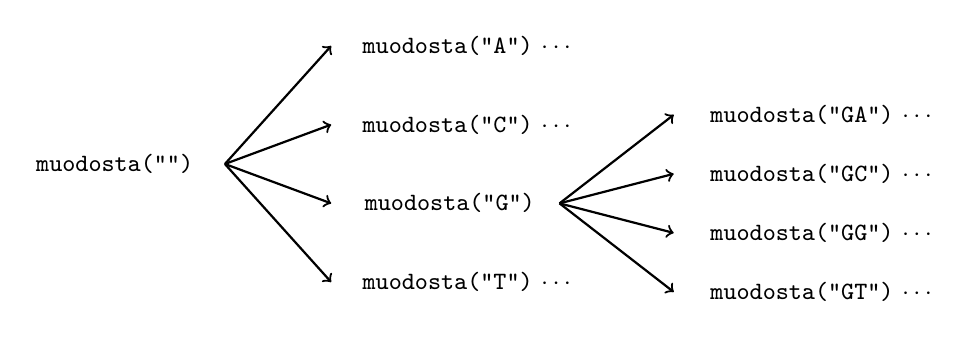
\begin{tikzpicture}[scale=0.5]
\small
\node at (-0.5,0) {\texttt{muodosta("\hspace{0pt}")}};
\node at (8.5,3) {\texttt{muodosta("A")} $\cdots$};
\node at (8.5,1) {\texttt{muodosta("C")} $\cdots$};
\node at (8.5,-1) {\texttt{muodosta("G")} $\phantom{\cdots}$};
\node at (8.5,-3) {\texttt{muodosta("T")} $\cdots$};
\draw[thick,->] (2.3,0) -- (5,3);
\draw[thick,->] (2.3,0) -- (5,1);
\draw[thick,->] (2.3,0) -- (5,-1);
\draw[thick,->] (2.3,0) -- (5,-3);
\node at (17.5,1.25) {\texttt{muodosta("GA")} $\cdots$};
\node at (17.5,-0.25) {\texttt{muodosta("GC")} $\cdots$};
\node at (17.5,-1.75) {\texttt{muodosta("GG")} $\cdots$};
\node at (17.5,-3.25) {\texttt{muodosta("GT")} $\cdots$};
\draw[thick,->] (10.8,-1) -- (13.7,1.25);
\draw[thick,->] (10.8,-1) -- (13.7,-0.25);
\draw[thick,->] (10.8,-1) -- (13.7,-1.75);
\draw[thick,->] (10.8,-1) -- (13.7,-3.25);
\end{tikzpicture}
\caption{DNA-ketjujen muodostaminen rekursiivisesti.}
\label{fig:ketjut}
\end{figure}

Kuva \ref{fig:ketjut} havainnollistaa,
kuinka funktio lähtee muodostamaan ketjuja tyhjästä ketjusta alkaen.
Ensin funktio haarautuu neljään osaan sen mukaan,
onko ketjun ensimmäinen merkki A, C, G vai T.
Tämän jälkeen haarautuminen jatkuu vastaavasti
jokaisessa kutsussa:
esimerkiksi jos ketju alkaa merkillä G,
funktio haarautuu tapauksiin GA, GC, GG ja GT, jne.

\subsection{Osajoukot ja permutaatiot}

Yksi tavallinen rekursion käyttötarkoitus on,
että haluamme käydä läpi kaikki annetun joukon \emph{osajoukot}
eli kaikki tavat valita jokin kokoelma joukon alkioita.
Esimerkiksi joukon $\{1,2,3\}$ osajoukot ovat
$\emptyset$ (tyhjä joukko), $\{1\}$, $\{2\}$, $\{3\}$,
$\{1,2\}$, $\{1,3\}$, $\{2,3\}$ ja $\{1,2,3\}$.
Kun joukossa on $n$ alkioita, osa\-joukkoja on yhteensä $2^n$.

Seuraava rekursiivinen funktio muodostaa joukon
$\{1,2,\dots,n\}$ osajoukot.
Haku lähtee käyntiin, kun kutsumme funktiota
parametrilla $1$.

\begin{code}
function muodosta(x)
    if x == n+1
        // käsittele osajoukko
    else
        valittu[x] = true
        muodosta(x+1)
        valittu[x] = false
        muodosta(x+1)
\end{code}

Ideana on, että parametri $x$ tarkoittaa, minkä alkion
''kohtalon'' ratkaisemme seuraavaksi: joko lisäämme alkion
osajoukkoon tai jätämme sen osa\-joukon ulkopuolelle.
Ensin päätämme, kuuluuko alkio $1$ osajoukkoon vai ei,
sitten toimimme vastaavasti alkion $2$ kohdalla, jne.,
kunnes olemme käsitelleet kaikki $n$ alkiota.
Jokaisen alkion kohdalla merkitsemme päätöksemme taulukkoon
\texttt{valittu} ja jatkamme osajoukon muodostamista rekursiivisesti.
Rekursio päät\-tyy, kun $x=n+1$ eli olemme tehneet valinnan
jokaiselle alkiolle ja olemme saaneet jonkin osajoukon muodostettua.
Tällöin voimme käsitellä muodostetun osajoukon haluamallamme tavalla.
Esimerkiksi voisimme tulostaa osajoukkoon kuuluvat alkiot seuraavasti:

\begin{code}
for i = 1 to n
    if valittu[i]
        print(i)
\end{code}

Tarkastellaan sitten toista tilannetta, jossa haluammekin
muodostaa joukon \emph{permutaatiot}
eli kaikki mahdolliset joukon alkioiden järjestykset.
Esimerkiksi joukon $\{1,2,3\}$ permutaatiot ovat
$(1,2,3)$, $(1,3,2)$, $(2,1,3)$, $(2,3,1)$, $(3,1,2)$ ja $(3,2,1)$.
Kun joukossa on $n$ alkiota, voimme muodostaa siitä yhteensä $n!$ permutaatiota.

Myös permutaatioiden läpikäynti onnistuu kätevästi rekursiolla.
Seuraava rekursiivinen funktio muodostaa joukon $\{1,2,\dots,n\}$ permutaatiot,
kun kutsumme sitä parametrilla $1$.

\begin{code}
muodosta(k)
    if k == n+1
        // käsittele permutaatio
    else
        for i = 1 to n
            if not valittu[i]
                valittu[i] = true
                permutaatio[k] = i
                muodosta(k+1)
                valittu[i] = false
\end{code}

Tässä parametri $k$ tarkoittaa, mihin permutaation kohtaan
valitsemme seuraavaksi alkion.
Aluksi valitsemme alkion kohtaan $1$, sitten
valitsemme alkion kohtaan $2$, jne., kohtaan $n$ asti.
Jokaisessa kohdassa käymme läpi silmukalla kaikki mahdolliset alkiot.
Taulukko \texttt{valittu} kertoo, mitkä alkiot olemme jo valinneet
permutaatioon.
Jos alkio $i$ ei ole vielä mukana permutaatiossa, haaraudumme tapaukseen,
jossa valitsemme sen kohtaan $k$ ja merkitsemme tämän tiedon
taulukkoon \texttt{permutaatio}.
Lopulta kun $k=n+1$, olemme saaneet muodostettua jonkin permutaation
ja rekursiivinen haarautuminen päättyy.
Tällöin voimme käsitellä permutaation haluamallamme tavalla,
esimerkiksi tulostaa alkioiden järjestyksen seuraavasti:

\begin{code}
for i = 1 to n
    print(permutaatio[i])
\end{code}

\subsection{Peruuttava haku}

\emph{Peruuttava haku} on yleinen rekursiivinen menetelmä,
jota käyttäen voimme muodostaa järjestelmällisesti
kaikki ratkaisut annettuun ongelmaan.
Ideana on aloittaa tyhjästä ratkaisusta ja käydä
joka askeleella läpi rekursiivisesti kaikki mahdolliset tavat,
kuinka voimme laajentaa ratkaisua.

Peruuttava haku on raa'an voiman menetelmä,
ja voimme käyttää sitä vain silloin,
kun ratkaisujen määrä on niin pieni,
että ehdimme käydä läpi kaikki ratkaisut.
Kuitenkin jos voimme käyttää peruuttavaa hakua,
se on mainio tekniikka,
koska voimme olla varmoja, että oikein toteutettu
peruuttava haku löytää kaikki ratkaisut.

\begin{figure}
\center
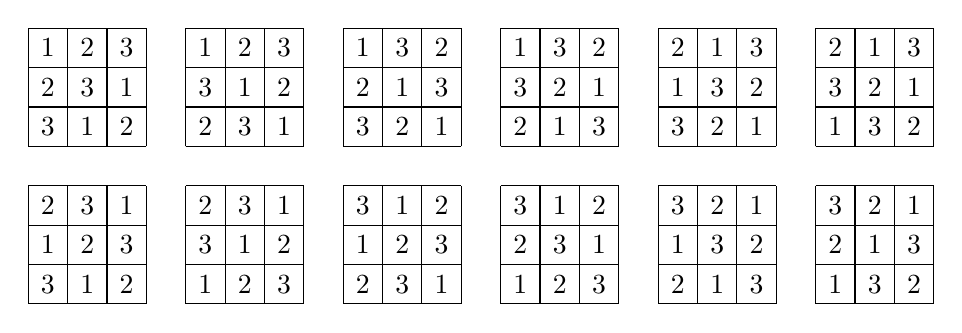
\begin{tikzpicture}[scale=0.5]
\newcommand\nelio[9]{
\draw (0,0) grid (3,3);
\foreach \x/\y/\v in {0/0/#1,1/0/#2,2/0/#3,0/1/#4,1/1/#5,2/1/#6,0/2/#7,1/2/#8,2/2/#9} \node at (0.5+\x,2.5-\y) {\v};
}
\begin{scope}
\nelio{1}{2}{3}{2}{3}{1}{3}{1}{2}
\end{scope}
\begin{scope}[xshift=4cm]
\nelio{1}{2}{3}{3}{1}{2}{2}{3}{1}
\end{scope}
\begin{scope}[xshift=8cm]
\nelio{1}{3}{2}{2}{1}{3}{3}{2}{1}
\end{scope}
\begin{scope}[xshift=12cm]
\nelio{1}{3}{2}{3}{2}{1}{2}{1}{3}
\end{scope}
\begin{scope}[xshift=16cm]
\nelio{2}{1}{3}{1}{3}{2}{3}{2}{1}
\end{scope}
\begin{scope}[xshift=20cm]
\nelio{2}{1}{3}{3}{2}{1}{1}{3}{2}
\end{scope}
\begin{scope}[yshift=-4cm]
\nelio{2}{3}{1}{1}{2}{3}{3}{1}{2}
\end{scope}
\begin{scope}[yshift=-4cm,xshift=4cm]
\nelio{2}{3}{1}{3}{1}{2}{1}{2}{3}
\end{scope}
\begin{scope}[yshift=-4cm,xshift=8cm]
\nelio{3}{1}{2}{1}{2}{3}{2}{3}{1}
\end{scope}
\begin{scope}[yshift=-4cm,xshift=12cm]
\nelio{3}{1}{2}{2}{3}{1}{1}{2}{3}
\end{scope}
\begin{scope}[yshift=-4cm,xshift=16cm]
\nelio{3}{2}{1}{1}{3}{2}{2}{1}{3}
\end{scope}
\begin{scope}[yshift=-4cm,xshift=20cm]
\nelio{3}{2}{1}{2}{1}{3}{1}{3}{2}
\end{scope}
\end{tikzpicture}
\caption{Kaikki 12 latinalaista neliötä kokoa $3 \times 3$.}
\label{fig:latnel}
\end{figure}

Tarkastellaan esimerkkinä tehtävää, jossa haluamme käydä läpi
kaikki kokoa $n \times n$ olevat \emph{latinalaiset neliöt}
eli ruudukot, joissa kullakin vaaka- ja pystyrivillä
esiintyy tarkalleen kerran jokainen luku $1,2,\dots,n$.
Kyseessä on siis yksinkertaistus tutusta sudoku-tehtävästä.
Esimerkiksi kuva \ref{fig:latnel} näyttää kaikki 12 latinalaista neliötä kokoa $3 \times 3$.

Toteutamme peruuttavan haun niin, että valitsemme joka askeleella
ruudukon kohtaan $(y,x)$ tulevan luvun.
Numeroimme ruudukon vaaka- ja pystyrivit kokonaisluvuin $1,2,\dots,n$.
Aloitamme haun ruudukon vasemmasta yläkul\-masta ja etenemme
rivi kerrallaan alaspäin.
Seuraava rekursiivinen algoritmi toteuttaa haun,
kun sitä kutsutaan parametreilla $(1,1)$:

\begin{code}
muodosta(y,x)
    if y == n+1
        // käsittele ratkaisu
    else if x == n+1
        muodosta(y+1,1)
    else
        for i = 1 to n
            if not vaaka[y][i] and not pysty[x][i]
                vaaka[y][i] = pysty[x][i] = true
                nelio[y][x] = i
                muodosta(y,x+1)
                vaaka[y][i] = pysty[x][i] = false
\end{code}

Algoritmin alussa on kaksi erikoistapausta:
jos $y=n+1$, olemme saaneet muodostettua
yhden latinalaisen neliön.
Jos taas $x=n+1$, olemme saaneet jonkin vaakarivin
valmiiksi ja alamme muodostaa seuraavaa vaakariviä.
Muuten kyseessä on perustapaus, jossa haluamme
valita kohtaan $(y,x)$ tulevan luvun.
Käymme läpi kaikki mahdolliset tavat for-silmukalla,
jossa $i$ on valittava luku.
Koska jokainen luku saa esiintyä vain kerran kullakin
vaaka- ja pystyrivillä, käytämme kahta aputaulukkoa:
$\texttt{vaaka}[y][i]$ kertoo, onko vaakarivillä $y$
jo lukua $i$, ja vastaavasti $\texttt{pysty}[x][i]$ kertoo,
onko pystyrivillä $x$ jo lukua $i$.
Jos voimme sijoittaa luvun $i$ kohtaan $(y,x)$,
merkitsemme tämän taulukkoon $\texttt{nelio}[y][x]$
ja lisäksi päivitämme taulukoita $\texttt{vaaka}$ ja $\texttt{pysty}$.
Sitten jatkamme hakua rekursiivisesti seuraavaan
oikealla olevaan ruutuun.

\begin{table}
\center
\begin{tabular}{rr}
ruudukon koko $n$ & neliöiden määrä \\
\hline
1 & 1 \\
2 & 2 \\
3 & 12 \\
4 & 576 \\
5 & 161280 \\
6 & 812851200 \\
\end{tabular}
\caption{Latinalaisten neliöiden määrät, kun $n=1,2,\dots,6$.}
\label{tab:latnel}
\end{table}

Kun olemme saaneet muodostettua latinalaisen neliön, voimme käsitellä
sen haluamallamme tavalla, kuten tulostaa neliön sisältö
taulukon \texttt{nelio} perusteella
tai vain laskea, montako neliötä on olemassa.
Taulukko \ref{tab:latnel} listaa latinalaisten neliöiden
määrät arvoilla $n=1,2,\dots,6$, jotka pystymme laskemaan
nopeasti tässä esitetyn algoritmin avulla.
Suuremmilla $n$:n arvoilla haku alkaa kestää liian kauan
ja meidän tulisi keksiä keino tehostaa hakua,
jos haluaisimme laskea määriä suuremmissa tapauksissa.

\section{Matemaattinen tausta}

Tietorakenteiden ja algoritmien teoria perustuu matematiikkaan,
ja käym\-me kirjassa pikkuhiljaa läpi tarvittavia tietoja.
Seuraavassa on joitakin merkintöjä ja käsitteitä, joista on hyötyä
useassa kirjan kohdassa.

\subsection{Summakaavat}

Voimme laskea lukujen $1,2,\dots,n$ summan kaavalla
\[1+2+\dots+n = \frac{n(n+1)}{2}.\]
Esimerkiksi
\[1+2+3+4+5 = \frac{5 \cdot 6}{2}=15.\]
Kaavan voi ymmärtää niin, että laskemme yhteen $n$ lukua,
joiden suuruus on \emph{keskimäärin} $(n+1)/2$.

Toinen hyödyllinen kaava on
\[2^0+2^1+\dots+2^n = 2^{n+1}-1.\]
Esimerkiksi
\[1+2+4+8+16=32-1.\]
Tässä voimme ajatella, että aloitamme luvusta $2^n$
ja lisäämme siihen aina puolet pienemmän luvun lukuun $1$ asti.
Tämän seurauksena pääsemme yhtä vaille lukuun $2^{n+1}$ asti.

Esitämme joskus summia merkinnän $\sum$ avulla.
Siinä on ideana antaa muuttujan ala- ja yläraja sekä
joka askeleella summaan lisättävä arvo.
Esimerkiksi voimme merkitä
\[1^2 + 2^2 + \dots + n^2 = \sum_{i=1}^n i^2.\]

Tämä merkintä on itse asiassa hyvin lähellä ohjelmoinnin
for-silmukkaa, koska seuraava koodi ajaa saman asian:

\begin{code}
summa = 0
for i = 1 to n
    summa += i*i
\end{code}

\subsection{Logaritmit}

Logaritmin määritelmän mukaan $\log_b n =x$
tarkalleen silloin kun $b^x=n$.
Esimerkiksi $\log_2 32=5$, koska $2^5=32$.

Algoritmiikassa logaritmin kantaluku $b$ on usein 2,
ja voimme ajatella, että logaritmi kertoo, montako kertaa
meidän täytyy \emph{puolittaa} luku $n$, ennen kuin pääsemme lukuun 1.
Esimerkiksi $\log_2 32 =5$, koska tarvitsemme 5 puolitusta:
\[32 \rightarrow 16 \rightarrow 8 \rightarrow 4 \rightarrow 2 \rightarrow 1\]
Tässä kirjassa oletamme, että logaritmin kantaluku on 2,
jos ei ole toisin mainittu,
eli voimme kirjoittaa lyhyesti $\log 32 = 5$.

Logaritmeille pätee kaavat
\[\log_b(x \cdot y) = \log_b(x)+\log_b(y)\]
ja
\[\log_b(x / y) = \log_b(x)-\log_b(y).\]
Ylemmästä kaavasta seuraa myös
\[\log_b(x^k) = k \log_b(x).\]
Lisäksi voimme vaihtaa logaritmin kantalukua kaavalla
\[\log_u(x) = \frac{\log_b(x)}{\log_b(u)}.\]
\chapter{Tehokkuus}

Algoritmien suunnittelussa tavoitteemme on saada aikaan
algoritmeja, jotka toimivat \emph{tehokkaasti}.
Haluamme luoda algoritmeja, joiden avulla voimme
käsitellä myös suuria aineistoja ilman, että joudumme
odottamaan kauan aikaa.
Ajattelemmekin, että algoritmi on \emph{hyvä},
jos se kykenee antamaan meille nopean vastauksen myös silloin,
kun annamme sille paljon tietoa.

Tässä luvussa tutustumme työkaluihin, joiden avulla
voimme arvioida algoritmien tehokkuutta.
Keskeinen käsite on \emph{aikavaativuus}, joka antaa
tiiviissä muodossa kuvauksen algoritmin ajankäytöstä.
Aikavaativuuden avulla voimme muodostaa arvion
algoritmin tehokkuudesta sen rakenteen perusteella,
eikä meidän tarvitse toteuttaa ja testata algoritmia
vain saadaksemme tietää, miten nopea se on.

\section{Aikavaativuus}

\index{aikavaativuus}

Algoritmin tehokkuus riippuu siitä, montako askelta se suorittaa.
Tavoitteemme on nyt arvioida algoritmin askelten määrää
suhteessa syötteen kokoon $n$.
Esimerkiksi jos syötteenä on taulukko,
$n$ on taulukon koko,
ja jos syötteenä on merkkijono,
$n$ on merkkijonon pituus.

Tarkastellaan esimerkkinä seuraavaa algoritmia,
joka laskee, montako kertaa alkio $x$ esiintyy
$n$ lukua sisältävässä taulukossa.

\begin{code}[numbers=left]
laskuri = 0
for i = 0 to n-1
    if luvut[i] == x
        laskuri++
\end{code}

Voimme arvioida algoritmin tehokkuutta tutkimalla
jokaisesta rivistä, montako kertaa algoritmi suorittaa sen.
Rivi 1 suoritetaan vain kerran algoritmin alussa.
Tämän jälkeen alkaa silmukka, jossa
rivit 2 ja 3 suoritetaan molemmat $n$ kertaa
ja rivi 4 puolestaan suoritetaan $0 \dots n$
kertaa riippuen siitä, kuinka usein
luku $x$ esiintyy taulukossa.
Algoritmi suorittaa siis vähintään $2n+1$ ja enintään $3n+1$
askelta.

\index{$O$-merkintä}

Näin tarkka analyysi ei ole kuitenkaan yleensä tarpeen,
vaan meille riittää määrittää karkea \emph{yläraja} ajankäytölle.
Sanomme, että algoritmi toimii ajassa $O(f(n))$ eli sen
\emph{aikavaativuus} (\emph{time complexity}) on $O(f(n))$, jos se suorittaa
enintään $c f(n)$ askelta aina silloin kun $n \ge n_0$,
missä $c$ ja $n_0$ ovat vakioita.
Esimerkiksi yllä oleva algoritmi toimii ajassa $O(n)$,
koska se suorittaa selkeästi enintään $4n$ askelta
kaikilla $n$:n arvoilla.

\subsection{Laskusääntöjä}

Aikavaativuuden mukavana puolena on, että voimme yleensä
päätellä aikavaativuuden helposti algoritmin
rakenteesta. Tutustumme seuraavaksi laskusääntöihin,
joiden avulla tämä on mahdollista.

\subsubsection{Yksittäiset komennot}

Jos koodissa ei ole silmukoita vaan vain
yksittäisiä komentoja, sen aikavaativuus on $O(1)$.
Näin on esimerkiksi seuraavassa koodissa:

\begin{code}
c = a+b
if c >= 0
    print(c)
\end{code}

\subsubsection{Silmukat}

Merkitsemme \texttt{...} koodia,
jonka aikavaativuus on $O(1)$.
Jos koodissa on yksi silmukka,
joka suorittaa $n$ askelta,
sen aikavaativuus on $O(n)$:

\begin{code}
for i = 1 to n
    ...
\end{code}

Jos tällaisia silmukoita on kaksi sisäkkäin,
aikavaativuus on $O(n^2)$:

\begin{code}
for i = 1 to n
    for j = 1 to n
        ...
\end{code}

Yleisemmin jos koodissa on vastaavalla tavalla
$k$ sisäkkäistä silmukkaa, sen aikavaativuus on $O(n^k)$.

\index{vakiokerroin}

Huomaa, että vakiokertoimet ja matalammat termit eivät vaikuta aikavaativuuteen.
Esimerkiksi seuraavissa koodeissa silmukoissa on $2n$ ja $n-1$ askelta,
mutta kummankin koodin aikavaativuus on $O(n)$.

\begin{code}
for i = 1 to 2*n
    ...
\end{code}

\begin{code}
for i = 1 to n-1
    ...
\end{code}

\subsubsection{Peräkkäiset osuudet}

Jos koodissa on peräkkäisiä osuuksia, sen aikavaativuus on suurin
yksittäisen osuuden aikavaativuus. Esimerkiksi seuraavan koodin aikavaativuus on $O(n^2)$,
koska sen osuuksien aikavaativuudet ovat $O(n)$, $O(n^2)$ ja $O(n)$.

\begin{code}
for i = 1 to n
    ...
for i = 1 to n
    for j = 1 to n
        ...
for i = 1 to n
    ...
\end{code}

\subsubsection{Monta muuttujaa}

Joskus aikavaativuus riippuu useammasta tekijästä,
jolloin kaavassa on monta muuttujaa.
Esimerkiksi seuraavan koodin aikavaativuus on $O(nm)$:

\begin{code}
for i = 1 to n
    for j = 1 to m
        ...
\end{code}

\subsubsection{Rekursiiviset algoritmit}

Rekursiivisessa algoritmissa laskemme,
montako rekursiivista kutsua teh\-dään ja kauanko
yksittäinen kutsu vie aikaa.
Tarkastellaan esimerkkinä seuraavaa
aliohjelmaa, jota kutsutaan parametrilla $n$:

\begin{code}
procedure f(n)
    if n == 1
        return
    f(n-1)
\end{code}

Aliohjelmaa kutsutaan yhteensä $n$ kertaa ja jokainen kutsu vie aikaa $O(1)$.
Saamme selville aliohjelman aikavaativuuden kertomalla nämä arvot keskenään,
joten aliohjelma vie aikaa $O(n)$.

Tarkastellaan sitten seuraavaa aliohjelmaa:

\begin{code}
procedure g(n)
    if n == 1
        return
    g(n-1)
    g(n-1)
\end{code}

Tässä tapauksessa jokainen aliohjelman kutsu tuottaa kaksi uutta kutsua,
joten aliohjelmaa kutsutaan kaikkiaan
\[1+2+4+\dots+2^{n-1}=2^n-1\]
kertaa. Jokainen kutsu vie aikaa $O(1)$,
joten aikavaativuus on $O(2^n)$.

\subsection{Yleisiä aikavaativuuksia}

Tietyt aikavaativuudet esiintyvät usein algoritmeissa.
Käymme seuraavaksi läpi joukon tällaisia aikavaativuuksia.

\index{vakioaikainen algoritmi}

\subsubsection{$O(1)$ (vakioaikainen)}

\emph{Vakioaikainen} (\emph{constant time}) algoritmi suorittaa kiinteän määrän komentoja,
eikä syötteen suuruus vaikuta algoritmin nopeuteen.
Esimerkiksi seuraava algoritmi laskee summan $1+2+\dots+n$
vakioajassa kaavalla $n(n+1)/2$:

\begin{code}
summa = n*(n+1)/2
\end{code}

\index{logaritminen algoritmi}

\subsubsection{$O(\log n)$ (logaritminen)}

\emph{Logaritminen} (\emph{logarithmic}) algoritmi puolittaa usein syötteen koon
joka askeleella.
Esimerkiksi seuraavan algoritmin aikavaativuus on $O(\log n)$:

\begin{code}
laskuri = 0
while n >= 1
    laskuri++
    n /= 2
\end{code}

Tärkeä seikka logaritmeihin liittyen on, että
$\log n$ on \emph{pieni} luku, kun $n$ on mikä tahansa 
tyypillinen algoritmeissa esiintyvä luku.
Esimerkiksi $\log 10^6 \approx 20$ ja $\log 10^9 \approx 30$,
kun logaritmin kantaluku on 2.
Niinpä jos algoritmi tekee jotain logaritmisessa ajassa,
siinä ei kulu kauan aikaa.

\index{lineaarinen algoritmi}

\subsubsection{$O(n)$ (lineaarinen)}

\emph{Lineaarinen} (\emph{linear}) algoritmi voi käydä läpi syötteen kiinteän määrän kertoja.
Esimerkiksi seuraava $O(n)$-algoritmi laskee taulukon lukujen summan:

\begin{code}
summa = 0
for i = 0 to n-1
    summa += taulu[i]
\end{code}

Kun algoritmin syötteenä on aineisto, jossa on $n$ alkiota,
lineaarinen aikavaativuus on yleensä paras mahdollinen,
minkä voimme saavuttaa.
Tämä johtuu siitä, että algoritmin täytyy käydä syöte
ainakin kerran läpi, ennen kuin se voi ilmoittaa vastauksen.

\subsubsection{$O(n \log n)$ (järjestäminen)}

Aikavaativuus $O(n \log n)$ viittaa usein siihen,
että algoritmin osana on \emph{järjes\-tämistä},
koska tehokkaat järjestämisalgoritmit
toimivat ajassa $O(n \log n)$.
Esimerkiksi seuraava $O(n \log n)$-aikainen
algoritmi tarkastaa, onko taulukossa kahta samaa alkiota:

\begin{code}
sort(taulu) // järjestäminen
samat = false
for i = 1 to n-1
    if taulu[i] == taulu[i-1]
        samat = true
\end{code}

Algoritmi järjestää ensin taulukon, minkä jälkeen yhtä
suuret alkiot ovat vierekkäin ja ne on helppoa löytää.
Järjestäminen vie aikaa $O(n \log n)$
ja silmukka vie aikaa $O(n)$, joten algoritmi vie
yhteensä aikaa $O(n \log n)$.

Tutustumme tarkemmin järjestämiseen ja sitä käyttäviin
algoritmeihin seuraavassa luvussa 3.

\index{neliöllinen algoritmi}

\subsubsection{$O(n^2)$ (neliöllinen)}

\emph{Neliöllinen} (\emph{quadratic}) algoritmi voi käydä läpi kaikki tavat valita
kaksi alkiota syöt\-teestä.
Esimerkiksi seuraava $O(n^2)$-algoritmi tutkii, onko taulukossa
kahta lukua, joiden summa on $x$.

\begin{code}
ok = false
for i = 0 to n-1
    for j = i+1 to n-1
        if taulu[i]+taulu[j] == x
            ok = true
\end{code}

\index{kuutiollinen algoritmi}

\subsubsection{$O(n^3)$ (kuutiollinen)}

\emph{Kuutiollinen} (\emph{cubic}) algoritmi voi käydä läpi kaikki tavat valita
kolme alkiota syöt\-teestä.
Esimerkiksi seuraava $O(n^3)$-algoritmi tutkii, onko taulukossa
kolmea lukua, joiden summa on $x$.

\begin{code}
ok = false
for i = 0 to n-1
    for j = i+1 to n-1
        for k = j+1 to n-1
            if taulu[i]+taulu[j]+taulu[k] == x
                ok = true
\end{code}

\subsubsection{$O(2^n)$ (osajoukot)}

Aikavaativuus $O(2^n)$ viittaa usein siihen,
että algoritmi käy läpi syötteen alkioiden osajoukot.

\subsubsection{$O(n!)$ (permutaatiot)}

Aikavaativuus $O(n!)$ viittaa usein siihen,
että algoritmi käy läpi syötteen alkioiden permutaatiot.

\subsection{Tehokkuuden arviointi}

Mitä hyötyä on määrittää algoritmin aikavaativuus?
Hyötynä on, että aikavaativuus antaa meille arvion siitä,
kuinka \emph{hyvä} algoritmi on eli miten suuria syötteitä
sillä voi käsitellä tehokkaasti.
Kun meille kertyy kokemusta algoritmien suunnittelusta,
meille alkaa muodostua selkeä kuva,
mitä eri aikavaativuudet tarkoittavat käytännössä.

Aikavaativuutta voi ajatella samalla tavalla kuin vaikkapa
hotellin tähti\-luokitusta: se kertoo tiiviissä muodossa,
mistä asiassa on kysymys, eikä mei\-dän tarvitse ottaa selvää yksityiskohdista.
Jos meille tarjotaan majoitusta neljän tähden hotellissa,
saamme heti jonkin käsityksen huoneen tasosta
tähtiluokituksen ansiosta,
vaikka emme saisi tarkkaa listausta huoneen varustelusta.
Vastaavasti jos kuulemme, että jonkin algoritmin aikavaativuus on $O(n \log n)$,
voimme heti arvioida karkeasti, miten suuria syötteitä voimme käsitellä,
vaikka emme tuntisi tarkemmin algoritmin toimintaa.

\begin{table}
\center
\begin{tabular}{rrr}
syötteen kokoluokka $n$ & tarvittava aikavaativuus \\
\hline
10 & $O(n!)$ \\
20 & $O(2^n)$ \\
500 & $O(n^3)$ \\
5000 & $O(n^2)$ \\
$10^6$ & $O(n)$ tai $O(n \log n)$ \\
suuri & $O(1)$ tai $O(\log n)$ \\
\end{tabular}
\caption{Kuinka suuren syötteen algoritmi voi käsitellä nopeasti?}
\label{tab:algteh}
\end{table}

Yksi kiinnostava näkökulma algoritmin tehokkuuteen on,
miten suuren syötteen algoritmi voi käsitellä \emph{nopeasti}
(alle sekunnissa).
Tämä on hyvä vaatimus, kun haluamme käyttää algoritmia
jossakin käytännön sovelluksessa.
Taulukossa \ref{tab:algteh} on joitakin hyödyllisiä arvioita,
kun Java-kielellä toteutettu
algoritmi suoritetaan nykyaikaisella tietokoneella.
Esimerkiksi jos meillä on $O(n^2)$-algoritmi, voimme käsitellä sillä
nopeasti syötteen, jossa on luokkaa 5000 alkiota.
Jos haluamme käsitellä tehokkaasti suurempia syötteitä,
meidän tulisi löytää $O(n)$- tai $O(n \log n)$-aikainen algoritmi.

Kannattaa silti pitää mielessä, että nämä luvut ovat vain arvioita ja algoritmin
todelliseen ajankäyttöön vaikuttavat monet asiat.
Saman algoritmin hyvä toteutus saattaa olla
kymmeniä kertoja nopeampi kuin huono toteutus,
ja suuri merkitys on myös ohjelmointikielellä,
jolla algoritmi on toteutettu.
Tässä kirjassa analysoimme algoritmeja sekä aikavaativuuksien
avulla että mittaamalla todellisia suoritusaikoja.

\subsection{Esimerkki: Merkkijonot}

Tehtävän ratkaisemiseen on usein monenlaisia algoritmeja.
Seuraavaksi ratkaisemme saman tehtävän kahdella algoritmilla,
joista ensimmäinen on suoraviivainen raa'an voiman
algoritmi, joka toimii ajassa $O(n^2)$.
Toinen algoritmi on puolestaan tehokas algoritmi,
joka vie aikaa vain $O(n)$.

Tehtävämme on seuraava: Annettuna on merkkijono,
jonka pituus on $n$ ja jokainen merkki on 0 tai 1.
Haluamme laskea, monellako tavalla voimme valita kaksi kohtaa
niin, että vasen merkki on 0 ja oikea merkki on 1.
Esimerkiksi merkkijonossa 01001 tapoja on neljä:
\underline{01}001, \underline{0}100\underline{1},
01\underline{0}0\underline{1} ja 010\underline{01}.

\subsubsection{$O(n^2)$-algoritmi}

Voimme ratkaista tehtävän raa'alla voimalla
käymällä läpi kaikki mahdolliset tavat valita vasen ja oikea kohta.
Tällöin voimme laskea yksi kerrallaan,
monessako tavassa vasen merkki on 0 ja oikea merkki on 1.
Seuraava koodi toteuttaa algoritmin:

\begin{code}
laskuri = 0
for i = 0 to n-1
    for j = i+1 to n-1
        if merkit[i] == 0 and merkit[j] == 1
            laskuri++
print(laskuri)
\end{code}

Algoritmin aikavaativuus on $O(n^2)$, koska siinä on kaksi
sisäkkäistä silmukkaa, jotka käyvät läpi syötteen.

\subsubsection{$O(n)$-algoritmi}

Kuinka voisimme ratkaista tehtävän tehokkaammin?
Meidän tulisi keksiä tapa, jolla saisimme
pois toisen silmukan koodista.

Tässä auttaa lähestyä ongelmaa hieman toisesta
näkökulmasta: kun olemme tietyssä kohdassa merkkijonoa,
monellako tavalla voimme muodostaa parin,
jonka oikea merkki on nykyisessä kohdassamme?
Jos olemme merkin 0 kohdalla, pareja ei ole yhtään,
mutta jos merkkinä on 1, voimme valita \emph{minkä tahansa}
vasemmalla puolella olevan merkin 0 pariin.

Tämän havainnon ansiosta meidän riittää käydä läpi
merkkijono kerran vasemmalta oikealle ja pitää kirjaa,
montako merkkiä 0 olemme nähneet.
Sitten jokaisen merkin 1 kohdalla kasvatamme
vastausta tämänhetkisellä merkkien 0 määrällä.
Seuraava koodi toteuttaa algoritmin:

\begin{code}
laskuri = 0
nollat = 0
for i = 0 to n-1
    if merkit[i] == 0
        nollat++
    else
        laskuri += nollat
print(laskuri)
\end{code}

Algoritmissa on vain yksi silmukka, joka käy syötteen läpi,
joten sen aikavaativuus on $O(n)$.

\subsubsection{Algoritmien vertailua}

Meillä on nyt siis kaksi algoritmia, joiden aikavaativuudet ovat
$O(n^2)$ ja $O(n)$, mutta mitä tämä tarkoittaa käytännössä?
Saamme tämän selville toteuttamalla algoritmit jollakin
oikealla ohjelmointikielellä
ja mittaamalla niiden suoritusaikoja erikokoisilla syötteillä.

Taulukko \ref{tab:algver} näyttää vertailun tulokset,
kun algoritmit on toteutettu Javalla ja syötteinä
on satunnaisia merkkijonoja.
Pienillä $n$:n arvoilla molemmat algoritmit toimivat
hyvin tehokkaasti, mutta suuremmilla syötteillä on
nähtävissä huomattavia eroja.
Raakaan voimaan perustuva $O(n^2)$-algoritmi
alkaa hidastua selvästi testistä $n=10^4$ alkaen,
ja testissä $n=10^6$ sillä kuluu jo lähes kolme minuuttia aikaa.
Tehokas $O(n)$-algoritmi taas selvittää suuretkin testit
salamannopeasti.

\begin{table}
\center
\begin{tabular}{rrr}
syötteen koko $n$ & $O(n^2)$-algoritmi & $O(n)$-algoritmi \\
\hline
$10$ & 0.00 s & 0.00 s\\
$10^2$ & 0.00 s & 0.00 s\\
$10^3$ & 0.00 s & 0.00 s\\
$10^4$ & 0.14 s & 0.00 s \\
$10^5$ & 1.66 s & 0.00 s \\
$10^6$ & 172.52 s & 0.01 s \\
\end{tabular}
\caption{Algoritmien suoritusaikojen vertailu.}
\label{tab:algver}
\end{table}

Tämän kurssin jatkuvana teemana on luoda algoritmeja,
jotka toimivat tehokkaasti myös silloin, kun niille annetaan suuria syötteitä.
Tämä tarkoittaa käytännössä sitä, että algoritmin aikavaativuuden tulisi
olla $O(n)$ tai $O(n \log n)$.
Jos algoritmin aikavaativuus on esimerkiksi $O(n^2)$,
se on auttamatta liian hidas suurien syötteiden käsittelyyn.

\section{Lisää algoritmien analysoinnista}

Aikavaativuuksissa esiintyvä $O$-merkintä on yksi monista merkinnöistä,
joiden avulla voimme arvioida funktioiden kasvunopeutta.
Tutustumme seuraavaksi tarkemmin näihin merkintöihin.

\subsection{Merkinnät $O$, $\Omega$ ja $\Theta$}

\index{$O$-merkintä}
\index{$\Omega$-merkintä}
\index{$\Theta$-merkintä}

Algoritmien analysoinnissa usein esiintyviä merkintöjä ovat:

\begin{itemize}
\item \emph{Yläraja}: Funktio $g(n)$ on luokkaa $O(f(n))$, jos on olemassa vakiot $c$ ja $n_0$
niin, että $g(n) \le c f(n)$ aina kun $n \ge n_0$.
\item \emph{Alaraja}: Funktio $g(n)$ on luokkaa $\Omega(f(n))$, jos on olemassa vakiot $c$ ja $n_0$
niin, että $g(n) \ge c f(n)$ aina kun $n \ge n_0$.
\item \emph{Tarkka arvio}: Funktio $g(n)$ on luokkaa $\Theta(f(n))$, jos se on sekä luokkaa $O(f(n))$
että luokkaa $\Omega(f(n))$.
\end{itemize}

Vakion $c$ tarkoituksena on, että saamme arvion kasvunopeuden suuruusluokalle välittämättä
vakiokertoimista. Vakion $n_0$ ansiosta meidän riittää tarkastella
kasvunopeutta suurilla $n$:n arvoilla.
Voimme myös kirjoittaa $g(n)=O(f(n))$, kun haluamme ilmaista,
että funktio $g(n)$ on luokkaa $O(f(n))$,
ja vastaavasti $\Omega$- ja $\Theta$-merkinnöissä.

Kun sanomme, että algoritmi toimii ajassa $O(f(n))$, tarkoitamme, että se suorittaa
\emph{pahimmassa tapauksessa} $O(f(n))$ askelta.
Tämä on yleensä hyvä tapa ilmoittaa algoritmin tehokkuus,
koska silloin annamme takuun siitä, että algoritmin ajankäytöllä on tietty yläraja,
vaikka syöte olisi valittu mahdollisimman ikävästi algoritmin kannalta.

Tarkastellaan esimerkkinä seuraavaa algoritmia, joka laskee
taulukon lukujen summan:

\begin{code}
summa = 0
for i = 0 to n-1
    summa += taulu[i]
\end{code}

Tämä algoritmi toimii samalla tavalla riippumatta taulukon sisällöstä,
koska se käy aina läpi koko taulukon.
Niinpä yläraja ajankäytölle on $O(n)$ ja alaraja ajankäytölle on samoin $\Omega(n)$,
joten voimme sanoa, että algoritmi vie aikaa $\Theta(n)$ kaikissa tapauksissa.

Tarkastellaan sitten seuraavaa algoritmia, joka selvittää,
onko taulukossa lukua $x$:

\begin{code}
ok = false
for i = 0 to n-1
    if taulu[i] == x
        ok = true
        break
\end{code}

Tässä algoritmin pahin ja paras tapaus eroavat.
Ajankäytön yläraja on $O(n)$, koska algoritmi joutuu käymään
läpi kaikki taulukon alkiot silloin, kun luku $x$
ei esiinny taulukossa.
Toisaalta ajankäytön alaraja on $\Omega(1)$,
koska jos luku $x$ on taulukon ensimmäinen alkio,
algoritmi pysähtyy heti taulukon alussa.
Voimme myös sanoa, että algoritmi suorittaa pahimmassa
tapauksessa $\Theta(n)$ askelta ja parhaassa tapauksessa
$\Theta(1)$ askelta.

Huomaa, että $O$-merkinnän antama yläraja voi olla
\emph{mikä tahansa} yläraja, ei välttämättä tarkka yläraja.
On siis oikein sanoa esimerkiksi, että äskeinen
algoritmi vie aikaa $O(n^2)$, vaikka on olemassa parempi yläraja $O(n)$.
Miksi sitten käytämme $O$-merkintää, vaikka voisimme usein myös ilmaista tarkan
ajankäytön $\Theta$-merkinnällä?
Tämä on vakiintunut ja käytännössä toimiva tapa.
Olisi hyvin harhaanjohtavaa antaa algoritmille yläraja $O(n^2)$,
jos näemme suoraan, että aikaa kuluu vain $O(n)$.

Asiaa voi ajatella niin, että $O$-merkintää käytetään algoritmin
\emph{markkinoinnissa}. Jos annamme liian suuren ylärajan, algoritmista
tulee väärä käsitys yleisölle.
Vertauksena jos myymme urheiluautoa, jonka huippunopeus on 250 km/h,
on sinänsä paikkansa pitävä väite, että autolla pystyy ajamaan 100 km/h.
Meidän ei kuitenkaan kannata antaa tällaista vähättelevää tietoa,
vaan kertoa, että autolla pystyy ajamaan 250 km/h.

\subsection{Tilavaativuus}

\index{tilavaativuus}

Merkintöjä $O$, $\Omega$ ja $\Theta$ voi käyttää
kaikenlaisissa yhteyksissä, ei vain algoritmin ajankäytön arvioinnissa.
Esimerkiksi voimme sanoa, että algoritmi suorittaa silmukkaa $O(\log n)$ kierrosta
tai että taulukossa on $O(n^2)$ lukua.

Aikavaativuuden lisäksi kiinnostava tieto algoritmista voi olla sen
\emph{tilavaativuus} (\emph{space complexity}). Tämä kuvaa sitä, miten paljon algoritmi
käyttää muistia syötteen \emph{lisäksi}.
Jos tilavaativuus on $O(1)$, algoritmi tarvitsee muistia
vain yksittäisille muuttujille.
Jos tilavaativuus on $O(n)$, algoritmi voi varata esimerkiksi aputaulukon,
jonka koko vastaa syötteen kokoa.

Tarkastellaan esimerkkinä tehtävää, jossa taulukossa on
luvut $1,2,\dots,n$ yhtä lukuun ottamatta,
ja tehtävämme on selvittää puuttuva luku.
Yksi tapa ratkaista tehtävä $O(n)$-ajassa on luoda aputaulukko,
joka pitää kirjaa mukana olevista luvuista.
Tällaisen ratkaisun tilavaativuus on $O(n)$,
koska aputaulukko vie $O(n)$ muistia.

\begin{code}
for i = 0 to n-2
    mukana[taulu[i]] = true
for i = 1 to n
    if not mukana[i]
        puuttuva = i
\end{code}

Tehtävään on kuitenkin olemassa myös toinen algoritmi,
jossa aikavaativuus on edelleen $O(n)$ mutta tilavaativuus on vain $O(1)$.
Tällainen algoritmi laskee ensin lukujen $1,2,\dots,n$ summan
ja vähentää sitten taulukossa esiintyvät luvut siitä.
Jäljelle jäävä luku on puuttuva luku.

\begin{code}
summa = 0
for i = 1 to n
    summa += i
for i = 0 to n-2
    summa -= taulu[i]
puuttuva = summa
\end{code}

Käytännössä tilavaativuus on yleensä sivuroolissa algoritmeissa,
koska jos algoritmi vie vain vähän aikaa, se ei \emph{ehdi} käyttää kovin paljon muistia.
Erityisesti tilavaativuus ei voi olla suurempi kuin aikavaativuus.
Niinpä meidän riittää tavallisesti keskittyä suunnittelemaan algoritmeja,
jotka toimivat nopeasti, ja vertailla algoritmien aikavaativuuksia.

\subsection{Rajojen todistaminen}

Jos haluamme todistaa täsmällisesti, että jokin raja pätee,
meidän täytyy löytää vakiot $c$ ja $n_0$, jotka osoittavat asian.
Jos taas haluamme todistaa, että raja ei päde,
meidän täytyy näyttää, että mikään vakioiden $c$ ja $n_0$ valinta ei ole kelvollinen.

Jos haluamme todistaa rajan pätemisen,
tämä onnistuu yleensä helposti valitsemalla vakio $c$
tarpeeksi suureksi ja arvioimalla summan osia ylöspäin tarvittaessa.
Esimerkiksi jos haluamme todistaa, että $3n+5 = O(n)$, meidän tulee löytää
vakiot $c$ ja $n_0$, joille pätee, että $3n+5 \le cn$ aina kun $n \ge n_0$.
Tässä tapauksessa voimme valita esimerkiksi $c=8$ ja $n_0=1$,
jolloin voimme arvioida $3n+5 \le 3n+5n=8n$, kun $n \ge 1$.

Jos haluamme todistaa, että raja ei päde, tilanne on hankalampi,
koska meidän täytyy näyttää, että ei ole olemassa \emph{mitään} kelvollista
tapaa valita vakioita $c$ ja $n_0$.
Tässä auttaa tyypillisesti vastaoletuksen tekeminen: oletamme,
että raja pätee ja voimme valita vakiot,
ja näytämme sitten, että tämä oletus johtaa ristiriitaan.

Todistetaan esimerkkinä, että $n^2 \neq O(n)$.
Jos pätisi $n^2=O(n)$, niin olisi olemassa vakiot $c$ ja $n_0$,
joille $n^2 \le cn$ aina kun $n \ge n_0$.
Voimme kuitenkin osoittaa, että tämä aiheuttaa ristiriidan.
Jos $n^2 \le cn$, niin voimme jakaa epäyhtälön molemmat puolet $n$:llä
ja saamme $n \le c$.
Tämä tarkoittaa, että $n$ on aina enintään yhtä suuri kuin vakio $c$.
Tämä ei ole kuitenkaan mahdollista, koska $n$ voi olla miten
suuri tahansa, joten ei voi päteä $n^2 = O(n)$.

Määritelmistä lähtevä todistaminen on sinänsä mukavaa ajanvietettä,
mutta sille on äärimmäisen harvoin tarvetta käytännössä,
kun haluamme tutkia algoritmien tehokkuutta.
Voimme koko kurssin ajan huoletta päätellä algoritmin aikavaativuuden
katsomalla, mikä sen rakenne on, kuten olemme tehneet tämän luvun alkuosassa.

\chapter{Järjestäminen}

Järjestäminen on keskeinen algoritmiikan ongelma,
jolle on käyttöä sekä itsenäisenä algoritmina että
laajemman algoritmin osana.
Voimme ratkaista monia ongelmia järjestämällä
ensin aineiston, minkä jälkeen voimme hyö\-dyntää
järjestystä tavalla tai toisella.

Yksinkertaiset algoritmit järjestämiseen toimivat
ajassa $O(n^2)$, ja ne perustuvat kahteen sisäkkäiseen
silmukkaan.
Voimme kuitenkin järjestää taulukon myös tehokkaammin
ajassa $O(n \log n)$, mikä mahdollistaa järjestämisen
käyttämisen tehokkaiden algoritmien suunnittelussa.

Tässä luvussa tutustumme ensin järjestämisen teoriaan
ja erilaisiin järjes\-tämisalgoritmeihin.
Sitten luomme katsauksen siihen, kuinka voimme
käyttää järjestämistä Java-ohjelmoinnissa.
Lopuksi käymme läpi esimerkkejä ongelmista,
joiden ratkaisussa voimme käyttää järjestämistä.

\section{Perusalgoritmit}

Järjestämisen perusongelmana on:
annettuna on taulukko, jossa on $n$ alkiota,
ja haluamme järjestää alkiot pienimmästä suurimpaan.
Esimerkiksi taulukko $[4,2,5,8,2,1,5,6]$ on
järjestettynä $[1,2,2,4,5,5,6,8]$.

Tutustumme seuraavaksi yksinkertaisiin järjestämisalgoritmeihin,
jotka toimivat ajassa $O(n^2)$.

\subsection{Kuplajärjestäminen}

Kuplajärjestäminen järjestää taulukon käymällä läpi sen
sisällön $n$ kertaa alusta loppuun.
Jokaisella kierroksella algoritmi tarkastaa kunkin
vierekkäisen lukuparin taulukossa, ja aina kun luvut ovat väärässä
järjestyksessä, algoritmi korjaa niiden järjestyksen.

\begin{figure}
\center
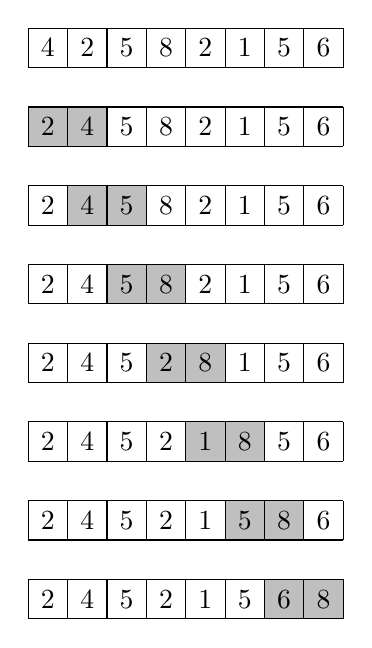
\begin{tikzpicture}[scale=0.5]
\begin{scope}
\draw (0,0) grid (8,1);
\foreach \x/\v in {0/4,1/2,2/5,3/8,4/2,5/1,6/5,7/6} \node at (0.5+\x,0.5) {\v};
\end{scope}
\begin{scope}[yshift=-2cm]
\fill[lightgray] (0,0) rectangle (2,1);
\draw (0,0) grid (8,1);
\foreach \x/\v in {0/2,1/4,2/5,3/8,4/2,5/1,6/5,7/6} \node at (0.5+\x,0.5) {\v};
\end{scope}
\begin{scope}[yshift=-4cm]
\fill[lightgray] (1,0) rectangle (3,1);
\draw (0,0) grid (8,1);
\foreach \x/\v in {0/2,1/4,2/5,3/8,4/2,5/1,6/5,7/6} \node at (0.5+\x,0.5) {\v};
\end{scope}
\begin{scope}[yshift=-6cm]
\fill[lightgray] (2,0) rectangle (4,1);
\draw (0,0) grid (8,1);
\foreach \x/\v in {0/2,1/4,2/5,3/8,4/2,5/1,6/5,7/6} \node at (0.5+\x,0.5) {\v};
\end{scope}
\begin{scope}[yshift=-8cm]
\fill[lightgray] (3,0) rectangle (5,1);
\draw (0,0) grid (8,1);
\foreach \x/\v in {0/2,1/4,2/5,3/2,4/8,5/1,6/5,7/6} \node at (0.5+\x,0.5) {\v};
\end{scope}
\begin{scope}[yshift=-10cm]
\fill[lightgray] (4,0) rectangle (6,1);
\draw (0,0) grid (8,1);
\foreach \x/\v in {0/2,1/4,2/5,3/2,4/1,5/8,6/5,7/6} \node at (0.5+\x,0.5) {\v};
\end{scope}
\begin{scope}[yshift=-12cm]
\fill[lightgray] (5,0) rectangle (7,1);
\draw (0,0) grid (8,1);
\foreach \x/\v in {0/2,1/4,2/5,3/2,4/1,5/5,6/8,7/6} \node at (0.5+\x,0.5) {\v};
\end{scope}
\begin{scope}[yshift=-14cm]
\fill[lightgray] (6,0) rectangle (8,1);
\draw (0,0) grid (8,1);
\foreach \x/\v in {0/2,1/4,2/5,3/2,4/1,5/5,6/6,7/8} \node at (0.5+\x,0.5) {\v};
\end{scope}
\end{tikzpicture}
\caption{Kuplajärjestämisen ensimmäinen kierros.}
\label{fig:kupjar}
\end{figure}


Kuva X näyttää esimerkin kuplajärjestämisen ensimmäisestä
kierroksesta.
Kuplajärjestämisen ominaisuutena on, että $k$ kierroksen
jälkeen taulukon $k$ suurinta alkiota ovat oikeilla paikoillaan
taulukon lopussa.
Niinpä $n$ kierroksen jälkeen koko taulukko on järjestyksessä.

Kuplajärjestämisen voi toteuttaa seuraavalla koodilla:

\begin{code}
for (int i = 0; i < n; i++) {
    for (int j = 0; j < n-1; j++) {
        if (taulu[i] > taulu[j]) {
            swap(taulu[i],taulu[j]);
        }
    }
}
\end{code}

Tässä merkintä \texttt{swap(a,b)} tarkoittaa,
että vaihdamme keskenään arvot \texttt{a} ja \texttt{b}.
Merkintä vastaa siis seuraavaa koodia:

\begin{code}
t = a;
a = b;
b = t;
\end{code}

Kuplajärjestäminen muodostuu $n$ kierroksesta,
joista jokainen käy läpi taulukon,
joten algoritmi vie aikaa $O(n^2)$.

\subsection{Lisäysjärjestäminen}

Lisäysjärjestäminen käy läpi taulukon vasemmalta oikealle
ja siirtää jokaisessa kohdassa olevaa alkiota vasemmalle
niin kauan kuin alkio on pienempi kuin sen vasemmalla
puolella oleva alkio.
Algoritmia voi myös ajatella niin,
että se varmistaa jokaisessa vaiheessa,
että taulukon $k$ ensimmäistä alkiota ovat oikeassa järjestyksessä.

\begin{figure}
\center
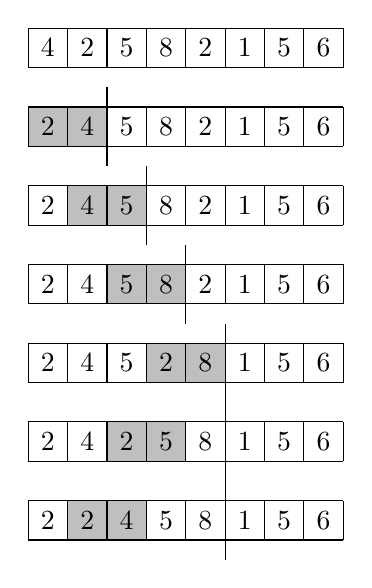
\begin{tikzpicture}[scale=0.5]
\begin{scope}
\draw (0,0) grid (8,1);
\foreach \x/\v in {0/4,1/2,2/5,3/8,4/2,5/1,6/5,7/6} \node at (0.5+\x,0.5) {\v};
\end{scope}
\begin{scope}[yshift=-2cm]
\fill[lightgray] (0,0) rectangle (2,1);
\draw (0,0) grid (8,1);
\foreach \x/\v in {0/2,1/4,2/5,3/8,4/2,5/1,6/5,7/6} \node at (0.5+\x,0.5) {\v};
\draw (2,-0.5) -- (2,1.5);
\end{scope}
\begin{scope}[yshift=-4cm]
\fill[lightgray] (1,0) rectangle (3,1);
\draw (0,0) grid (8,1);
\foreach \x/\v in {0/2,1/4,2/5,3/8,4/2,5/1,6/5,7/6} \node at (0.5+\x,0.5) {\v};
\draw (3,-0.5) -- (3,1.5);
\end{scope}
\begin{scope}[yshift=-6cm]
\fill[lightgray] (2,0) rectangle (4,1);
\draw (0,0) grid (8,1);
\foreach \x/\v in {0/2,1/4,2/5,3/8,4/2,5/1,6/5,7/6} \node at (0.5+\x,0.5) {\v};
\draw (4,-0.5) -- (4,1.5);
\end{scope}
\begin{scope}[yshift=-8cm]
\fill[lightgray] (3,0) rectangle (5,1);
\draw (0,0) grid (8,1);
\foreach \x/\v in {0/2,1/4,2/5,3/2,4/8,5/1,6/5,7/6} \node at (0.5+\x,0.5) {\v};
\draw (5,-0.5) -- (5,1.5);
\end{scope}
\begin{scope}[yshift=-10cm]
\fill[lightgray] (2,0) rectangle (4,1);
\draw (0,0) grid (8,1);
\foreach \x/\v in {0/2,1/4,2/2,3/5,4/8,5/1,6/5,7/6} \node at (0.5+\x,0.5) {\v};
\draw (5,-0.5) -- (5,1.5);
\end{scope}
\begin{scope}[yshift=-12cm]
\fill[lightgray] (1,0) rectangle (3,1);
\draw (0,0) grid (8,1);
\foreach \x/\v in {0/2,1/2,2/4,3/5,4/8,5/1,6/5,7/6} \node at (0.5+\x,0.5) {\v};
\draw (5,-0.5) -- (5,1.5);
\end{scope}
\end{tikzpicture}
\caption{Lisäysjärjestämisen ensimmäiset vaiheet.}
\label{fig:lisjar}
\end{figure}

Kuva \ref{fig:lisjar} näyttää esimerkin,
kuinka lisäysjärjestäminen aloittaa taulukon järjestämisen.
Jokaisessa kohdassa pystyviiva ilmaisee kohdan,
johon päättyy taulukon järjestyksessä oleva alkuosa.
Toisin kuin kuplajärjestämisessä, vierekkäisten alkioiden
vaihtamiset etenevät oikealta vasemmalle.

Seuraava koodi toteuttaa lisäysjärjestämisen:

\begin{code}
for (int i = 1; i < n; i++) {
    int k = i-1;
    while (k >= 0 && taulu[k] > taulu[k+1]) {
        swap(taulu[k],taulu[k+1]);
        k--;
    }
}
\end{code}

\subsection{Inversiot}

Kuplajärjestäminen ja lisäysjärjestäminen ovat esimerkkejä
järjestämis\-algoritmeista, jotka perustuvat vierekkäisten
alkioiden vaihtamiseen.
Osoitamme seuraavaksi, että tällainen algoritmi ei voi koskaan
toimia tehokkaammin kuin ajassa $O(n^2)$.

Hyödyllinen käsite järjestämisalgoritmien analysoinnissa
on \emph{inversio}: kaksi taulukossa olevaa alkiota,
jotka ovat väärässä järjestyksessä.
Tässä otetaan huomioon kaikki taulukon alkioparit,
ei vain vierekkäin olevia alkioita.
Esimerkiksi taulukossa $[3,1,4,2]$ on kolme inversiota:
$(3,1)$, $(3,2)$ ja $(4,2)$.

Taulukon inversioiden määrä kertoo, miten paljon työtä
vaaditaan sen järjestämiseen. Jos inversioiden määrä on 0,
taulukko on järjestyksessä.
Jos taas taulukko on käänteisessä järjestyksessä
suurimmasta pienimpään, sen inversioiden määrä on
\[
(n-1) + (n-2) + \dots + 1 = \frac{n(n-1)}{2} = O(n^2).
\]

Aina kun vaihdamme taulukossa kahden vierekkäin olevan
alkion järjes\-tyksen, saamme poistettua taulukosta enintään
yhden inversion.
Niinpä jos taulukossa on $O(n^2)$ inversiota,
mikä tahansa vierekkäisiä alkioita vaihtava algoritmi
käyttää sen järjestämiseen aikaa ainakin $O(n^2)$.
Emme siis koskaan pysty luomaan tehokasta järjestämisalgoritmia,
jos keskitymme vain algoritmeihin, jotka vaihtavat
keskenään vierekkäisiä alkioita.

\subsection{Vaihtojärjestäminen}

Vaihtojärjestäminen etsii ensin taulukon pienimmän alkion
ja vaihtaa sen ensimmäiseksi.
Tämän jälkeen se käsittelee vastaavasti taulukon
jäljellä olevan osan, jne., kunnes taulukko on järjestyksessä.
Kuva \ref{fig:vaijar} näyttää esimerkin
vaihtojärjestämisen toiminnasta.

\begin{figure}
\center
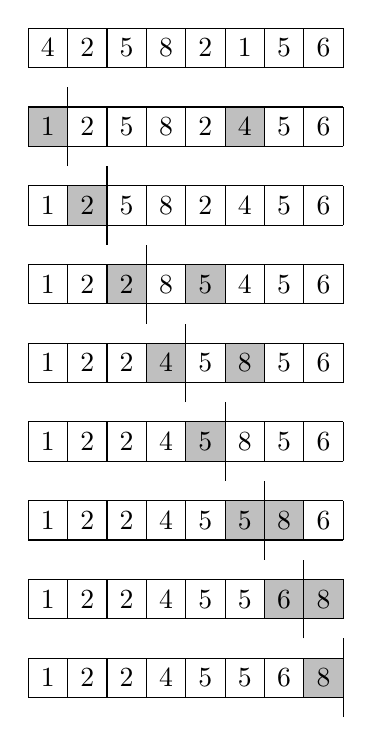
\begin{tikzpicture}[scale=0.5]
\begin{scope}
\draw (0,0) grid (8,1);
\foreach \x/\v in {0/4,1/2,2/5,3/8,4/2,5/1,6/5,7/6} \node at (0.5+\x,0.5) {\v};
\end{scope}
\begin{scope}[yshift=-2cm]
\fill[lightgray] (0,0) rectangle (1,1);
\fill[lightgray] (5,0) rectangle (6,1);
\draw (0,0) grid (8,1);
\foreach \x/\v in {0/1,1/2,2/5,3/8,4/2,5/4,6/5,7/6} \node at (0.5+\x,0.5) {\v};
\draw (1,-0.5) -- (1,1.5);
\end{scope}
\begin{scope}[yshift=-4cm]
\fill[lightgray] (1,0) rectangle (2,1);
\fill[lightgray] (1,0) rectangle (2,1);
\draw (0,0) grid (8,1);
\foreach \x/\v in {0/1,1/2,2/5,3/8,4/2,5/4,6/5,7/6} \node at (0.5+\x,0.5) {\v};
\draw (2,-0.5) -- (2,1.5);
\end{scope}
\begin{scope}[yshift=-6cm]
\fill[lightgray] (2,0) rectangle (3,1);
\fill[lightgray] (4,0) rectangle (5,1);
\draw (0,0) grid (8,1);
\foreach \x/\v in {0/1,1/2,2/2,3/8,4/5,5/4,6/5,7/6} \node at (0.5+\x,0.5) {\v};
\draw (3,-0.5) -- (3,1.5);
\end{scope}
\begin{scope}[yshift=-8cm]
\fill[lightgray] (3,0) rectangle (4,1);
\fill[lightgray] (5,0) rectangle (6,1);
\draw (0,0) grid (8,1);
\foreach \x/\v in {0/1,1/2,2/2,3/4,4/5,5/8,6/5,7/6} \node at (0.5+\x,0.5) {\v};
\draw (4,-0.5) -- (4,1.5);
\end{scope}
\begin{scope}[yshift=-10cm]
\fill[lightgray] (4,0) rectangle (5,1);
\fill[lightgray] (4,0) rectangle (5,1);
\draw (0,0) grid (8,1);
\foreach \x/\v in {0/1,1/2,2/2,3/4,4/5,5/8,6/5,7/6} \node at (0.5+\x,0.5) {\v};
\draw (5,-0.5) -- (5,1.5);
\end{scope}
\begin{scope}[yshift=-12cm]
\fill[lightgray] (5,0) rectangle (6,1);
\fill[lightgray] (6,0) rectangle (7,1);
\draw (0,0) grid (8,1);
\foreach \x/\v in {0/1,1/2,2/2,3/4,4/5,5/5,6/8,7/6} \node at (0.5+\x,0.5) {\v};
\draw (6,-0.5) -- (6,1.5);
\end{scope}
\begin{scope}[yshift=-14cm]
\fill[lightgray] (6,0) rectangle (7,1);
\fill[lightgray] (7,0) rectangle (8,1);
\draw (0,0) grid (8,1);
\foreach \x/\v in {0/1,1/2,2/2,3/4,4/5,5/5,6/6,7/8} \node at (0.5+\x,0.5) {\v};
\draw (7,-0.5) -- (7,1.5);
\end{scope}
\begin{scope}[yshift=-16cm]
\fill[lightgray] (7,0) rectangle (8,1);
\fill[lightgray] (7,0) rectangle (8,1);
\draw (0,0) grid (8,1);
\foreach \x/\v in {0/1,1/2,2/2,3/4,4/5,5/5,6/6,7/8} \node at (0.5+\x,0.5) {\v};
\draw (8,-0.5) -- (8,1.5);
\end{scope}
\end{tikzpicture}
\caption{Esimerkki vaihtojärjestämisen toiminnasta.}
\label{fig:vaijar}
\end{figure}


Seuraava koodi toteuttaa vaihtojärjestämisen:

\begin{code}
for (int i = 0; i < n; i++) {
    int k = i;
    for (int j = i; j < n; j++) {
        if (taulu[j] < taulu[k]) k = j;
    }
    swap(taulu[i],taulu[k]);
}
\end{code}

Toisin kuin kuplajärjestäminen ja lisäysjärjestäminen,
vaihtojärjestäminen vaihtaa vain $O(n)$ alkiota keskenään
taulukossa, koska se siirtää aina pienimmän alkion
suoraan oikeaan kohtaan.
Algoritmi vie kuitenkin $O(n^2)$ aikaa,
koska jokaisen pienimmän alkion löytäminen vie $O(n)$ aikaa.

Myöhemmin luvussa X huomaamme kuitenkin,
että voimme luoda vaihtojärjestämisen idealla tehokkaan
$O(n \log n)$-algoritmin käyttämällä apuna kekorakennetta.

\section{Tehokkaat algoritmit}

\subsection{Lomitusjärjestäminen}

\subsection{Pikajärjestäminen}

\subsection{Järjestämisen alaraja}

\subsection{Laskemisjärjestäminen}

\section{Järjestäminen Javassa}

Käytännössä ei ole yleensä hyvä idea toteuttaa itse
järjestämisalgoritmia, koska nykypäivän ohjelmointikielissä
on valmiit työkalut järjestämiseen.
Esimerkiksi Javassa voimme käyttää metodia \texttt{Arrays.sort},
joka järjestää sille annetun taulukon:

\begin{code}
int[] taulu = {4,2,5,8,2,1,5,6};
Arrays.sort(taulu);
\end{code}

Kiinnostava kysymys on, mitä algoritmia Java käyttää
taulukon järjes\-tämiseen.
Yllättävää kyllä, tämä riippuu siitä, minkä tyyppistä tietoa
taulukossa on.
Jos taulukon alkiot ovat alkeistyyppisiä
(esimerkiksi \texttt{int}), Java käyttää 
pikajärjestämisen muunnelmaa.
Jos taas alkiot ovat oliotyyppisiä
(esimerkiksi \texttt{String}),
algoritmina on lomitusjärjestäminen.

Jos haluamme, että Java pystyy järjestämään omia olioitamme,
meidän täytyy toteuttaa luokkaan metodi \texttt{compareTo} ja
merkitä, että luokka toteuttaa rajapinnan \texttt{Comparable}.
Kun \texttt{Arrays.sort} järjestää taulukon,
se kutsuu metodia \texttt{compareTo} aina, kun se haluaa selvittää
kahden alkion suuruusjärjestyksen.
Metodin tulee palauttaa negatiivinen arvo, nolla tai positiivinen arvo
sen mukaan, onko olio itse pienempi, yhtä suuri vai suurempi
kuin parametrina annettu olio.

Esimerkiksi seuraava koodi toteuttaa luokan \texttt{Piste},
johon voidaan tallentaa pisteen x- ja y-koordinaatit.
Luokassa on metodi \texttt{compareTo}, joka määrittelee,
että pisteet järjestetään ensisijaisesti x-koordinaatin ja
toissijaisesti y-koordinaatin mukaan.

\begin{code}
public class Piste implements Comparable<Piste> {
    public int x, y;

    public int compareTo(Piste p) {
        if (this.x != p.x) return this.x-p.x;
        else return this.y-p.y;
    }
}
\end{code}

Metodin \texttt{compareTo} avulla voimme myös konkreettisesti
tarkastella, mitä Java tekee järjestäessään taulukon.
Seuraava luokka sisältää vain yhden luvun,
mutta ilmoittaa meille aina, kun Java kutsuu
\texttt{compareTo}-funktiota:

\begin{code}
public class Luku implements Comparable<Luku> {
    public int luku;

    public int compareTo(Luku x) {
        System.out.println("vertailu: " + luku + " " + x.luku);
        return this.luku-x.luku;
    }
}
\end{code}

Esimerkiksi kun järjestettävänä taulukkona on $[4,1,3,2]$,
saamme tietää, että Java tekee seuraavat vertailut:

\begin{code}
vertailu: 1 4
vertailu: 3 1
vertailu: 3 4
vertailu: 3 1
vertailu: 2 3
vertailu: 2 1
\end{code}

\section{Esimerkkejä}

\chapter{Lista}

\emph{Lista} on tietorakenne,
joka muodostuu peräkkäin olevista alkioista.
Esimerkiksi $[3,7,2,5]$ on lista,
joka sisältää neljä alkiota.
Merkitsemme listan alkioiden määrää
kirjaimella $n$ ja indeksoimme alkiot
$0,1,\dots,n-1$.
Haluamme toteuttaa listan niin,
että pääsemme käsiksi tietyssä kohdassa
olevaan alkioon sekä pystymme
lisäämään ja poistamaan alkioita.

Tässä luvussa tutustumme kahteen
tapaan listan luomiseen.
Ensin toteutamme taulukkolistan,
jossa listan alkiot tallennetaan taulukkoon.
Tämän jälkeen toteutamme linkitetyn listan,
joka muodostuu toisiinsa viittaavista solmuista.
Kuten tulemme huomaamaan, molemmissa listan toteutuksissa on omat
hyvät ja huonot puolensa.

\section{Taulukkolista}

\emph{Taulukkolista} on lista, joka on tallennettu taulukkona.
Koska taulukon alkiot sijaitsevat aina peräkkäin muistissa,
pääsemme käsiksi mihin tahansa listan alkioon ajassa $O(1)$.
Toisaalta haasteena toteutuksessa on,
että taulukon koko on \emph{kiinteä} ja jos haluamme
muuttaa kokoa, meidän täytyy varata uusi taulukko
ja kopioida sinne vanhan taulukon sisältö.

\subsection{Muutokset lopussa}

Toteutamme ensin taulukkolistan, jossa alkioiden
lisäykset ja poistot tapahtuvat listan lopussa.
Tallennamme listan taulukkona niin,
että tietty määrä alkioita taulukon alussa on listan käytössä
ja loput tyhjät kohdat on varattu tuleville alkioille.
Tämän ansiosta pystymme lisäämään uuden alkion listalle
ajassa $O(1)$, jos taulukossa on tilaa,
koska meidän riittää ottaa käyttöön seuraava
vapaana oleva kohta taulukosta.

Kuva \ref{fig:listau} näyttää esimerkin,
jossa taulukossa on tilaa yhteenä kahdeksalle alkiolle
ja siihen on tallennettu lista $[3,7,2,5]$.
Taulukon neljä ensimmäistä alkiota ovat siis listan käytössä
ja muut ovat varalla tulevia alkioita varten.
Kun lisäämme listan loppuun uuden alkion 6,
otamme käyttöön taulukosta uuden kohdan, johon alkio sijoitetaan.

\begin{figure}
\center
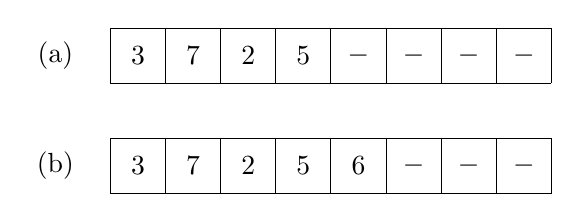
\begin{tikzpicture}[scale=0.7]
\begin{scope}
\draw (0,0) grid (8,1);
\node at (-1,0.5) {(a)};
\node at (0.5,0.5) {$3$};
\node at (1.5,0.5) {$7$};
\node at (2.5,0.5) {$2$};
\node at (3.5,0.5) {$5$};
\node at (4.5,0.5) {$-$};
\node at (5.5,0.5) {$-$};
\node at (6.5,0.5) {$-$};
\node at (7.5,0.5) {$-$};
\end{scope}
\begin{scope}[yshift=-2cm]
\draw (0,0) grid (8,1);
\node at (-1,0.5) {(b)};
\node at (0.5,0.5) {$3$};
\node at (1.5,0.5) {$7$};
\node at (2.5,0.5) {$2$};
\node at (3.5,0.5) {$5$};
\node at (4.5,0.5) {$6$};
\node at (5.5,0.5) {$-$};
\node at (6.5,0.5) {$-$};
\node at (7.5,0.5) {$-$};
\end{scope}
\end{tikzpicture}
\caption{(a) Lista $[3,7,2,5]$ tallennettuna taulukkoon. (b) Listan loppuun lisätään alkio 6.}
\label{fig:listau}
\end{figure}

\begin{figure}
\center
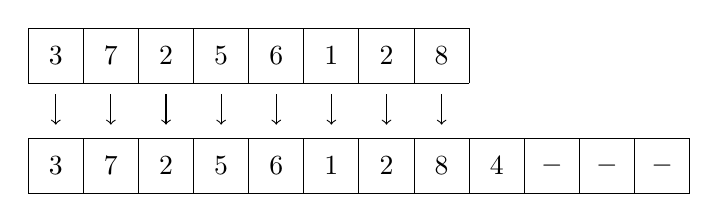
\begin{tikzpicture}[scale=0.7]
\begin{scope}
\draw (0,0) grid (8,1);
\node at (0.5,0.5) {$3$};
\node at (1.5,0.5) {$7$};
\node at (2.5,0.5) {$2$};
\node at (3.5,0.5) {$5$};
\node at (4.5,0.5) {$6$};
\node at (5.5,0.5) {$1$};
\node at (6.5,0.5) {$2$};
\node at (7.5,0.5) {$8$};
\foreach \x in {0,...,7} \draw[->] (\x+0.5,-0.2) -- (\x+0.5,-0.75);
\end{scope}
\begin{scope}[yshift=-2cm]
\draw (0,0) grid (12,1);
\node at (0.5,0.5) {$3$};
\node at (1.5,0.5) {$7$};
\node at (2.5,0.5) {$2$};
\node at (3.5,0.5) {$5$};
\node at (4.5,0.5) {$6$};
\node at (5.5,0.5) {$1$};
\node at (6.5,0.5) {$2$};
\node at (7.5,0.5) {$8$};
\node at (8.5,0.5) {$4$};
\node at (9.5,0.5) {$-$};
\node at (10.5,0.5) {$-$};
\node at (11.5,0.5) {$-$};
\end{scope}
\end{tikzpicture}
\caption{Taulukkoon ei mahdu enää uutta alkiota. Meidän täytyy varata uusi suurempi taulukko
ja kopioida vanhan taulukon sisältö sinne.}
\label{fig:lisuus}
\end{figure}

Mitä tapahtuu sitten, kun jossain vaiheessa koko taulukko
on täynnä eikä uusi listalle lisättävä alkio mahdu enää taulukkoon?
Tällöin meidän täytyy ensin varata uusi suurempi taulukko ja
kopioida kaikki vanhan taulukon alkiot siihen.
Vasta tämän jälkeen voimme lisätä uuden alkion listalle.
Tämä vie aikaa $O(n)$, koska kopioimme kaikki listan alkiot
uuteen paikkaan muistissa.
Esimerkiksi kuvassa \ref{fig:lisuus} uusi alkio 4 ei mahdu taulukkoon,
joten joudumme varaamaan uuden taulukon ja kopioimaan alkiot.

Olemme saaneet siis aikaan listan, jossa lisääminen
vie aikaa \emph{joko} $O(1)$ tai $O(n)$ riippuen siitä,
mahtuuko alkio nykyiseen taulukkoon vai täytyykö
meidän varata uusi taulukko.
Jotta lista olisi käyttökelpoinen, hidas $O(n)$-operaatio
ei saisi esiintyä liian usein.
Osoittautuu, että saavutamme tämän tavoitteen,
kunhan varaamme uuden taulukon aina reilusti aiempaa suuremmaksi.
Tavanomainen ratkaisu on \emph{kaksinkertaistaa} taulukon koko aina,
kun varaamme uuden taulukon.
Kun toimimme näin, jokaisen alkion lisääminen listalle vie
\emph{keskimäärin} vain $O(1)$ aikaa.

Voimme ajatella asian näin: jokainen listalle lisättävä alkio
maksaa \emph{pääsy\-maksuna} kolme euroa.
Tästä yksi euro menee listalle liittymiseen ja kaksi euroa jäävät säästöön.
Sitten kun aikanaan listalle täytyy varata suurempi taulukko,
jokainen viime erässä lisätty alkio maksaa yhden euron omasta siirrostaan
ja yhden euron aiemmin lisätyn alkion siirrosta.
Koska taulukon koko kaksinkertaistuu joka vaiheessa,
kolmen euron kiinteä pääsymaksu riittää siihen, että kaikki tulevat
siirrot saadaan kustannettua.

\begin{figure}
\center
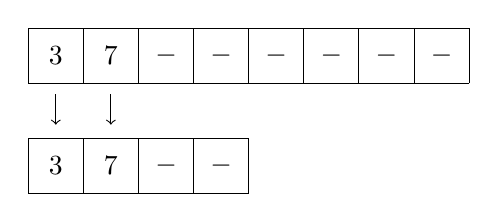
\begin{tikzpicture}[scale=0.7]
\begin{scope}
\draw (0,0) grid (8,1);
\node at (0.5,0.5) {$3$};
\node at (1.5,0.5) {$7$};
\node at (2.5,0.5) {$-$};
\node at (3.5,0.5) {$-$};
\node at (4.5,0.5) {$-$};
\node at (5.5,0.5) {$-$};
\node at (6.5,0.5) {$-$};
\node at (7.5,0.5) {$-$};
\foreach \x in {0,...,1} \draw[->] (\x+0.5,-0.2) -- (\x+0.5,-0.75);
\end{scope}
\begin{scope}[yshift=-2cm]
\draw (0,0) grid (4,1);
\node at (0.5,0.5) {$3$};
\node at (1.5,0.5) {$7$};
\node at (2.5,0.5) {$-$};
\node at (3.5,0.5) {$-$};
\end{scope}
\end{tikzpicture}
\caption{Poistojen jälkeen taulukon koko on käynyt tarpeettoman suureksi,
ja puolitamme taulukon koon.}                                                                        
\label{fig:lispoi}
\end{figure}

Voimme poistaa alkion listan lopusta aina $O(1)$-ajassa,
koska taulukon kokoa ei tarvitse koskaan suurentaa.
Tässä voisi kuitenkin tulla ongelmaksi, että monien poistojen
jälkeen taulukossa olisi turhan paljon tyhjää tilaa lopussa.
Voimme soveltaa tässä käänteisesti samaa ideaa kuin lisäämisessä:
jos poistamisen jälkeen vain \emph{neljännes} taulukosta on käytössä,
puolitamme taulukon koon.
Kuva \ref{fig:lispoi} näyttää esimerkin tällaisesta tilanteesta.
Tällä tavalla myös poistamiset vievät keskimäärin aikaa $O(1)$.

Miksi emme voisi varata heti aluksi niin suurta taulukkoa,
että lopullinen lista mahtuisi siihen varmasti?
Tässä olisi huonona puolena, että listamme tuhlaisi paljon muistia.
Algoritmissa saattaa olla samaan aikaan käytössä monia listoja,
ja haluamme, että listalle varattu taulukko on samaa kokoluokkaa
kuin listan todellinen sisältö.

\subsection{Muutokset alussa ja lopussa}

Melko samaan tapaan voimme myös luoda taulukkolistan,
joka sallii tehokkaat alkioiden lisäykset ja poistot
sekä listan alussa että lopussa.
Jotta tämä onnistuisi, muutamme listan tallennustapaa niin,
että lista voi alkaa ja päättyä missä tahansa taulukon
kohdassa ja listan sisältö voi tarvittaessa jatkua taulukon lopusta alkuun.

\begin{figure}
\center
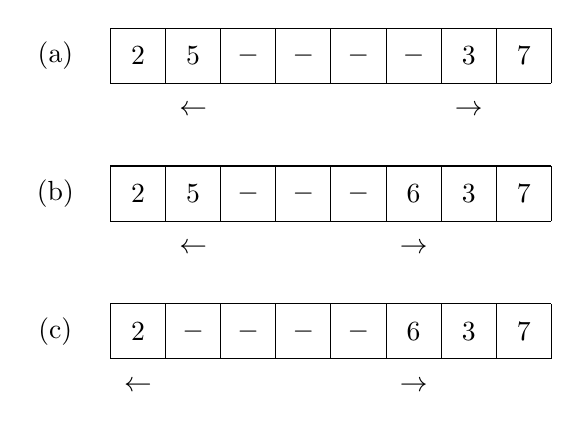
\begin{tikzpicture}[scale=0.7]
\begin{scope}
\draw (0,0) grid (8,1);
\node at (-1,0.5) {(a)};
\node at (0.5,0.5) {$2$};
\node at (1.5,0.5) {$5$};
\node at (2.5,0.5) {$-$};
\node at (3.5,0.5) {$-$};
\node at (4.5,0.5) {$-$};
\node at (5.5,0.5) {$-$};
\node at (6.5,0.5) {$3$};
\node at (7.5,0.5) {$7$};
\node at (1.5,-0.5) {$\leftarrow$};
\node at (6.5,-0.5) {$\rightarrow$};
\end{scope}
\begin{scope}[yshift=-2.5cm]
\draw (0,0) grid (8,1);
\node at (-1,0.5) {(b)};
\node at (0.5,0.5) {$2$};
\node at (1.5,0.5) {$5$};
\node at (2.5,0.5) {$-$};
\node at (3.5,0.5) {$-$};
\node at (4.5,0.5) {$-$};
\node at (5.5,0.5) {$6$};
\node at (6.5,0.5) {$3$};
\node at (7.5,0.5) {$7$};
\node at (1.5,-0.5) {$\leftarrow$};
\node at (5.5,-0.5) {$\rightarrow$};
\end{scope}
\begin{scope}[yshift=-5cm]
\draw (0,0) grid (8,1);
\node at (-1,0.5) {(c)};
\node at (0.5,0.5) {$2$};
\node at (1.5,0.5) {$-$};
\node at (2.5,0.5) {$-$};
\node at (3.5,0.5) {$-$};
\node at (4.5,0.5) {$-$};
\node at (5.5,0.5) {$6$};
\node at (6.5,0.5) {$3$};
\node at (7.5,0.5) {$7$};
\node at (0.5,-0.5) {$\leftarrow$};
\node at (5.5,-0.5) {$\rightarrow$};
\end{scope}
\end{tikzpicture}
\caption{(a) Lista $[3,7,2,5]$ tallennettuna taulukkoon.
(b) Listan alkuun lisätään alkio 6.
(c) Listan lopusta poistetaan alkio 5.}
\label{fig:lismol}
\end{figure}

Kuva \ref{fig:lismol} näyttää esimerkin listan $[3,7,2,5]$
uudesta tallennustavasta.
Merkki $\rightarrow$ osoittaa kohdan, josta lista alkaa,
ja merkki $\leftarrow$ osoittaa kohdan, johon lista päättyy.
Kun haluamme lisätä alkion listan alkuun,
siirrymme vasemmalle kohdasta $\rightarrow$,
ja kun haluamme lisätä alkion listan loppuun,
siirrymme oikealle kohdasta $\leftarrow$.
Kun haluamme poistaa alkioita listasta,
menettelemme käänteisesti.

\begin{figure}
\center
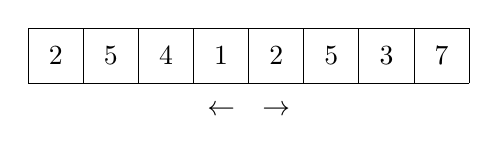
\begin{tikzpicture}[scale=0.7]
\begin{scope}
\draw (0,0) grid (8,1);
\node at (0.5,0.5) {$2$};
\node at (1.5,0.5) {$5$};
\node at (2.5,0.5) {$4$};
\node at (3.5,0.5) {$1$};
\node at (4.5,0.5) {$2$};
\node at (5.5,0.5) {$5$};
\node at (6.5,0.5) {$3$};
\node at (7.5,0.5) {$7$};
\node at (3.5,-0.5) {$\leftarrow$};
\node at (4.5,-0.5) {$\rightarrow$};
\end{scope}
\end{tikzpicture}
\caption{Lista $[2,5,3,7,2,5,4,1]$ täyttää koko taulukon, emmekä voi lisätä uutta alkiota.
Ratkaisuna on varata suurempi taulukko.}
\label{fig:lismol2}
\end{figure}

Jos kohdat $\rightarrow$ ja $\leftarrow$ ovat vierekkäin,
taulukko on täynnä, emmekä voi enää lisätä uutta alkiota
listan alkuun tai loppuun.
Kuva \ref{fig:lismol2} näyttää esimerkin tällaisesta tilanteesta.
Tällöin meidän täytyy varata uusi suurempi taulukko,
johon listan sisältö siirretään.
Voimme menetellä samalla tavalla kuin aiemmin ja
kaksinkertaistaa taulukon koon joka vaiheessa,
jolloin operaatiot vievät keskimäärin aikaa $O(1)$.

\section{Linkitetty lista}

\emph{Linkitetty lista} muodostuu solmuista, joista jokainen sisältää
yhden listan alkion.
Linkitetty lista voi olla yhteen tai kahteen suuntaan linkitetty.
Yhteen suuntaan linkitetyssä listassa jokaisesta solmusta
on viittaus seuraavaan solmuun, ja kahteen suuntaan linkitetyssä
listassa jokaisesta solmusta on viittaus sekä seuraavaan että edelliseen solmuun.

\begin{figure}
\center
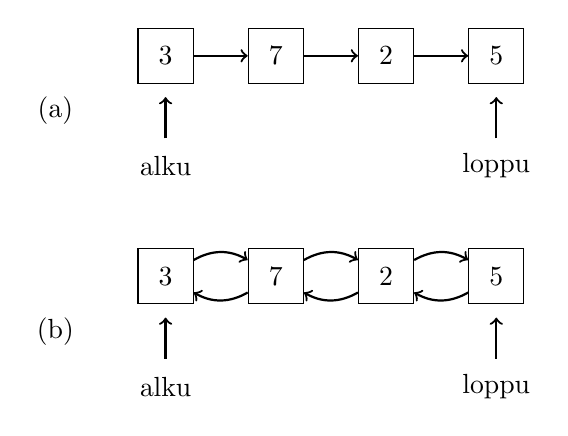
\begin{tikzpicture}[scale=0.7]
\begin{scope}
\node[draw, rectangle, minimum size=7mm] (1) at (0,0) {$3$};
\node[draw, rectangle, minimum size=7mm] (2) at (2,0) {$7$};
\node[draw, rectangle, minimum size=7mm] (3) at (4,0) {$2$};
\node[draw, rectangle, minimum size=7mm] (4) at (6,0) {$5$};
\path[draw,thick,->] (1) -- (2);
\path[draw,thick,->] (2) -- (3);
\path[draw,thick,->] (3) -- (4);
\node at (0,-2) {alku};
\node at (6,-2) {loppu};
\path[draw,thick,->] (0,-1.5) -- (0,-0.75);
\path[draw,thick,->] (6,-1.5) -- (6,-0.75);
\node at (-2,-1) {(a)};
\end{scope}
\begin{scope}[yshift=-4cm]
\node[draw, rectangle, minimum size=7mm] (1) at (0,0) {$3$};
\node[draw, rectangle, minimum size=7mm] (2) at (2,0) {$7$};
\node[draw, rectangle, minimum size=7mm] (3) at (4,0) {$2$};
\node[draw, rectangle, minimum size=7mm] (4) at (6,0) {$5$};
\path[draw,thick,->] (1) edge [bend left] (2);
\path[draw,thick,->] (2) edge [bend left] (3);
\path[draw,thick,->] (3) edge [bend left] (4);
\path[draw,thick,->] (4) edge [bend left] (3);
\path[draw,thick,->] (3) edge [bend left] (2);
\path[draw,thick,->] (2) edge [bend left] (1);
\node at (0,-2) {alku};
\node at (6,-2) {loppu};
\path[draw,thick,->] (0,-1.5) -- (0,-0.75);
\path[draw,thick,->] (6,-1.5) -- (6,-0.75);
\node at (-2,-1) {(b)};
\end{scope}
\end{tikzpicture}
\caption{Lista $[3,7,2,5]$ linkitettynä listana.
(a) Yhteen suuntaan linkitetty lista. (b) Kahteen suuntaan linkitetty lista.}
\label{fig:linlis}
\end{figure}

Kuva \ref{fig:linlis} näyttää esimerkkinä listan $[3,7,2,5]$
yhteen ja kahteen suuntaan linkitettynä.
Molemmissa listoissa tiedossamme on viittaukset listan
alkuun ja loppuun.
Yhteen suuntaan linkitetyssä listassa voimme käydä
läpi listan alkiot alusta loppuun,
kun taas kahteen suuntaan linkitetyssä listassa
voimme liikkua sekä alusta loppuun että lopusta alkuun.

Kaksisuuntainen linkitys on käytännössä järkevä tapa toteuttaa
linkitetty lista, ja oletamme jatkossa, että listamme on
kahteen suuntaan linkitetty ja meillä on tiedossa viittaukset
listan alkuun ja loppuun.

\subsection{Linkitetyt rakenteet}

Jokaisessa ohjelmointikielessä on omat keinonsa
linkitetyn rakenteen toteuttamiseen.
Javassa voimme toteuttaa linkitetyn rakenteen niin,
että jokainen solmu on oma olionsa.
Esimerkiksi voimme toteuttaa seuraavan luokan \texttt{Solmu},
jonka oliot toimivat linkitetyn listan solmuina:

\begin{code}
public class Solmu {
    public int arvo;
    public Solmu seuraava;
    public Solmu edellinen;

    public Solmu(int arvo, Solmu seuraava, Solmu edellinen) {
        this.arvo = arvo;
        this.seuraava = seuraava;
        this.edellinen = edellinen;
    }
}
\end{code}

Kenttä \texttt{arvo} kertoo solmun arvon,
kenttä \texttt{seuraava} osoittaa seuraavaan solmuun
ja kenttä \texttt{edellinen} osoittaa edelliseen solmuun.
Jos seuraavaa tai edellistä solmua ei ole,
viittauksen tilalla on arvo \texttt{null}.
Tämän luokan avulla voisimme luoda linkitetyn listan $[3,7,2,5]$
seuraavasti:

\begin{code}
Solmu s1, s2, s3, s4;
s1 = new Solmu(3, s2, null);
s2 = new Solmu(7, s3, s1);
s3 = new Solmu(2, s4, s2);
s4 = new Solmu(5, null, s3);
\end{code}

Tämän jälkeen voisimme käydä listan läpi näin alusta loppuun:

\begin{code}
Solmu s = s1;
while (s != null) {
    System.out.println(s.arvo);
    s = s.seuraava;
}
\end{code}

Koodin tulostus on seuraava:

\begin{code}
3
7
2
5
\end{code}

\subsection{Listan operaatiot}

Linkitetyn listan etuna on,
että voimme lisätä ja poistaa
alkioita $O(1)$-ajassa kaikissa listan kohdissa.
Kun haluamme lisätä listalle alkion,
luomme ensin uuden solmun ja muutamme sitten
sen vieressä olevien solmujen viittauksia niin,
että ne viittaavat uuteen solmuun.
Vastaavasti kun haluamme poistaa alkion,
muutamme viittauksia niin, että solmu ohitetaan.

\begin{figure}
\center
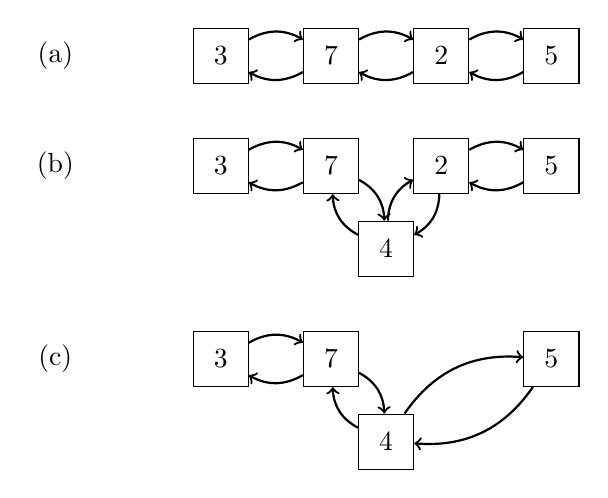
\begin{tikzpicture}[scale=0.7]
\begin{scope}
\node at (-3,0) {(a)};
\node[draw, rectangle, minimum size=7mm] (1) at (0,0) {$3$};
\node[draw, rectangle, minimum size=7mm] (2) at (2,0) {$7$};
\node[draw, rectangle, minimum size=7mm] (3) at (4,0) {$2$};
\node[draw, rectangle, minimum size=7mm] (4) at (6,0) {$5$};
\path[draw,thick,->] (1) edge [bend left] (2);
\path[draw,thick,->] (2) edge [bend left] (3);
\path[draw,thick,->] (3) edge [bend left] (4);
\path[draw,thick,->] (4) edge [bend left] (3);
\path[draw,thick,->] (3) edge [bend left] (2);
\path[draw,thick,->] (2) edge [bend left] (1);
\end{scope}
\begin{scope}[yshift=-2cm]
\node at (-3,0) {(b)};
\node[draw, rectangle, minimum size=7mm] (1) at (0,0) {$3$};
\node[draw, rectangle, minimum size=7mm] (2) at (2,0) {$7$};
\node[draw, rectangle, minimum size=7mm] (3) at (4,0) {$2$};
\node[draw, rectangle, minimum size=7mm] (4) at (6,0) {$5$};
\node[draw, rectangle, minimum size=7mm] (5) at (3,-1.5) {$4$};
\path[draw,thick,->] (1) edge [bend left] (2);
\path[draw,thick,->] (2) edge [bend left] (5);
\path[draw,thick,->] (5) edge [bend left] (3);
\path[draw,thick,->] (3) edge [bend left] (4);
\path[draw,thick,->] (4) edge [bend left] (3);
\path[draw,thick,->] (3) edge [bend left] (5);
\path[draw,thick,->] (5) edge [bend left] (2);
\path[draw,thick,->] (2) edge [bend left] (1);
\end{scope}
\begin{scope}[yshift=-5.5cm]
\node at (-3,0) {(c)};
\node[draw, rectangle, minimum size=7mm] (1) at (0,0) {$3$};
\node[draw, rectangle, minimum size=7mm] (2) at (2,0) {$7$};
\node[draw, rectangle, minimum size=7mm] (4) at (6,0) {$5$};
\node[draw, rectangle, minimum size=7mm] (5) at (3,-1.5) {$4$};
\path[draw,thick,->] (1) edge [bend left] (2);
\path[draw,thick,->] (2) edge [bend left] (5);
\path[draw,thick,->] (5) edge [bend left] (4);
\path[draw,thick,->] (4) edge [bend left] (5);
\path[draw,thick,->] (5) edge [bend left] (2);
\path[draw,thick,->] (2) edge [bend left] (1);
\end{scope}
\end{tikzpicture}
\caption{(a) Alkuperäinen lista $[3,7,2,5]$.
(b) Listan keskelle lisätään alkio $4$.
(c) Listasta poistetaan alkio $2$.}
\label{fig:lismuu}
\end{figure}

Kuva \ref{fig:lismuu} näyttää esimerkin linkitetyn listan käsittelystä.
Listan sisältönä on aluksi $[3,7,2,5]$.
Sitten lisämme listan keskelle alkion 4,
jolloin luomme ensin uuden solmun alkiolle ja muutamme
sitten viittauksia alkioiden 7 ja 2 välillä niin,
että alkio 4 tulee niiden väliin.
Lopuksi poistamme listasta alkion 2, jolloin yhdistämme
alkiot 4 ja 5 suoraan toisiinsa.

Pääsemme listan ensimmäiseen ja viimeiseen solmuun tehokkaasti,
koska meillä on muistissa viittaukset niihin.
Sen sijaan jos haluamme päästä johonkin muuhun listan kohtaan,
meidän täytyy aloittaa listan alusta tai lopusta ja kulkea askel
kerrallaan viittauksia seuraten.
Niinpä listan keskellä olevaan kohtaan pääseminen vie aikaa $O(n)$.
Joudumme liikkumaan solmuihin linkkejä pitkin, koska solmut voivat
olla eri puolilla muistia eikä meillä ole keinoa tietää suoraan,
mihin mikäkin solmu on tallennettu.

\subsection{Listojen vertailua}

\begin{table}
\center
\begin{tabular}{lrr}
operaatio & taulukkolista & linkitetty lista \\
\hline
pääsy listan alkuun & $O(1)$ & $O(1)$ \\
pääsy listan loppuun & $O(1)$ & $O(1)$ \\ 
pääsy listan keskelle &  $O(1)$ & $O(n)$ \\
lisäys/poisto listan alussa & $O(1)^*$ & $O(1)$ \\
lisäys/poisto listan lopussa & $O(1)^*$ & $O(1)$ \\ 
lisäys/poisto listan keskellä &  $O(n)$ & $O(1)$ \\
\end{tabular}
\caption{Taulukkolistan ja linkitetyn listan operaatioiden
aikavaativuuksia. Merkintä $^*$ tarkoittaa keskimääräistä aikavaativuutta.}
\label{tab:taulin}
\end{table}

Taulukko \ref{tab:taulin} esittää yhteenvedon taulukkolistan ja
linkitetyn listan ominaisuuksista.
Kummassakin toteutuksessa on yksi operaatio,
joka ei ole tehokas.
Taulukkolistassa pääsemme tehokkaasti mihin tahansa listan
kohtaan, mutta on hidasta muokata listaa keskeltä.
Linkitetyssä listassa voimme muokata listaa mistä tahansa,
mutta keskelle pääseminen on hidasta.

Huomaa, että keskelle pääsemisen hitaus rajoittaa melko paljon
linkitetyn listan käyttämistä.
Vaikka pystymme sinänsä muokkaamaan listaa mistä tahansa kohdasta
tehokkaasti, meidän tulee ensin \emph{päästä} kyseiseen kohtaan.
Jos meillä on jostain syystä etukäteen tiedossa viittaus listan keskelle,
voimme muokata kyseistä kohtaa tehokkaasti,
mutta muuten meidän tulee ensin kulkea haluttuun kohtaan,
missä kuluu aikaa $O(n)$.

\section{Pino ja jono}

Listan avulla voimme toteuttaa myös kaksi erikoistunutta tietorakennetta,
pinon ja jonon, jotka sisältävät vain osan listan ominaisuuksista
eli niiden operaatiot ovat listaa rajoittuneempia.

\emph{Pino} on tietorakenne, jossa on kolme operaatiota:
alkion lisääminen pinon päälle, ylimmän alkion hakeminen
sekä ylimmän alkion poistaminen.
Pystymme siis käsittelemään vain pinon ylintä alkiota.
Voimme toteuttaa pinon helposti listan avulla niin,
että kaikki operaatiot vievät aikaa $O(1)$.

\emph{Jono} on puolestaan tietorakenne, jossa voimme lisätä alkioita
jonon loppuun, poistaa alkioita jonon alusta ja hakea alkioita
molemmista päistä. Voimme toteuttaa kaikki jonon
operaatiot ajassa $O(1)$ listan avulla.

Mitä järkeä on luoda uusia tietorakenteita,
jotka ovat \emph{huonompia} kuin lista?
Selitys on siinä, että pino ja jono ovat hyödyllisiä 
käsitteitä algoritmien suunnittelussa.
Voimme usein ajatella jossakin algoritmissa tarvittavaa
tietorakennetta pinona tai jonona ja toteuttaa sen sitten listana.

Tarkastellaan esimerkkinä tehtävää, jossa meille on annettu
\emph{sulkulauseke}, joka muodostuu kaarisulkeista \texttt{()} sekä
hakasulkeista \texttt{[]}.
Haluamme selvittää, onko lauseke \emph{oikein muodostettu} eli
onko jokaiselle aloittavalle sululle vastaava lopettava pari.
Esimerkiksi lauseke \texttt{[()]()} on oikein muodostettu,
kun taas lauseke \texttt{[()(])} ei ole.

Voimme ratkaista tehtävän pinon avulla
käymällä läpi lausekkeen merkit vasemmalta oikealle.
Kun vastaan tulee aloittava sulku \texttt{(} tai \texttt{[},
lisäämme sen pinoon.
Kun taas vastaan tulee lopettava sulku \texttt{)} tai
\texttt{]}, varmistamme että pinossa ylimpänä on sitä vastaava
aloittava sulku, jonka poistamme pinosta.
Jos lausekkeen läpikäynnissä ei esiinny virheitä ja pino on lopuksi tyhjä,
lauseke on oikein muodostettu.

\section{Javan toteutukset}

Javan standardikirjastossa on monia listojen toteutuksia,
jotka pohjautuvat taulukkolistaan tai linkitettyyn listaan.
Seuraavaksi tutustumme rakenteisiin, joista on usein
hyötyä algoritmien toteutuksessa.

\subsection{\texttt{ArrayList}-rakenne}

\texttt{ArrayList}-rakenne on taulukkolista,
joka sallii tehokkaat lisäykset ja poistot listan lopussa.
Esimerkiksi seuraava koodi luo listan, lisää siihen alkiot
1, 2 ja 3 ja tulostaa listan sisällön.

\begin{code}
ArrayList<Integer> lista = new ArrayList<>();
lista.add(1);
lista.add(2);
lista.add(3);
System.out.println(lista); // [1, 2, 3]
\end{code}

Metodi \texttt{add} toimii keskimäärin ajassa $O(1)$,
joten voimme lisätä tehokkaasti alkioita listan loppuun.

Koska lista on tallennettu taulukkona,
pääsemme myös tehokkaasti käsiksi sen alkioihin
kohdan perusteella.
Metodi \texttt{get} hakee tietyssä kohdassa olevan arvon,
ja metodi \texttt{set} muuttaa arvoa.
Esimerkiksi seuraava koodi tulostaa ensin
listan kohdassa 1 olevan alkion ja muuttaa sitten
sen arvoksi 5.

\begin{code}
System.out.println(lista.get(1)); // 2
lista.set(1,5);
System.out.println(lista.get(1)); // 5
\end{code}

Luokassa \texttt{Collections} on hyödyllisiä metodeita
\texttt{ArrayList}-rakenteen käsittelyyn.
Esimerkiksi seuraava koodi järjestää ensin listan,
muuttaa sitten sen järjestyksen käänteiseksi
ja sekoittaa lopuksi järjestyksen.

\begin{code}
Collections.sort(lista);
Collections.reverse(lista);
Collections.shuffle(lista);
\end{code}

\subsection{\texttt{ArrayDeque}-rakenne}

\texttt{ArrayDeque}-rakenne on taulukkolista,
joka sallii tehokkaat lisäykset ja poistot
sekä listan alussa että lopussa.
Alkioita voi lisätä
metodeilla \texttt{addFirst} ja \texttt{addLast}
ja poistaa
metodeilla \texttt{removeFirst} ja \texttt{removeLast}:

\begin{code}
ArrayDeque<Integer> lista = new ArrayDeque<>();
lista.addLast(1);
lista.addFirst(2);
lista.addLast(3);
System.out.println(lista); // [2, 1, 3]
lista.removeFirst();
System.out.println(lista); // [1, 3]
\end{code}

Lisäksi voimme hakea listan ensimmäisen ja viimeisen
alkion metodeilla \texttt{getFirst} ja \texttt{getLast}:

\begin{code}
ArrayDeque<Integer> lista = new ArrayDeque<>();
lista.addLast(1);
lista.addLast(2);
lista.addLast(3);
System.out.println(lista.getFirst()); // 1
System.out.println(lista.getLast()); // 3
\end{code}

Kaikki nämä metodit toimivat keskimäärin ajassa $O(1)$.
Rajoituksena on kuitenkin, että emme pääse käsiksi
listan keskellä oleviin alkioihin, vaan voimme käsitellä
vain listan alkua ja loppua.

\subsection{\texttt{LinkedList}-rakenne}

\texttt{LinkedList}-rakenne toteuttaa kaksisuuntaisen
linkitetyn listan, jossa voimme helposti lisätä ja poistaa
alkioita listan alussa ja lopussa.
Seuraava koodi esittelee asiaa:

\begin{code}
LinkedList<Integer> lista = new LinkedList<>();
lista.addLast(1);
lista.addFirst(2);
lista.addLast(3);
System.out.println(lista); // [2, 1, 3]
lista.removeFirst();
System.out.println(lista); // [1, 3]
\end{code}

Jos haluamme tehdä lisäyksiä ja poistoja muualla listassa,
meidän täytyy ottaa käyttöön \emph{iteraattori}, joka osoittaa haluttuun kohtaan.
Seuraava koodi luo iteraattorin, joka osoittaa ensin listan alkuun.
Sitten siirrämme iteraattoria kaksi askelta eteenpäin ja
lisäämme alkion 5 iteraattorin kohdalle eli listan
toisen ja kolmannen alkion väliin.

\begin{code}
ListIterator<Integer> x = lista.listIterator(0);
x.next();
x.next();
x.add(5);
\end{code}

\texttt{LinkedList} tarjoaa myös metodit
\texttt{get} ja \texttt{set}, joiden avulla
pääsemme käsiksi tietyssä kohdassa listalla olevaan alkioon.
Nämä metodit vievät kuitenkin aikaa $O(n)$,
koska joudumme kulkemaan ensin oikeaan kohtaan listan
alusta tai lopusta.
Tämän vuoksi \texttt{LinkedList} ei ole hyvä valinta,
jos haluamme käsitellä alkioita kohdan perusteella.

\section{Tehokkuusvertailu}

Tärkeä kysymys on, miten tehokkaita taulukkolista ja
linkitetty lista ovat \emph{käytännössä} ja kumpaa meidän
kannattaa käyttää, jos voimme valita.
Seuraavaksi vertailemme Javan taulukkolistan
(\texttt{ArrayList}) ja linkitetyn listan (\texttt{LinkedList})
käytännön tehokkuutta.

Testissä luomme ensin taulukon, joka sisältää luvut $1,2,\dots,n$
satunnaisessa järjestyksessä, sekä tyhjän listan.
Tämän jälkeen käymme taulukon läpi vasemmalta oikealle
ja lisäämme kunkin luvun listalle
sen oikealle paikalle niin, että lista säilyy järjestettynä.
Esimerkiksi jos listalla on ennestään alkiot $[2,3,6]$ ja seuraava
taulukon alkio on $4$, listasta tulee $[2,3,4,6]$.
Teemme saman testin taulukkolistalle ja linkitetylle listalle.

Taulukkolistan tapauksessa käymme listaa läpi alusta
muuttujalla $k$, kunnes tulemme kohtaan, johon uusi alkio kuuluu.
Tämän jälkeen lisäämme alkion kutsumalla metodia \texttt{add}.

\begin{code}
for (int i = 0; i < n; i++) {
    int k = 0;
    while (k < lista.size() && lista.get(k) < taulu[i]) {
        k++;
    }
    lista.add(k,taulu[i]);
}
\end{code}

Linkitetyn listan tapauksessa luomme iteraattorin,
jonka avulla etsimme uuden alkion kohdan listan alusta lähtien.
Tämän jälkeen lisäämme alkion listalle metodilla \texttt{add}.

\begin{code}
for (int i = 0; i < n; i++) {
    ListIterator<Integer> x = lista.listIterator(0);
    while (x.hasNext()) {
        if (x.next() > taulu[i]) {
            x.previous();
            break;
        }
    }
    x.add(taulu[i]);
}
\end{code}

Taulukkolistassa sekä oikean kohdan etsiminen että alkion lisääminen
vievät aikaa $O(n)$, kun taas linkitetyssä listassa
oikean kohdan etsiminen vie aikaa $O(n)$, mutta alkion lisääminen
vie aikaa vain $O(1)$.
Mutta kuinka nopeasti koodit toimivat käytännössä?

\begin{table}
\center
\begin{tabular}{rrr}
parametri $n$ & \texttt{ArrayList} & \texttt{LinkedList} \\
\hline
$10000$ & 0.13 s & 0.38 s \\
$20000$ & 0.48 s & 1.20 s \\
$30000$ & 0.99 s & 2.70 s \\
$40000$ & 1.72 s & 5.15 s \\
$50000$ & 3.14 s & 8.99 s \\
\end{tabular}
\caption{Listarakenteiden tehokkuusvertailu.}
\label{tab:listes}
\end{table}

Taulukko \ref{tab:listes} näyttää testin tulokset.
Osoittautuu, että taulukkolista on selvästi
\emph{nopeampi} kuin linkitetty lista.
Näin käy siitä huolimatta, että taulukkolistassa
alkion lisääminen vie aikaa $O(n)$, mutta linkitetyssä
listassa aikaa kuluu $O(1)$.
Kysymys kuuluukin:

\subsubsection{Milloin kannattaa käyttää linkitettyä listaa?}

Tietorakenteiden maailmassa jokaiselle tietorakenteelle
on yleensä omat tietyt käyttötarkoituksensa,
joissa se erottuu edukseen muista tietorakenteista.
Linkitetty lista muodostaa kuitenkin poikkeuksen tähän sääntöön:
\emph{sitä ei kannata käyttää yleensä koskaan}.

\begin{figure}
\center
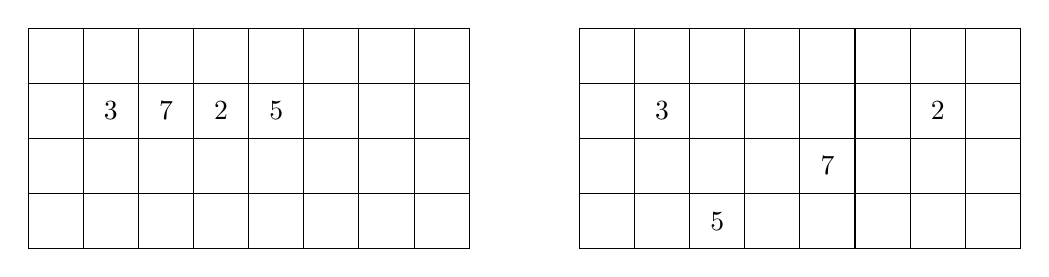
\begin{tikzpicture}[scale=0.7]
\begin{scope}
\draw (0,0) grid (8,4);
\node at (1.5,2.5) {3};
\node at (2.5,2.5) {7};
\node at (3.5,2.5) {2};
\node at (4.5,2.5) {5};
\end{scope}
\begin{scope}[xshift=10cm]
\draw (0,0) grid (8,4);
\node at (1.5,2.5) {3};
\node at (4.5,1.5) {7};
\node at (6.5,2.5) {2};
\node at (2.5,0.5) {5};
\end{scope}
\end{tikzpicture}
\caption{Taulukkolista ja linkitetty lista tietokoneen muistissa.}
\label{fig:taulin}
\end{figure}

Syynä tähän on, että nykyaikaiset tietokoneet
\emph{suosivat} taulukkolistan käyttämistä linkitetyn listan sijaan.
Kuvassa \ref{fig:taulin} näkyy, miten taulukkolista ja linkitetty lista
asettuvat tietokoneen muistissa.
Taulukkolistan alkiot ovat peräkkäin, kun taas linkitetyn
listan alkiot voivat olla eri puolilla muistia sekalaisessa
järjestyksessä.
Nykyaikaisen prosessorin välimuistit ja komentojen ennustus
on toteutettu niin, että ne ovat parhaimmillaan silloin,
kun tieto on tallennettu muistissa peräkkäin -- eli juuri kuten
taulukkolistassa.
Tämä näkyy käytännössä siinä, että taulukkolistan käsittely on selvästi
tehokkaampaa kuin linkitetyn listan käsittely.
\chapter{Algoritmien suunnittelu}

Kuinka voi suunnitella hyvän algoritmin?
On selvää, ettei tähän kysymykseen ole helppoa vastausta.
Yhtä hyvin voisi kysyä, kuinka voi kirjoittaa hyvän romaanin
tai säveltää hyvää musiikkia.

Tällä kurssilla usein esiintyvä tavoitteemme on
saada aikaan tehokas algoritmi, joka toimisi ajassa $O(n)$ tai $O(n \log n)$.
Kun tämä tavoite on tiedossa, voimme ottaa sen algoritmin
suunnittelun lähtökohdaksi ja rajata sen avulla mahdollisia
lähestymistapoja, joita voimme käyttää.

\section{Tehokkaat algoritmit}

Millainen on algoritmi, joka vie aikaa $O(n)$ tai $O(n \log n)$?
Vaadimme algoritmilta,
että kun sille annetaan syötteenä $n$ alkiota,
se saa käyttää jokaisen alkion käsittelyyn
vain pienen määrän aikaa.
Tämä tarkoittaa käytännössä, että algoritmissa saa
esiintyä seuraavan kaltaisia silmukoita:

\begin{code}
for (int i = 0; i < n; i++) {
    // tee jotain nopeaa
}
\end{code}

Tässä ''jotain nopeaa'' tarkoittaa koodia, joka vie aikaa
$O(1)$ tai $O(\log n)$.
Lisäksi koska järjestäminen vie aikaa $O(n \log n)$,
algoritmi voi tarvittaessa järjestää aineistoa.
Kovin paljon muuta tehokas algoritmi ei sitten voikaan tehdä.
Tämä rajoittaa paljon, mitä aineksia voimme laittaa algoritmiin,
mutta voimme ajatella asiaa myös myönteisesti:
vaatimus tehokkuudesta rajaa pois suuren määrän lähestymistapoja,
eli meidän on helpompaa löytää hyvä algoritmi,
kun vaihtoehtojen määrä on pienempi.

Algoritmien suunnittelussa keskeisiä ovat \emph{havainnot}:
haluamme saada käsityksen,
mitä ominaisuuksia ratkaistavaan ongelmaan liittyy,
jotta voimme käyttää niitä algoritmissa.
Voimme tehdä havaintoja tutkimalla ongelman pieniä tapauksia
ja etsimällä riippuvuuksia ja säännöllisyyksiä.
Jos käy hyvin, huomaamme asioita, jotka pätevät kaikissa ongelman
tapauksissa, ja voimme hyödyntää niitä koko tehtävän ratkaisemisessa.

Usein matka kohti tehokasta algoritmia etenee pienin askelin.
Esimerkiksi voimme ensin keksiä algoritmin, joka toimii ajassa $O(2^n)$,
parantaa sitten aikaan $O(n^2)$ ja lopuksi aikaan $O(n \log n)$.
Tässä tapauksessa molemmat askeleet ovat merkittäviä:
ensimmäinen askel muuttaa \emph{eksponentiaalisen} aikavaativuuden
\emph{polynomiseksi} ja toinen askel parantaa vielä aikavaativuutta niin,
että tuloksena on tehokas algoritmi.

\section{Esimerkkejä}

Seuraavaksi käymme läpi joukon esimerkkitehtäviä,
joissa haluamme saada aikaan tehokkaan algoritmin tehtävän ratkaisemiseen,
ja saavutamme tavoitteen tekemällä havaintoja ratkaistavasta ongelmasta.

\subsection{Kolikot}

Meillä on $n$ kolikkoa, joiden arvot ovat $x_1,x_2,\dots,x_n$,
ja haluamme selvittää pienimmän summan, jota \emph{ei} voi muodostaa kolikoista.
Jokaisen kolikon arvo on kokonaisluku väliltä $1 \dots 10^9$.
Esimerkiksi jos kolikot ovat $[1,2,2,9]$, voimme muodostaa summat
$1$, $2$, $1+2=3$, $2+2=4$ ja $1+2+2=5$,
mutta emme voi muodostaa summaa $6$, joten vastaus on $6$.

\subsubsection{Havainto 1}

Tehtävän vastaus on aina muotoa $x+1$, missä $x$ on jokin kolikoista
saatava summa.
Esimerkissä $x=1+2+2=5$.

Voimme siis ratkaista tehtävän
muodostamalla kaikki mahdolliset $n$ kolikon summat
ja etsimällä pienimmän puuttuvan summan.
Algoritmi on kuitenkin hidas, koska $n$ kolikosta voi
muodostaa summan $2^n$ tavalla, ja joudumme käymään läpi kaikki tavat.

\subsubsection{Havainto 2}

Jos haluamme pystyä muodostamaan summan $1$,
meillä on oltava kolikko, jonka arvo on $1$.

Tämä havainto merkitsee sitä, että voimme ratkaista tehtävän
hyvin helposti, jos minkään kolikon arvo ei ole $1$,
koska vastaus on silloin suoraan $0$.
Entä jos jonkin kolikon arvo on $1$?

\subsubsection{Havainto 3}

Jos haluamme pystyä muodostamaan summat $1$ ja $2$,
meillä on oltava kolikko $1$ ja sen lisäksi
toinen kolikko $1$ tai kolikko $2$.

\subsubsection{Havainto 4}

Jos haluamme pystyä muodostamaan summat $1$, $2$ ja $3$,
meillä on oltava kolikot $[1,2]$ tai $[1,1,1]$.

\subsubsection{Havainto 5}


\subsection{X}

\subsection{X}

\chapter{Hajautustaulu}

Ohjelmoinnissa on usein tarvetta
tietorakenteelle, joka pitää yllä alkioiden joukkoa
ja toteuttaa seuraavat operaatiot:

\begin{itemize}
\item lisää alkio $x$ joukkoon
\item tarkista, onko alkio $x$ joukossa
\item poista alkio $x$ joukosta
\end{itemize}

Voimme helposti toteuttaa tällaisen tietorakenteen
tallentamalla joukon alkiot listaan.
Kun lisäämme joukkoon uuden alkion,
lisäämme sen listan loppuun ajassa $O(1)$.
Kun haluamme etsiä alkiota joukosta,
käymme läpi listan, missä kuluu aikaa $O(n)$.
Poistaminen vie myös aikaa $O(n)$, koska meidän täytyy
etsiä poistettava alkio listasta ja poistaa se.
Tämä ei ole tyydyttävä ratkaisu,
koska etsiminen ja poistaminen toimivat hitaasti.

Tässä ja seuraavassa luvussa käymme läpi kaksi
tietorakennetta, joiden avulla voimme toteuttaa kaikki
kolme joukon operaatiota \emph{tehokkaasti}.
Tämän luvun aiheena on hajautustaulu,
jonka avulla pystymme toteuttamaan operaatiot
keskimäärin ajassa $O(1)$.
Seuraavassa luvussa tutustumme binäärihaku\-puuhun,
jonka operaatiot toimivat ajassa $O(\log n)$
ja johon voimme toteuttaa lisäksi alkioiden järjestykseen
liittyviä operaatioita.

\section{Hajautustaulun toiminta}

\emph{Hajautustaulu} on $N$-alkioinen taulukko,
jonka jokaisessa kohdassa on lista joukkoon kuuluvia alkioita.
Jotta voimme käyttää hajautustaulua,
meillä täytyy olla \emph{hajautusfunktio} $f$,
joka antaa \emph{hajautusarvon}
$f(x)$ mille tahansa joukon alkiolle $x$.
Hajautusarvo on kokonaisluku väliltä
$0,1,\dots,N-1$, missä $N$ vastaa hajautustaulun kokoa.
Tallennamme kohdan $k$ listaan ne joukon alkiot,
joiden hajautusarvo on $k$.

\begin{figure}
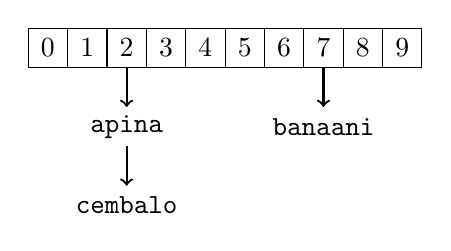
\begin{tikzpicture}[scale=0.5]
\draw (0,0) grid (10,1);
\foreach \x in {0,1,...,9} \node at (0.5+\x,0.5) {\x};
\draw[->,thick] (2.5,0) -- (2.5,-1);
\draw[->,thick] (7.5,0) -- (7.5,-1);
\draw[->,thick] (2.5,-2) -- (2.5,-3);
\node at (2.5,-1.5) {\texttt{apina}};
\node at (7.5,-1.5) {\texttt{banaani}};
\node at (2.5,-3.5) {\texttt{cembalo}};
\end{tikzpicture}
\caption{Hajautustaulu, joka vastaa joukkoa $\{\texttt{apina},\texttt{banaani},\texttt{cembalo}\}$.
Alkioiden \texttt{apina} ja \texttt{cembalo} hajautusarvo on 2,
ja alkion \texttt{banaani} hajautusarvo on 7.}
\label{fig:hajtau}
\end{figure}

Kuvassa \ref{fig:hajtau} on esimerkkinä hajautustaulu,
johon on tallennettu alkiot \texttt{apina}, \texttt{banaani} ja \texttt{cembalo}.
Tässä hajautustaulussa $N=10$, joten kunkin alkion tulee
saada hajautusarvo väliltä $0,1,\dots,9$.
Oletamme, että meillä on käytössämme hajautusfunktio,
joka antaa alkioille \texttt{apina} ja \texttt{cembalo}
hajautusarvon 2 ja alkiolle \texttt{banaani} hajautusarvon 7.
Niinpä alkiot \texttt{apina} ja \texttt{cembalo} ovat
samassa listassa kohdassa 2 ja alkio \texttt{banaani}
on yksin listassa kohdassa 7.
Kaikki muut hajautustaulun listat ovat tällä hetkellä tyhjiä.

Kun haluamme tarkistaa, onko joukossa alkiota $x$,
laskemme ensin sen hajautusarvon $f(x)$.
Tämän jälkeen käymme läpi kaikki kohdan $f(x)$
listassa olevat alkiot ja tarkistamme,
onko jokin niistä alkio $x$.
Vastaavasti kun haluamme lisätä alkion $x$ joukkoon
tai poistaa alkion $x$ joukosta,
teemme muutoksen kohdassa $f(x)$ olevaan listaan.
Näiden operaatioiden aikavaativuus on $O(m)$,
kun jokaisen listan pituus on enintään $m$.

\subsection{Hajautusfunktio}

Hajautusfunktio $f(x)$ määrittää, mihin kohtaan hajautustaulua
alkio $x$ sijoitetaan.
Sen täytyy antaa jokaiselle mahdolliselle alkiolle
hajautusarvo eli kokonaisluku väliltä $0,1,\dots,N-1$,
missä $N$ on hajautustaulun koko.
Lisäksi jotta hajautustaulu olisi käyttökelpoinen,
hajautusfunktion tulisi jakaa alkiot mahdollisimman
\emph{tasaisesti} eri puolille hajautustaulua.
Tällöin hajautustaulun listat ovat lyhyitä ja
operaatiot toimivat tehokkaasti.

\begin{figure}
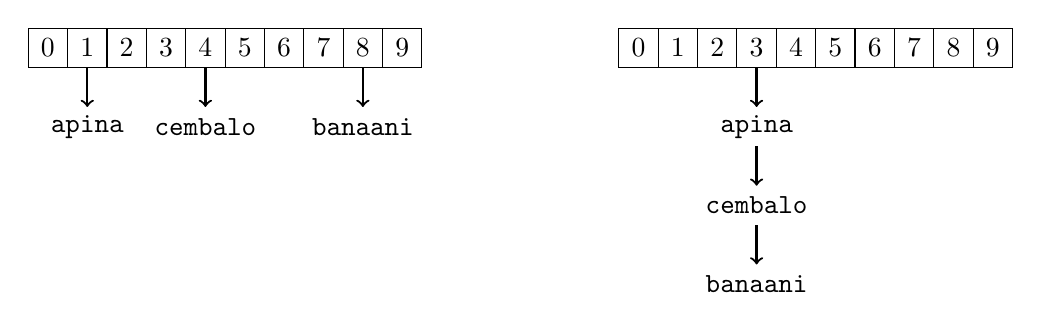
\begin{tikzpicture}[scale=0.5]
\begin{scope}
\draw (0,0) grid (10,1);
\foreach \x in {0,1,...,9} \node at (0.5+\x,0.5) {\x};
\draw[->,thick] (1.5,0) -- (1.5,-1);
\draw[->,thick] (4.5,0) -- (4.5,-1);
\draw[->,thick] (8.5,0) -- (8.5,-1);
\node at (1.5,-1.5) {\texttt{apina}};
\node at (8.5,-1.5) {\texttt{banaani}};
\node at (4.5,-1.5) {\texttt{cembalo}};
\end{scope}
\begin{scope}[xshift=15cm]
\draw (0,0) grid (10,1);
\foreach \x in {0,1,...,9} \node at (0.5+\x,0.5) {\x};
\draw[->,thick] (3.5,0) -- (3.5,-1);
\draw[->,thick] (3.5,-4) -- (3.5,-5);
\draw[->,thick] (3.5,-2) -- (3.5,-3);
\node at (3.5,-1.5) {\texttt{apina}};
\node at (3.5,-5.5) {\texttt{banaani}};
\node at (3.5,-3.5) {\texttt{cembalo}};
\end{scope}
\end{tikzpicture}
\caption{Kaksi hajautustaulua joukolle $\{\texttt{apina},\texttt{banaani},\texttt{cembalo}\}$.
Vasemmassa taulussa hajautus on onnistunut täydellisesti,
oikeassa taulussa kaikki alkiot ovat samassa listassa.}
\label{fig:hajjak}
\end{figure}

Kuva \ref{fig:hajjak} näyttää kaksi hajautustaulua, jotka vastaavat
samaa joukkoa kahdella eri hajautusfunktiolla.
Vasemmassa taulussa hajautus on onnistunut täydellisesti
ja jokainen alkio on omassa listassaan.
Oikeassa taulussa taas kaikki alkiot ovat joutuneet samaan
listaan eikä hajautuksesta ole mitään hyötyä.
Tavoitteemme on, että saisimme aikaan hajautusfunktion,
jonka toiminta on lähempänä vasenta taulua.

Tarkastelemme seuraavaksi esimerkkinä hajautusfunktioita,
joiden avulla voi laskea hajautusarvon merkkijonolle.
Meidän riittää määritellä hajautusfunktio,
joka muuttaa merkkijonon epänegatiiviseksi kokonaisluvuksi,
koska tämän jälkeen saamme helposti kokonaisluvun
väliltä $0 \dots N-1$ ottamalla alkuperäisestä luvusta jakojäännöksen $N$:llä.

Oletamme, että merkkijonossa on $k$ merkkiä,
joiden merkkikoodit\footnote{Käytämme tässä merkkien ASCII-koodeja.
Esimerkiksi Javassa char-merkin \texttt{c} koodin saa
selville kirjoittamalla \texttt{(int)c}, eli esimerkiksi
\texttt{(int)'a'} on 97.} ovat $c_0,c_1,\dots,c_{k-1}$.
Esimerkiksi jos merkkijono on \texttt{apina},
$k=5$ ja koodit ovat $c_0=97$, $c_1=112$, $c_2=105$,
$c_3=110$ ja $c_4=97$.
Seuraavassa on kolme mahdollista tapaa määritellä hajautusfunktio:

\begin{enumerate}
\item Hajautusarvo on merkkijonon pituus $k$.
Esimerkiksi merkkijonon \texttt{apina} hajautusarvo on 5.
\item Hajautusarvo on merkkikoodien summa
\[ c_0 + c_1 + \dots + c_{k-1}.\]
Esimerkiksi merkkijonon \texttt{apina} hajautusarvo on
\[97+112+105+110+97=521.\]
\item Hajautusarvo on summa
\[ A^{k-1} c_0 + A^{k-2} c_1 + \dots + A^0 c_{k-1},\]
missä $A$ on sopiva vakio (\emph{polynominen hajautus}).
Esimerkiksi jos $A=7$, merkkijonon \texttt{apina} hajautusarvo on
\[7^4 \cdot 97+7^3 \cdot 112+7^2 \cdot 105+7^1 \cdot 110+7^0 \cdot 97=61235.\]
\end{enumerate}

Funktiot 1 ja 2 eivät ole käytännössä hyviä hajautusfunktioita,
koska ne antavat saman hajautusarvon monille merkkijonoille.
Funktio 1 antaa kahdelle merkkijonolle saman hajautusarvon,
jos ne ovat yhtä pitkiä,
ja funktio 2 antaa kahdelle merkkijonolle saman hajautusarvon,
jos ne sisältävät samat merkit eri järjestyksessä.

Funktio 3, jota kutsutaan nimellä polynominen hajautus,
on käytännössä hyvä hajautustapa, joka on käytössä esimerkiksi
Javan standardikirjastossa.
Koska hajautusarvo lasketaan painotettuna summana,
kaksi eri merkkijonoa eivät yleensä saa samaa hajautusarvoa.
Toisaalta pystymme laskemaan hajautusarvon tehokkaasti
mille tahansa merkkijonolle.

\subsection{Hajautuksen tehokkuus}

Hajautuksen tehokkuus riippuu kahdesta asiasta:
kuinka suuri hajautustaulu on (parametri $n$)
sekä miten tasaisesti hajautusfunktio jakaa alkiota
eri puolille hajautustaulua.
Jos oletamme, että alkiot jakautuvat tasaisesti
ja joukossa on yhteensä $m$ alkiota,
jokaiseen listaan osuu noin $m/n$ alkiota
eli hajautustaulun operaatiot toimivat $O(m/n)$-ajassa.
Jos edelleen $n$ on valittu niin suureksi,
että $m/n$ on pieni vakio, voimme ajatella,
että hajautustaulun operaatiot toimivat $O(1)$-ajassa.

Tämän analyysin heikkoutena on, että \emph{oletamme}
hajautusfunktion toimivan hyvin ja jakavan alkioita
tasaisesti hajautustauluun. Entä jos näin ei olekaan?
Jos käytämme polynomista hajautusta, miten vakio $A$
pitäisi valita, jotta hajautus onnistuisi hyvin?

Kaikeksi onneksi hajautus toimii yleensä aina käytännössä hyvin.
Riski siitä, että jokainen tai edes suuri osa alkioista
menisi samaan listaan, on niin pieni,
että siitä ei tarvitse murehtia.
Jotkut suosittelevat valitsemaan $A$:n alkuluvuksi,
joka ei ole lähellä 2:n potensseja,
mutta käytännössä muutkaan $A$:n arvot tuskin
tuottavat ongelmia.

Hajautustaulun tehokkuus riippuu kuitenkin aina myös siitä,
mitä alkioita sinne laitetaan.
Vaikka olisimme valinneet hajautustaulun koon ja
hajautusfunktion miten huolellisesti tahansa,
ilkeä vastustaja voi kuitenkin antaa meillä alkioita,
joilla kaikilla on sama hajautusarvo ja jotka
menevät samaan listaan hajautustaulussa.
Tällöin hajautustaulun operaatiot vievät aikaa $O(m)$.
Luvussa 5.2.4 näemme tästä konkreettisen esimerkin.

\section{Hajautus Javassa}

Javassa on kaksi hajautustaulua käyttävää tietorakennetta:
\texttt{HashSet} pitää yllä alkioiden joukkoa
hajautustaulun avulla, ja \texttt{HashMap} säilyttää
joukkoa avain-arvo-pareja, mitä voi ajatella taulukon yleistyksenä.
Seuraavaksi tutustumme tarkemmin näihin rakenteisiin.

\subsection{\texttt{HashSet}-rakenne}

Javan \texttt{HashSet}-rakenne pitää yllä joukkoa alkioista.
Joukkoon voi lisätä alkion metodilla \texttt{add},
ja siitä voi poistaa alkion metodilla \texttt{remove}.
Esimerkiksi seuraava koodi luo joukon, jossa voi olla
kokonaislukuja, ja lisää siihen luvut 3, 5 ja 8.
Tämän jälkeen koodi poistaa luvun 5 joukosta.

\begin{code}
HashSet<Integer> joukko = new HashSet<>();
joukko.add(3);
joukko.add(5);
joukko.add(8);
System.out.println(joukko); // [3, 5, 8]
joukko.remove(5);
System.out.println(joukko); // [3, 8]
\end{code}

Metodin \texttt{contains} avulla voimme selvittää,
esiintyykö tietty alkio joukossa.

\begin{code}
if (joukko.contains(5)) {
    System.out.println("Luku 5 on joukossa");
}
\end{code}

Huomaa, että jokainen alkio voi esiintyä vain kerran joukossa.
Esimerkiksi vaikka seuraava koodi lisää luvun 5 kolmesti
joukkoon, se menee sinne vain ensimmäisellä kerralla ja
muut lisäykset jätetään huomiotta.

\begin{code}
HashSet<Integer> joukko = new HashSet<>();
joukko.add(5);
joukko.add(5);
joukko.add(5);
System.out.println(joukko); // [5]
\end{code}

\subsection{\texttt{HashMap}-rakenne}

\texttt{HashMap}-rakenne pitää yllä joukkoa avain-arvo-pareja.
Rakennetta voi ajatella taulukon yleistyksenä:
$n$ alkion taulukossa avaimet ovat aina kokonaisluvut
$0,1,\ldots,n-1$, mutta \texttt{HashMap} sallii
avaimina minkä tahansa tyyppisiä alkioita eikä niiden
tarvitse olla peräkkäisiä kokonaislukuja.

\texttt{HashMap}-rakenteen määrittelyssä annetaan
kaksi tyyppiä: avaimen ja arvon tyyppi.
Esimerkiksi seuraava koodi luo sanakirjan, jossa sekä
avaimet että arvot ovat merkkijonoja.
Syötämme sanakirjaan merkkijonopareja, jotka kertovat
sanan käännöksen suomesta englanniksi.
Metodi \texttt{put} lisää uuden avain-arvo-parin,
ja metodi \texttt{get} hakee arvon avaimen perusteella.

\begin{code}
HashMap<String,String> sanakirja = new HashMap<>();

sanakirja.put("apina","monkey");
sanakirja.put("banaani","banana");
sanakirja.put("cembalo","harpsichord");

System.out.println(sanakirja.get("banaani")); // banana
\end{code}

Hyödyllinen on myös metodi \texttt{containsKey},
jonka avulla voi tarkastaa, onko tietylle avaimelle
tallennettu arvoa:

\begin{code}
if (sanakirja.containsKey(sana)) {
    System.out.println("Käännös: " + sanakirja.get(sana));
} else {
    System.out.println("Sana puuttuu sanakirjasta!");
}
\end{code}

Koska \texttt{HashMap} on toteutettu hajautustaulun avulla,
sen operaatiot toimivat tehokkaasti keskimäärin $O(1)$-ajassa.

\subsection{Omat luokat}

Javan olioissa on metodi \texttt{hashCode},
jonka avulla olio kertoo pyydettäessä hajautusarvonsa.
Voimme esimerkiksi selvittää merkkijonon \texttt{apina}
hajautusarvon seuraavasti:

\begin{code}
System.out.println("apina".hashCode());
\end{code}

Tämä koodi tulostaa luvun 93022541,
joka on siis merkkijonon \texttt{apina} hajautusarvo Javassa.
On tunnettua, että Java käyttää merkkijonon hajautusarvon laskemiseen
polynomista hajautusta vakiolla $A=31$,
joten voimme laskea Javan hajautusarvon myös itse kaavalla
\[31^4 \cdot 97+31^3 \cdot 112+31^2 \cdot 105+31^1 \cdot 110+31^0 \cdot 97=93022541.\]

Jos haluamme käyttää omia oliota hajautustauluissa,
meidän täytyy toteuttaa luokkaan kaksi metodia:
\texttt{hashCode}, joka antaa olion hajautusarvon,
sekä \texttt{equals},
joka ilmaisee, ovatko kaksi oliota samat.
Jälkimmäinen metodi on tarpeen,
jotta Java pystyy varmistamaan, ovatko saman hajautusarvon
antavat oliot todella samat.


Esimerkiksi jos meillä on luokka \texttt{Piste},
jossa on kenttinä kokonaisluvut \texttt{x} ja \texttt{y},
voisimme toteuttaa metodit seuraavasti:

\begin{code}
class Piste {
    public int x, y;

    public int hashCode() {
        return 97*x+y;
    }
    
    public boolean equals(Object o) {
        Piste p = (Piste)o;
        return x == p.x && y == p.y;
    }
}
\end{code}

Tässä toteutuksessa siis pisteen $(x,y)$ hajautusarvo lasketaan
kaavalla $97x+y$, missä 97 on valitsemamme vakio, jolla ei ole
syvällistä merkitystä.
Nyt kun hajautusfunktio on kunnossa,
voimme luoda vaikkapa \texttt{HashSet}-rakenteen, jossa on pisteitä:

\begin{code}
HashSet<Piste> joukko = new HashSet<Piste>();
\end{code}

\section{Esimerkki: Anagrammit}

Annettuna on lista sanoja ja haluamme jakaa sanat ryhmiin niin,
että kukin ryhmä sisältää sanat, jotka ovat keskenään anagrammeja.
Kaksi sanaa ovat anagrammit, jos ne on mahdollista muuttaa toisikseen
muuttamalla niiden kirjainten järjestystä.

Esimerkiksi jos sanat ovat ''abc'', ''iines'', ''bac'', ''cba'' ja ''sieni'',
niistä muodostuu kaksi ryhmää.
Ensimmäisessä ryhmässä on sanat ''abc'', ''bac'' ja ''cba'',
ja toisessa ryhmässä on sanat ''iines'' ja ''sieni''.

Voimme ratkaista tehtävän tehokkaasti seuraavan havainnon avulla:
jos kaksi sanaa ovat anagrammit ja järjestämme niiden kirjaimet,
niistä tulee samat sanat.
Esimerkiksi sanoissa ''iines'' ja ''sieni'' kirjaimet
järjestettyinä ovat ''eiins''.
Tämän havainnon ansiosta voimme käyttää kunkin anagrammiryhmän
tunnuksena sen sanojen järjestettyä muotoa.

Luomme ryhmiä varten rakenteen

\begin{code}
HashMap<String,ArrayList<String>> ryhmat = new HashMap<>();
\end{code}

jossa avaimena on anagrammiryhmän tunnus ja arvona on lista,
joka sisältää kaikki listaan kuuluvat sanat.
Algoritmin runko näyttää seuraavalta, kun oletamme,
että sanat on tallennettu listaan \texttt{sanat}:

\begin{code}
for (String sana : sanat) {
    String avain = tunnus(sana);
    if (!ryhmat.containsKey(avain)) {
        ryhmat.put(avain,new ArrayList<>());
    }
    ryhmat.get(avain).add(sana);
}
System.out.println(ryhmat);
\end{code}

Tarvitsemme vielä metodin \texttt{tunnus}, joka järjestää
sanan kirjaimet aakkosjärjestykseen.
Jotta voimme järjestää sanan, muutamme sen merkkitaulukoksi,
järjestämme taulukon, ja palautamme sitten uuden merkkijonon,
joka on muodostettu taulukosta.

\begin{code}
String tunnus(String sana) {
    char[] taulu = sana.toCharArray();
    Arrays.sort(taulu);
    return new String(taulu);
}
\end{code}

Esimerkin tapauksessa ohjelmamme tulostus on seuraava:

\begin{code}
{abc=[abc, bac, cba], eiins=[iines, sieni]}
\end{code}

\section{Hajautuksen rikkominen}

\chapter{Keko}

\index{keko}
\index{prioriteettijono}

\emph{Keko} (\emph{heap}) on tietorakenne, jonka operaatiot ovat
alkion lisääminen sekä
pienimmän tai suurimman alkion etsiminen ja poistaminen.
Vaikka voisimme toteuttaa nämä operaatiot myös
binäärihakupuun avulla, keon etuna on, että saamme aikaan
yleistä joukkorakennetta \emph{kevyemmän} rakenteen, kun
rajoitumme tilanteeseen, jossa käytössämme on vain nämä operaatiot.

Tutustumme tässä luvussa binäärikeko-rakenteeseen,
joka on tavallisimmin käytetty kekorakenne.
Binäärikeko toteutetaan binääripuuna,
ja se mahdollistaa alkion etsimisen ajassa $O(1)$ sekä
alkioiden lisäykset ja poistot ajassa $O(\log n)$.
Pystymme toteuttamaan binäärikeon tehokkaasti taulukkona,
koska sen toiminnot ovat yleistä binääripuuta rajatumpia.

\section{Binäärikeko}

\index{binäärikeko}

\emph{Binäärikeko} (\emph{binary heap}) on binääripuu, jonka kaikki tasot
alinta tasoa lukuun ottamatta ovat täynnä solmuja.
Alimman tason solmut on puolestaan sijoitettu
mahdollisimman vasemmalle ylempien solmujen lapsiksi.

\index{minimikeko}
\index{maksimikeko}
\index{kekoehto}

Kun luomme keon, meidän täytyy päättää,
onko se \emph{minimikeko} vai \emph{maksimikeko}.
Minimikeossa voimme etsiä ja poistaa pienimmän alkion,
kun taas maksimikeossa voimme etsiä ja poistaa suurimman alkion.
Keon toiminta perustuu siihen, että jokainen
keon solmu täyttää \emph{kekoehdon}.
Minimikeossa ehtona on, että jokaisen solmun arvo on
pienempi tai yhtä suuri kuin sen kummankin lapsen arvo.
Maksimikeossa puolestaan ehtona on, että jokaisen solmun arvo
on suurempi tai yhtä suuri kuin sen kummankin lapsen arvo.
Kekoehdon ansiosta minimikeon juuressa on keon
pienin alkio ja maksimikeon juuressa on keon suurin alkio.

\begin{figure}
\center
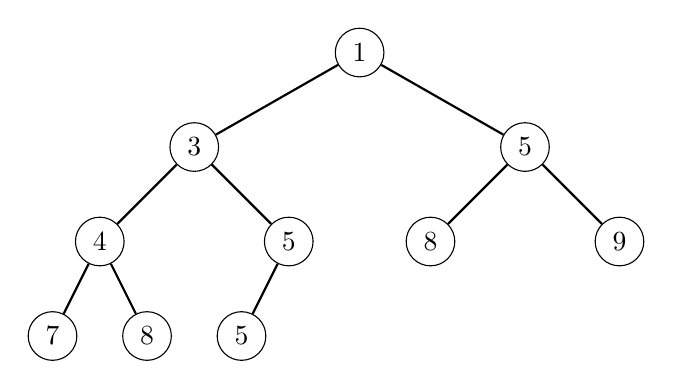
\begin{tikzpicture}[scale=0.6]
\node[draw, circle] (1) at (0,0) {$1$};
\node[draw, circle] (2) at (-3.5,-2) {$3$};
\node[draw, circle] (3) at (3.5,-2) {$5$};
\node[draw, circle] (4) at (-5.5,-4) {$4$};
\node[draw, circle] (5) at (-1.5,-4) {$5$};
\node[draw, circle] (6) at (1.5,-4) {$8$};
\node[draw, circle] (7) at (5.5,-4) {$9$};
\node[draw, circle] (8) at (-6.5,-6) {$7$};
\node[draw, circle] (9) at (-4.5,-6) {$8$};
\node[draw, circle] (10) at (-2.5,-6) {$5$};
\path[draw,thick,-] (1) -- (2);
\path[draw,thick,-] (1) -- (3);
\path[draw,thick,-] (2) -- (4);
\path[draw,thick,-] (2) -- (5);
\path[draw,thick,-] (3) -- (6);
\path[draw,thick,-] (3) -- (7);
\path[draw,thick,-] (4) -- (8);
\path[draw,thick,-] (4) -- (9);
\path[draw,thick,-] (5) -- (10);
\end{tikzpicture}
\caption{Minimikeko, joka sisältää alkiot $[1,3,4,5,5,5,7,8,8,9]$.}
\label{fig:minkek}
\end{figure}

Kuvassa \ref{fig:minkek} on minimikeko,
johon on tallennettu kymmenen alkiota.
Keon kolme ensimmäistä tasoa ovat täynnä
ja neljännellä tasolla kolme ensimmäistä kohtaa on käytetty.
Keon juurena on joukon pienin alkio $1$,
ja kaikki solmut täyttävät kekoehdon.
Huomaa, että sama alkio voi esiintyä monta kertaa keossa,
kuten tässä keossa alkiot $5$ ja $8$.

\subsection{Keon tallentaminen}

Tallennamme binäärikeon \emph{taulukkona},
joka sisältää keon solmujen arvot jär\-jestyksessä
ylhäältä alaspäin ja vasemmalta oikealle.
Tämä tehokas tallennustapa on mahdollinen,
koska keon kaikki tasot ovat täynnä solmuja.
Tavallinen tapa on tallentaa keko taulukkoon niin,
että indeksointi alkaa 1:stä.
Esimerkiksi kuvan \ref{fig:minkek} keko vastaa seuraavaa taulukkoa:
\vspace{5px}

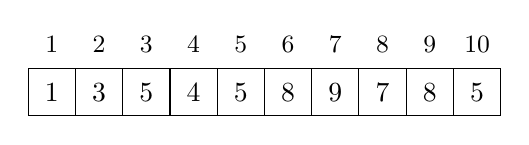
\begin{tikzpicture}[scale=0.6]
\draw (0,0) grid (10,1);
\foreach \x in {1,...,10} \node at (-0.5+\x,1.5) {\small \x};
\foreach \x/\v in {1/1,2/3,3/5,4/4,5/5,6/8,7/9,8/7,9/8,10/5} \node at (-0.5+\x,0.5) {\v};
\end{tikzpicture}

\vspace{5px}
Taulukkototeutuksen etuna on, että voimme laskea
helposti, missä kohdissa keon alkiot ovat taulukossa.
Ensinnäkin keon juuri eli pienin tai suurin alkio
on aina kohdassa $1$.
Lisäksi jos tiedämme, että tietty solmu on kohdassa $k$,
niin solmun vasen lapsi on kohdassa $2k$,
solmun oikea lapsi on kohdassa $2k+1$ ja
solmun vanhempi on kohdassa $\lfloor k/2 \rfloor$.
Esimerkissämme solmu $3$
on taulukossa kohdassa $2$,
joten sen vasen lapsi on kohdassa $4$,
oikea lapsi on kohdassa $5$ ja
vanhempi on kohdassa $1$.

Käytännössä haluamme yleensä,
että pystymme lisäämään kekoon uusia alkioita,
jolloin saattaa olla tarpeen suurentaa taulukkoa.
Voimme toteuttaa tämän samalla tavalla kuin taulukkolistassa,
jolloin taulukon suurentaminen ei hidasta keon operaatioita.

\subsection{Operaatioiden toteutus}

On helppoa etsiä minimikeon pienin alkio
tai maksimikeon suurin alkio $O(1)$-ajassa,
koska tämä alkio on aina keon juuressa.
Seuraavaksi näemme, kuinka voimme toteuttaa alkion lisäämisen
sekä pienimmän tai suurimman alkion poistamisen $O(\log n)$-ajassa.

\subsubsection{Alkion lisääminen}

Kun lisäämme uuden alkion kekoon, lisäämme sen ensin seuraavaan
vapaana olevaan paikkaan puussa. Jos alimmalla tasolla on tilaa,
lisäämme sen sinne mahdollisimman vasemmalle,
ja muuten aloitamme uuden tason, jossa on toistaiseksi vain lisättävä solmu.
Alkion lisäämisen jälkeen meidän täytyy varmistaa,
että kekoehto säilyy edelleen voimassa.
Tämä tapahtuu siirtämällä alkiota ylöspäin keossa,
kunnes kekoehto tulee voimaan.

\begin{figure}
\center
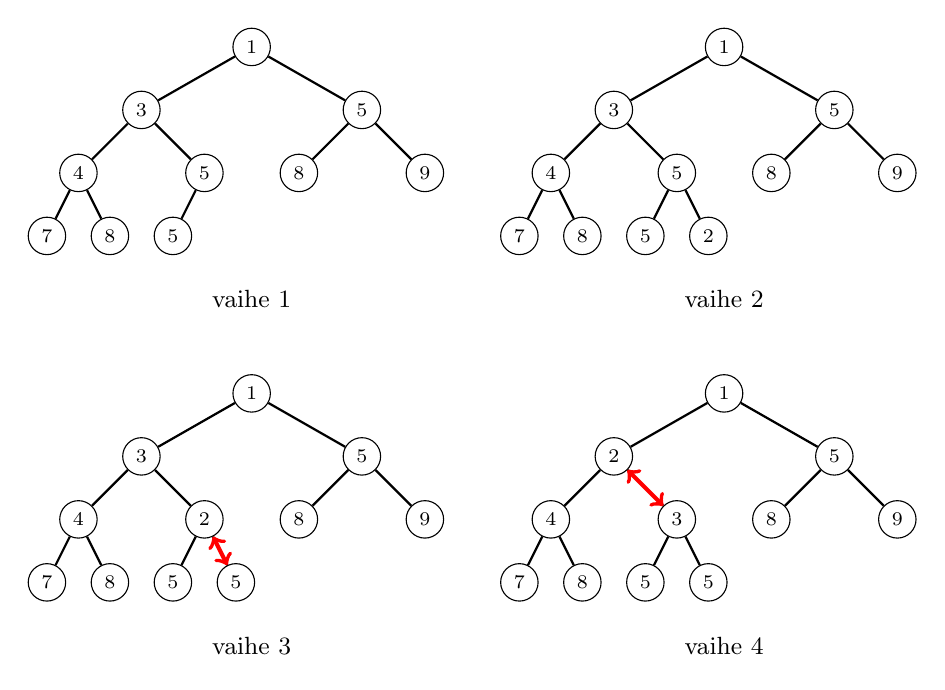
\begin{tikzpicture}[scale=0.4]
\scriptsize
\begin{scope}
\node[draw, circle] (1) at (0,0) {$1$};
\node[draw, circle] (2) at (-3.5,-2) {$3$};
\node[draw, circle] (3) at (3.5,-2) {$5$};
\node[draw, circle] (4) at (-5.5,-4) {$4$};
\node[draw, circle] (5) at (-1.5,-4) {$5$};
\node[draw, circle] (6) at (1.5,-4) {$8$};
\node[draw, circle] (7) at (5.5,-4) {$9$};
\node[draw, circle] (8) at (-6.5,-6) {$7$};
\node[draw, circle] (9) at (-4.5,-6) {$8$};
\node[draw, circle] (10) at (-2.5,-6) {$5$};
\path[draw,thick,-] (1) -- (2);
\path[draw,thick,-] (1) -- (3);
\path[draw,thick,-] (2) -- (4);
\path[draw,thick,-] (2) -- (5);
\path[draw,thick,-] (3) -- (6);
\path[draw,thick,-] (3) -- (7);
\path[draw,thick,-] (4) -- (8);
\path[draw,thick,-] (4) -- (9);
\path[draw,thick,-] (5) -- (10);
\node at (0,-8) {\small vaihe $1$};
\end{scope}
\begin{scope}[xshift=15cm]
\node[draw, circle] (1) at (0,0) {$1$};
\node[draw, circle] (2) at (-3.5,-2) {$3$};
\node[draw, circle] (3) at (3.5,-2) {$5$};
\node[draw, circle] (4) at (-5.5,-4) {$4$};
\node[draw, circle] (5) at (-1.5,-4) {$5$};
\node[draw, circle] (6) at (1.5,-4) {$8$};
\node[draw, circle] (7) at (5.5,-4) {$9$};
\node[draw, circle] (8) at (-6.5,-6) {$7$};
\node[draw, circle] (9) at (-4.5,-6) {$8$};
\node[draw, circle] (10) at (-2.5,-6) {$5$};
\node[draw, circle] (11) at (-0.5,-6) {$2$};
\path[draw,thick,-] (1) -- (2);
\path[draw,thick,-] (1) -- (3);
\path[draw,thick,-] (2) -- (4);
\path[draw,thick,-] (2) -- (5);
\path[draw,thick,-] (3) -- (6);
\path[draw,thick,-] (3) -- (7);
\path[draw,thick,-] (4) -- (8);
\path[draw,thick,-] (4) -- (9);
\path[draw,thick,-] (5) -- (10);
\path[draw,thick,-] (5) -- (11);
\node at (0,-8) {\small vaihe $2$};
\end{scope}
\begin{scope}[yshift=-11cm]
\node[draw, circle] (1) at (0,0) {$1$};
\node[draw, circle] (2) at (-3.5,-2) {$3$};
\node[draw, circle] (3) at (3.5,-2) {$5$};
\node[draw, circle] (4) at (-5.5,-4) {$4$};
\node[draw, circle] (5) at (-1.5,-4) {$2$};
\node[draw, circle] (6) at (1.5,-4) {$8$};
\node[draw, circle] (7) at (5.5,-4) {$9$};
\node[draw, circle] (8) at (-6.5,-6) {$7$};
\node[draw, circle] (9) at (-4.5,-6) {$8$};
\node[draw, circle] (10) at (-2.5,-6) {$5$};
\node[draw, circle] (11) at (-0.5,-6) {$5$};
\path[draw,thick,-] (1) -- (2);
\path[draw,thick,-] (1) -- (3);
\path[draw,thick,-] (2) -- (4);
\path[draw,thick,-] (2) -- (5);
\path[draw,thick,-] (3) -- (6);
\path[draw,thick,-] (3) -- (7);
\path[draw,thick,-] (4) -- (8);
\path[draw,thick,-] (4) -- (9);
\path[draw,thick,-] (5) -- (10);
\path[draw,thick,-] (5) -- (11);
\node at (0,-8) {\small vaihe $3$};
\path[draw,thick,<->,red,line width=1.5pt] (5) -- (11);
\end{scope}
\begin{scope}[yshift=-11cm,xshift=15cm]
\node[draw, circle] (1) at (0,0) {$1$};
\node[draw, circle] (2) at (-3.5,-2) {$2$};
\node[draw, circle] (3) at (3.5,-2) {$5$};
\node[draw, circle] (4) at (-5.5,-4) {$4$};
\node[draw, circle] (5) at (-1.5,-4) {$3$};
\node[draw, circle] (6) at (1.5,-4) {$8$};
\node[draw, circle] (7) at (5.5,-4) {$9$};
\node[draw, circle] (8) at (-6.5,-6) {$7$};
\node[draw, circle] (9) at (-4.5,-6) {$8$};
\node[draw, circle] (10) at (-2.5,-6) {$5$};
\node[draw, circle] (11) at (-0.5,-6) {$5$};
\path[draw,thick,-] (1) -- (2);
\path[draw,thick,-] (1) -- (3);
\path[draw,thick,-] (2) -- (4);
\path[draw,thick,-] (2) -- (5);
\path[draw,thick,-] (3) -- (6);
\path[draw,thick,-] (3) -- (7);
\path[draw,thick,-] (4) -- (8);
\path[draw,thick,-] (4) -- (9);
\path[draw,thick,-] (5) -- (10);
\path[draw,thick,-] (5) -- (11);
\node at (0,-8) {\small vaihe $4$};
\path[draw,thick,<->,red,line width=1.5pt] (2) -- (5);
\end{scope}
\end{tikzpicture}
\caption{Lisäämme alkion 2 kekoon ja nostamme sitä ylöspäin,
kunnes kekoehto tulee jälleen voimaan.}
\label{fig:keklis}
\end{figure}

Kuva \ref{fig:keklis} näyttää, mitä tapahtuu, kun lisäämme
alkion  $2$ esimerkkikekoomme.
Lisäämme alkion ensimmäiseen vapaaseen kohtaan
keon alimmalla tasolla.
Koska alkio 2 on pienempi kuin sen vanhempi 5,
vaihdamme nämä alkiot keskenään.
Tämän jälkeen alkio 2 on pienempi kuin sen vanhempi 3,
joten vaihdamme myös nämä alkiot keskenään.
Nyt kekoehto on voimassa eikä meidän tarvitse enää
tehdä muutoksia kekoon.

Alkion lisääminen kekoon vie aikaa $O(\log n)$,
koska keossa on $O(\log n)$ tasoa ja kuljemme aina
ylöspäin keon pohjalta huippua kohden,
kunnes olemme löytäneet alkiolle sopivan paikan keosta.

\subsubsection{Alkion poistaminen}

Kun haluamme poistaa keon juuressa olevan alkion,
siirrämme ensin keon viimeisen alkion keon juureksi
ja poistamme sille kuuluneen solmun.
Tämän jälkeen lasketamme juureen nostettua alkiota
alaspäin keossa, kunnes kekoehto on jälleen voimassa kaikkialla.
Koska solmulla voi olla kaksi lasta,
voi olla kaksi vaihtoehtoa,
kumman lapsista nostamme ylemmäs.
Jos keko on minimikeko, valitsemme lapsen,
jossa on pienempi arvo,
ja jos keko on maksimikeko, valitsemme vastaavasti
lapsen, jossa on suurempi arvo.

\begin{figure}
\center
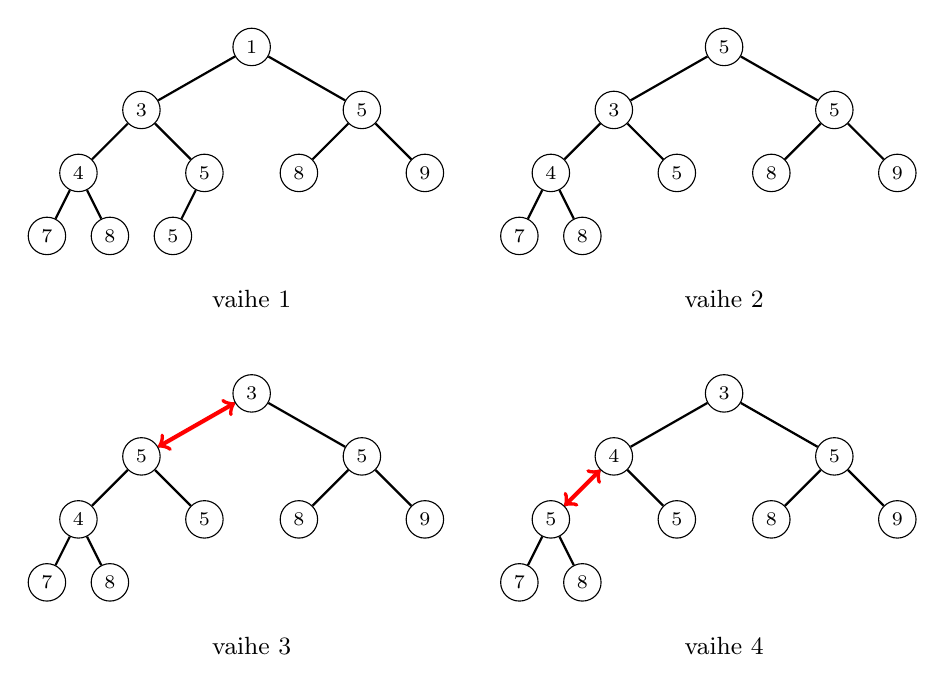
\begin{tikzpicture}[scale=0.4]
\scriptsize
\begin{scope}
\node[draw, circle] (1) at (0,0) {$1$};
\node[draw, circle] (2) at (-3.5,-2) {$3$};
\node[draw, circle] (3) at (3.5,-2) {$5$};
\node[draw, circle] (4) at (-5.5,-4) {$4$};
\node[draw, circle] (5) at (-1.5,-4) {$5$};
\node[draw, circle] (6) at (1.5,-4) {$8$};
\node[draw, circle] (7) at (5.5,-4) {$9$};
\node[draw, circle] (8) at (-6.5,-6) {$7$};
\node[draw, circle] (9) at (-4.5,-6) {$8$};
\node[draw, circle] (10) at (-2.5,-6) {$5$};
\path[draw,thick,-] (1) -- (2);
\path[draw,thick,-] (1) -- (3);
\path[draw,thick,-] (2) -- (4);
\path[draw,thick,-] (2) -- (5);
\path[draw,thick,-] (3) -- (6);
\path[draw,thick,-] (3) -- (7);
\path[draw,thick,-] (4) -- (8);
\path[draw,thick,-] (4) -- (9);
\path[draw,thick,-] (5) -- (10);
\node at (0,-8) {\small vaihe $1$};
\end{scope}
\begin{scope}[xshift=15cm]
\node[draw, circle] (1) at (0,0) {$5$};
\node[draw, circle] (2) at (-3.5,-2) {$3$};
\node[draw, circle] (3) at (3.5,-2) {$5$};
\node[draw, circle] (4) at (-5.5,-4) {$4$};
\node[draw, circle] (5) at (-1.5,-4) {$5$};
\node[draw, circle] (6) at (1.5,-4) {$8$};
\node[draw, circle] (7) at (5.5,-4) {$9$};
\node[draw, circle] (8) at (-6.5,-6) {$7$};
\node[draw, circle] (9) at (-4.5,-6) {$8$};
\path[draw,thick,-] (1) -- (2);
\path[draw,thick,-] (1) -- (3);
\path[draw,thick,-] (2) -- (4);
\path[draw,thick,-] (2) -- (5);
\path[draw,thick,-] (3) -- (6);
\path[draw,thick,-] (3) -- (7);
\path[draw,thick,-] (4) -- (8);
\path[draw,thick,-] (4) -- (9);
\node at (0,-8) {\small vaihe $2$};
\end{scope}
\begin{scope}[yshift=-11cm]
\node[draw, circle] (1) at (0,0) {$3$};
\node[draw, circle] (2) at (-3.5,-2) {$5$};
\node[draw, circle] (3) at (3.5,-2) {$5$};
\node[draw, circle] (4) at (-5.5,-4) {$4$};
\node[draw, circle] (5) at (-1.5,-4) {$5$};
\node[draw, circle] (6) at (1.5,-4) {$8$};
\node[draw, circle] (7) at (5.5,-4) {$9$};
\node[draw, circle] (8) at (-6.5,-6) {$7$};
\node[draw, circle] (9) at (-4.5,-6) {$8$};
\path[draw,thick,-] (1) -- (2);
\path[draw,thick,-] (1) -- (3);
\path[draw,thick,-] (2) -- (4);
\path[draw,thick,-] (2) -- (5);
\path[draw,thick,-] (3) -- (6);
\path[draw,thick,-] (3) -- (7);
\path[draw,thick,-] (4) -- (8);
\path[draw,thick,-] (4) -- (9);
\node at (0,-8) {\small vaihe $3$};
\path[draw,thick,<->,red,line width=1.5pt] (1) -- (2);
\end{scope}
\begin{scope}[yshift=-11cm,xshift=15cm]
\node[draw, circle] (1) at (0,0) {$3$};
\node[draw, circle] (2) at (-3.5,-2) {$4$};
\node[draw, circle] (3) at (3.5,-2) {$5$};
\node[draw, circle] (4) at (-5.5,-4) {$5$};
\node[draw, circle] (5) at (-1.5,-4) {$5$};
\node[draw, circle] (6) at (1.5,-4) {$8$};
\node[draw, circle] (7) at (5.5,-4) {$9$};
\node[draw, circle] (8) at (-6.5,-6) {$7$};
\node[draw, circle] (9) at (-4.5,-6) {$8$};
\path[draw,thick,-] (1) -- (2);
\path[draw,thick,-] (1) -- (3);
\path[draw,thick,-] (2) -- (4);
\path[draw,thick,-] (2) -- (5);
\path[draw,thick,-] (3) -- (6);
\path[draw,thick,-] (3) -- (7);
\path[draw,thick,-] (4) -- (8);
\path[draw,thick,-] (4) -- (9);
\node at (0,-8) {\small vaihe $4$};
\path[draw,thick,<->,red,line width=1.5pt] (2) -- (4);
\end{scope}
\end{tikzpicture}
\caption{Poistamme keon juuressa olevan alkion korvaamalla sen viimeisellä alkiolla
ja laskettamalla sitä alaspäin puussa.}
\label{fig:kekpoi}
\end{figure}

Kuva \ref{fig:kekpoi} näyttää, kuinka poistamme
esimerkkikeostamme pienimmän alkion eli juuressa
olevan alkion 1.
Aluksi korvaamme alkion 1
keon viimeisellä alkiolla 5 ja poistamme keosta
alkiolle 5 kuuluneen solmun.
Tämän jälkeen vaihdamme keskenään alkion 5
ja sen vasemman lapsen alkion 3,
ja sitten vielä alkion 5 ja sen vasemman lapsen alkion 4.
Tämän jälkeen kekoehto on voimassa ja olemme onnistuneet
poistamaan pienimmän alkion keosta.

Alkion poistaminen keosta vie aikaa $O(\log n)$,
koska keossa on $O(\log n)$ tasoa ja kuljemme polkua
alaspäin keon huipulta pohjaa kohden.

\section{Lisää keosta}

Koska keko on tallennettu taulukkona,
voimme tulkita minkä tahansa taulukon kekona,
kunhan vain kekoehto on voimassa taulukon kaikissa kohdissa.
Käymme seuraavaksi läpi menetelmän, jonka avulla voimme
\emph{muuttaa} taulukon keoksi $O(n)$-ajassa.
Tämän jälkeen tutustumme kekojärjestämiseen,
joka on $O(n \log n)$-aikainen järjestämisalgoritmi.

\subsection{Taulukosta keoksi}

Oletetaan, että meillä on $n$ alkiota sisältävä taulukko
ja haluamme muuttaa sen keoksi.
Suoraviivainen tapa on luoda tyhjä keko ja
lisätä jokainen taulukon alkio siihen erikseen $O(\log n)$-ajassa.
Tällä tavalla saamme rakennettua keon $O(n \log n)$-ajassa.
Osoittautuu kuitenkin, että pystymme myös muuttamaan taulukon
\emph{suoraan} keoksi tehokkaammin ajassa $O(n)$.

Ideana on järjestää alkuperäisen taulukon alkioita uudestaan niin,
että kekoehto tulee voimaan taulukon jokaiseen kohtaan --
jolloin taulukko on muuttunut keoksi.
Käymme läpi taulukon alkiot lopusta alkuun ja varmistamme
jokaisessa kohdassa, että kekoehto on voimassa kyseisestä
kohdasta alkavassa alipuussa.
Jos kekoehto ei ole voimassa, korjaamme sen laskettamalla
kyseisen kohdan alkiota alaspäin keossa.
Kun lopulta pääsemme taulukon alkuun, kekoehto on voimassa
koko taulukossa.

\begin{figure}
\center
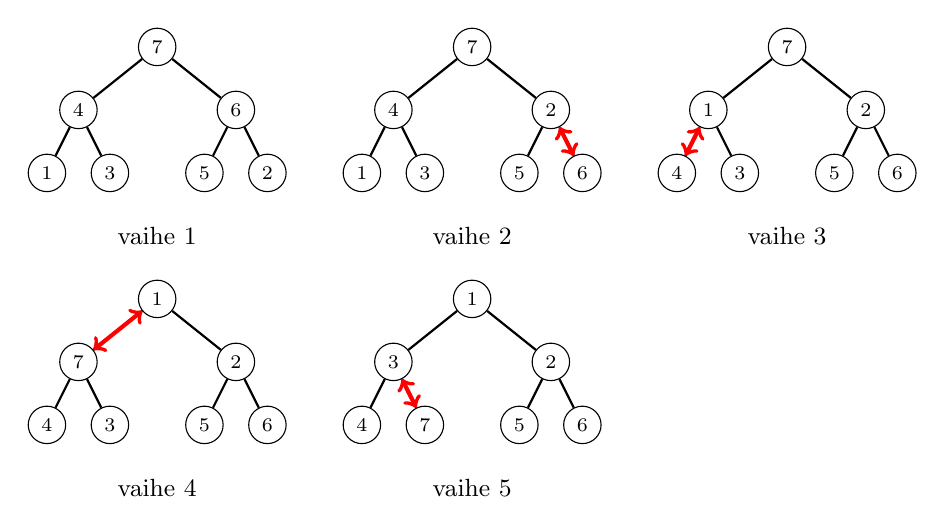
\begin{tikzpicture}[scale=0.4]
\scriptsize
\begin{scope}
\node[draw, circle] (1) at (0,0) {$7$};
\node[draw, circle] (2) at (-2.5,-2) {$4$};
\node[draw, circle] (3) at (2.5,-2) {$6$};
\node[draw, circle] (4) at (-3.5,-4) {$1$};
\node[draw, circle] (5) at (-1.5,-4) {$3$};
\node[draw, circle] (6) at (1.5,-4) {$5$};
\node[draw, circle] (7) at (3.5,-4) {$2$};
\path[draw,thick,-] (1) -- (2);
\path[draw,thick,-] (1) -- (3);
\path[draw,thick,-] (2) -- (4);
\path[draw,thick,-] (2) -- (5);
\path[draw,thick,-] (3) -- (6);
\path[draw,thick,-] (3) -- (7);
\node at (0,-6) {\small vaihe $1$};
\end{scope}
\begin{scope}[xshift=10cm]
\node[draw, circle] (1) at (0,0) {$7$};
\node[draw, circle] (2) at (-2.5,-2) {$4$};
\node[draw, circle] (3) at (2.5,-2) {$2$};
\node[draw, circle] (4) at (-3.5,-4) {$1$};
\node[draw, circle] (5) at (-1.5,-4) {$3$};
\node[draw, circle] (6) at (1.5,-4) {$5$};
\node[draw, circle] (7) at (3.5,-4) {$6$};
\path[draw,thick,-] (1) -- (2);
\path[draw,thick,-] (1) -- (3);
\path[draw,thick,-] (2) -- (4);
\path[draw,thick,-] (2) -- (5);
\path[draw,thick,-] (3) -- (6);
\path[draw,thick,-] (3) -- (7);
\node at (0,-6) {\small vaihe $2$};
\path[draw,thick,<->,red,line width=1.5pt] (3) -- (7);
\end{scope}
\begin{scope}[xshift=20cm]
\node[draw, circle] (1) at (0,0) {$7$};
\node[draw, circle] (2) at (-2.5,-2) {$1$};
\node[draw, circle] (3) at (2.5,-2) {$2$};
\node[draw, circle] (4) at (-3.5,-4) {$4$};
\node[draw, circle] (5) at (-1.5,-4) {$3$};
\node[draw, circle] (6) at (1.5,-4) {$5$};
\node[draw, circle] (7) at (3.5,-4) {$6$};
\path[draw,thick,-] (1) -- (2);
\path[draw,thick,-] (1) -- (3);
\path[draw,thick,-] (2) -- (4);
\path[draw,thick,-] (2) -- (5);
\path[draw,thick,-] (3) -- (6);
\path[draw,thick,-] (3) -- (7);
\node at (0,-6) {\small vaihe $3$};
\path[draw,thick,<->,red,line width=1.5pt] (2) -- (4);
\end{scope}
\begin{scope}[yshift=-8cm]
\node[draw, circle] (1) at (0,0) {$1$};
\node[draw, circle] (2) at (-2.5,-2) {$7$};
\node[draw, circle] (3) at (2.5,-2) {$2$};
\node[draw, circle] (4) at (-3.5,-4) {$4$};
\node[draw, circle] (5) at (-1.5,-4) {$3$};
\node[draw, circle] (6) at (1.5,-4) {$5$};
\node[draw, circle] (7) at (3.5,-4) {$6$};
\path[draw,thick,-] (1) -- (2);
\path[draw,thick,-] (1) -- (3);
\path[draw,thick,-] (2) -- (4);
\path[draw,thick,-] (2) -- (5);
\path[draw,thick,-] (3) -- (6);
\path[draw,thick,-] (3) -- (7);
\node at (0,-6) {\small vaihe $4$};
\path[draw,thick,<->,red,line width=1.5pt] (1) -- (2);
\end{scope}
\begin{scope}[yshift=-8cm,xshift=10cm]
\node[draw, circle] (1) at (0,0) {$1$};
\node[draw, circle] (2) at (-2.5,-2) {$3$};
\node[draw, circle] (3) at (2.5,-2) {$2$};
\node[draw, circle] (4) at (-3.5,-4) {$4$};
\node[draw, circle] (5) at (-1.5,-4) {$7$};
\node[draw, circle] (6) at (1.5,-4) {$5$};
\node[draw, circle] (7) at (3.5,-4) {$6$};
\path[draw,thick,-] (1) -- (2);
\path[draw,thick,-] (1) -- (3);
\path[draw,thick,-] (2) -- (4);
\path[draw,thick,-] (2) -- (5);
\path[draw,thick,-] (3) -- (6);
\path[draw,thick,-] (3) -- (7);
\node at (0,-6) {\small vaihe $5$};
\path[draw,thick,<->,red,line width=1.5pt] (2) -- (5);
\end{scope}
\end{tikzpicture}
\caption{Muutamme taulukon keoksi korjaamalla kekoehdon alipuissa.}
\label{fig:taukek}
\end{figure}

Kuva \ref{fig:taukek} näyttää esimerkin, jossa muutamme taulukon
$[7,4,6,1,3,5,2]$ minimikeoksi.
Kun tulkitsemme taulukon kekona, kekoehto on aluksi
rikki monessa taulukon kohdassa.
Ensin korjaamme kekoehdon tason 2 alipuissa vaihtamalla
keskenään alkiot 2 ja 6 ja sitten alkiot 1 ja 4.
Tämän jälkeen korjaamme kekoehdon tason 1 alipuussa
eli koko keossa laskettamalla alkion 7 keon huipulta pohjalle.
Nyt kekoehto on voimassa kaikkialla taulukossa,
joten olemme onnistuneet muuttamaan taulukon keoksi.

Miksi sitten tämä vie aikaa vain $O(n)$?
Oletetaan, että keossa on $h$ tasoa ja kaikki
tasot ovat täynnä solmuja, eli keossa on $n=2^h-1$ solmua.
Laskemme jokaiselle tasolle, montako alkiota laskeutuu
enintään jostakin tämän tason solmusta alaspäin.
Ensinnäkin tasolta 1 tasolle 2 laskeutuu enintään 1 alkio --
juuressa oleva alkio.
Vastaavasti
tasolta 2 tasolle 3 laskeutuu enintään $1+2$ alkiota
ja
tasolta 3 tasolle 4 laskeutuu enintään $1+2+4$ alkiota.
Yleisemmin tasolta $k$ tasolle $k+1$ laskeutuu
enintään $1+2+\dots+2^{k-1} = 2^k-1$ alkiota
Koska tasoja on $h$ ja alimmalta tasolta ei voi laskeutua alaspäin,
kokonaistyömäärä on enintään
\[(2^1-1)+(2^2-1)+\dots+(2^{h-1}-1)=2^h-h \le n,\]
joten aikaa kuluu vain $O(n)$.

\subsection{Kekojärjestäminen}

\index{kekojärjestäminen}

\emph{Kekojärjestäminen} (\emph{heap sort}) on järjestämisalgoritmi,
jonka toiminta perustuu kekoon.
Ideana on muuttaa järjestettävä taulukko ensin keoksi
ja sen jälkeen poistaa alkiot keosta yksi kerrallaan
järjestyksessä.
Kekojärjestäminen vie aikaa $O(n \log n)$,
koska taulukon muuttaminen keoksi vie aikaa $O(n)$
ja $n$ alkion poistaminen keosta vie aikaa $O(n \log n)$.

\begin{figure}
\center
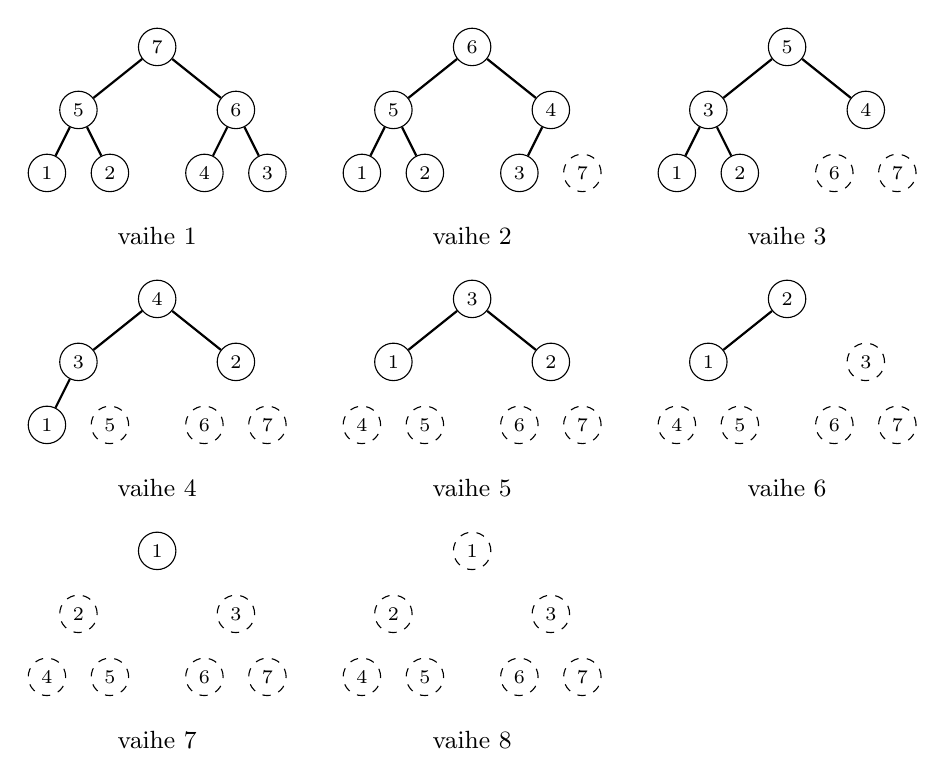
\begin{tikzpicture}[scale=0.4]
\scriptsize
\begin{scope}
\node[draw, circle] (1) at (0,0) {$7$};
\node[draw, circle] (2) at (-2.5,-2) {$5$};
\node[draw, circle] (3) at (2.5,-2) {$6$};
\node[draw, circle] (4) at (-3.5,-4) {$1$};
\node[draw, circle] (5) at (-1.5,-4) {$2$};
\node[draw, circle] (6) at (1.5,-4) {$4$};
\node[draw, circle] (7) at (3.5,-4) {$3$};
\path[draw,thick,-] (1) -- (2);
\path[draw,thick,-] (1) -- (3);
\path[draw,thick,-] (2) -- (4);
\path[draw,thick,-] (2) -- (5);
\path[draw,thick,-] (3) -- (6);
\path[draw,thick,-] (3) -- (7);
\node at (0,-6) {\small vaihe $1$};
\end{scope}
\begin{scope}[xshift=10cm]
\node[draw, circle] (1) at (0,0) {$6$};
\node[draw, circle] (2) at (-2.5,-2) {$5$};
\node[draw, circle] (3) at (2.5,-2) {$4$};
\node[draw, circle] (4) at (-3.5,-4) {$1$};
\node[draw, circle] (5) at (-1.5,-4) {$2$};
\node[draw, circle] (6) at (1.5,-4) {$3$};
\node[draw, circle, dashed] (7) at (3.5,-4) {$7$};
\path[draw,thick,-] (1) -- (2);
\path[draw,thick,-] (1) -- (3);
\path[draw,thick,-] (2) -- (4);
\path[draw,thick,-] (2) -- (5);
\path[draw,thick,-] (3) -- (6);
\node at (0,-6) {\small vaihe $2$};
\end{scope}
\begin{scope}[xshift=20cm]
\node[draw, circle] (1) at (0,0) {$5$};
\node[draw, circle] (2) at (-2.5,-2) {$3$};
\node[draw, circle] (3) at (2.5,-2) {$4$};
\node[draw, circle] (4) at (-3.5,-4) {$1$};
\node[draw, circle] (5) at (-1.5,-4) {$2$};
\node[draw, circle, dashed] (6) at (1.5,-4) {$6$};
\node[draw, circle, dashed] (7) at (3.5,-4) {$7$};
\path[draw,thick,-] (1) -- (2);
\path[draw,thick,-] (1) -- (3);
\path[draw,thick,-] (2) -- (4);
\path[draw,thick,-] (2) -- (5);
\node at (0,-6) {\small vaihe $3$};
\end{scope}
\begin{scope}[xshift=0cm,yshift=-8cm]
\node[draw, circle] (1) at (0,0) {$4$};
\node[draw, circle] (2) at (-2.5,-2) {$3$};
\node[draw, circle] (3) at (2.5,-2) {$2$};
\node[draw, circle] (4) at (-3.5,-4) {$1$};
\node[draw, circle, dashed] (5) at (-1.5,-4) {$5$};
\node[draw, circle, dashed] (6) at (1.5,-4) {$6$};
\node[draw, circle, dashed] (7) at (3.5,-4) {$7$};
\path[draw,thick,-] (1) -- (2);
\path[draw,thick,-] (1) -- (3);
\path[draw,thick,-] (2) -- (4);
\node at (0,-6) {\small vaihe $4$};
\end{scope}
\begin{scope}[xshift=10cm,yshift=-8cm]
\node[draw, circle] (1) at (0,0) {$3$};
\node[draw, circle] (2) at (-2.5,-2) {$1$};
\node[draw, circle] (3) at (2.5,-2) {$2$};
\node[draw, circle, dashed] (4) at (-3.5,-4) {$4$};
\node[draw, circle, dashed] (5) at (-1.5,-4) {$5$};
\node[draw, circle, dashed] (6) at (1.5,-4) {$6$};
\node[draw, circle, dashed] (7) at (3.5,-4) {$7$};
\path[draw,thick,-] (1) -- (2);
\path[draw,thick,-] (1) -- (3);
\node at (0,-6) {\small vaihe $5$};
\end{scope}
\begin{scope}[xshift=20cm,yshift=-8cm]
\node[draw, circle] (1) at (0,0) {$2$};
\node[draw, circle] (2) at (-2.5,-2) {$1$};
\node[draw, circle, dashed] (3) at (2.5,-2) {$3$};
\node[draw, circle, dashed] (4) at (-3.5,-4) {$4$};
\node[draw, circle, dashed] (5) at (-1.5,-4) {$5$};
\node[draw, circle, dashed] (6) at (1.5,-4) {$6$};
\node[draw, circle, dashed] (7) at (3.5,-4) {$7$};
\path[draw,thick,-] (1) -- (2);
\node at (0,-6) {\small vaihe $6$};
\end{scope}
\begin{scope}[xshift=0cm,yshift=-16cm]
\node[draw, circle] (1) at (0,0) {$1$};
\node[draw, circle, dashed] (2) at (-2.5,-2) {$2$};
\node[draw, circle, dashed] (3) at (2.5,-2) {$3$};
\node[draw, circle, dashed] (4) at (-3.5,-4) {$4$};
\node[draw, circle, dashed] (5) at (-1.5,-4) {$5$};
\node[draw, circle, dashed] (6) at (1.5,-4) {$6$};
\node[draw, circle, dashed] (7) at (3.5,-4) {$7$};
\node at (0,-6) {\small vaihe $7$};
\end{scope}
\begin{scope}[xshift=10cm,yshift=-16cm]
\node[draw, circle, dashed] (1) at (0,0) {$1$};
\node[draw, circle, dashed] (2) at (-2.5,-2) {$2$};
\node[draw, circle, dashed] (3) at (2.5,-2) {$3$};
\node[draw, circle, dashed] (4) at (-3.5,-4) {$4$};
\node[draw, circle, dashed] (5) at (-1.5,-4) {$5$};
\node[draw, circle, dashed] (6) at (1.5,-4) {$6$};
\node[draw, circle, dashed] (7) at (3.5,-4) {$7$};
\node at (0,-6) {\small vaihe $8$};
\end{scope}
\end{tikzpicture}
\caption{Esimerkki kekojärjestämisestä.}
\label{fig:kekjar}
\end{figure}

Kuva \ref{fig:kekjar} näyttää esimerkin kekojärjestämisestä,
kun järjestämme taulukon $[5,2,3,1,7,4,6]$
pienimmästä suurimpaan.
Muutamme ensin taulukon maksimikeoksi,
jolloin taulukosta tulee $[7,5,6,1,2,4,3]$.
Tämän jälkeen poistamme yksi kerrallaan
keon juuressa olevan alkion vaihtamalla sen
keon viimeisen alkion kanssa.
Tämän seurauksena keosta poistuneet alkiot
(merkitty katkoviivoilla) muodostavat lopulta järjestetyn taulukon.

Olemme siis saaneet aikaan kolmannen $O(n \log n)$-aikaisen
järjestämis\-algoritmin lomitusjärjestämisen ja pikajärjestämisen rinnalle.
Kekojärjestä\-misen etuna on, että sen tilavaativuus on vain $O(1)$,
koska keon operaatiot käyttävät vain yksittäisiä muuttujia.
Kekojärjestäminen ei ole kuitenkaan käytännössä yhtä tehokas algoritmi
kuin lomitusjärjestäminen tai pikajärjestäminen,
minkä vuoksi se ei ole saavuttanut samanlaista asemaa
järjestämisalgoritmien joukossa.
Siinä on kuitenkin yksi kiinnostava ominaisuus:
jos haluamme selvittää vain taulukon $k$ pienintä tai suurinta
alkiota, tämä onnistuu ajassa $O(n+k \log n)$,
koska meidän riittää poistaa keosta $k$ kertaa
pienin tai suurin alkio ajassa $O(\log n)$.

\section{Ohjelmointikielten toteutukset}

\subsection{Java}

\index{prioriteettijono}

Javassa ja joissakin muissa kielissä kekorakenne tunnetaan
nimellä \emph{prioriteettijono} (\emph{priority queue}).
Javan tietorakenne \texttt{PriorityQueue}
toteuttaa binäärikeon, joka on oletuksena minimikeko.
Metodi \texttt{peek} hakee pienimmän alkion, ja
metodi \texttt{poll} hakee ja poistaa pienimmän alkion.

\begin{code}
PriorityQueue<Integer> jono = new PriorityQueue<>();
jono.add(5);
jono.add(3);
jono.add(8);
jono.add(7);
System.out.println(jono.peek()); // 3
System.out.println(jono.poll()); // 3
System.out.println(jono.poll()); // 5
\end{code}

Jos haluamme luoda prioriteettijonon, joka onkin
maksimikeko, voimme tehdä tämän seuraavasti:

\begin{code}
PriorityQueue<Integer> jono =
    new PriorityQueue<>(Collections.reverseOrder());
\end{code}

\subsection{Python}

Pythonin standardikirjaston moduulissa \texttt{heapq} on funktioita,
joiden avulla listaa voi käsitellä binäärikekona.
Toteutuksessa keko on minimikeko ja tavallisesta käytännöstä
poiketen keon kohdat on 0-indeksoitu eli keon pienin alkio on aina
listan kohdassa 0.

Seuraava koodi näyttää, miten voimme käsitellä kekoa:

\begin{code}
from heapq import heappush, heappop

jono = []
heappush(jono,5)
heappush(jono,3)
heappush(jono,8)
heappush(jono,7)
print(jono[0]) # 3
heappop(jono)
print(jono[0]) # 5
\end{code}

Lisäksi saatavilla on funktio \texttt{heapify},
joka muuttaa olemassa olevan listan minimikeoksi
lineaarisessa ajassa:

\begin{code}
from heapq import heapify, heappop

jono = [5,3,8,7]
heapify(jono)
print(jono[0]) # 3
heappop(jono)
print(jono[0]) # 5
\end{code}

\section{Tehokkuusvertailu}

Mitä hyötyä keosta oikeastaan on?
Meillähän on olemassa jo binäärihakupuu,
jonka avulla voimme toteuttaa kaikki keon operaatiot
ja \emph{enemmänkin}.
Keossa voimme hakea ja poistaa vain pienimmän tai suurimman alkion,
mutta binäärihakupuussa voimme käsitellä myös muita alkioita.

Keon etuna on, että siinä on tehokkaan taulukkototeutuksen
ansiosta pienemmät \emph{vakiokertoimet} kuin binäärihakupuussa.
Jos meille riittää, että voimme hakea ja poistaa
vain pienimmän tai suurimman alkion, voi siis olla hyvä
ratkaisu käyttää kekoa binäärihakupuun sijasta.
Mutta kuinka suuria erot ovat käytännössä?

Tästä antaa kuvaa seuraava testi,
jossa vertailemme keskenään Javan tietorakenteita
\texttt{PriorityQueue} ja \texttt{TreeSet}.
Testissä meillä on taulukko,
jossa on satunnaisessa järjestyksessä luvut $1,2,\dots,n$.
Lisäämme ensin taulukon $n/2$ ensimmäistä lukua joukkoon.
Tämän jälkeen käymme läpi loput $n/2$ lukua,
ja jokaisen luvun kohdalla lisäämme sen joukkoon ja
poistamme joukon pienimmän luvun.

Taulukko \ref{tab:kekver} näyttää testin tulokset.
Tämän testin perusteella näyttää siltä,
että keon käyttämisestä on todellista hyötyä,
koska \texttt{PriorityQueue} toimii 2–3
kertaa nopeammin kuin \texttt{TreeSet}.

\begin{table}
\center
\begin{tabular}{rrrr}
taulukon koko $n$ & \texttt{PriorityQueue} & \texttt{TreeSet} \\
\hline
$10^6$ & 0.29 s & 0.78 s \\
$2 \cdot 10^6$ & 0.71 s & 1.50 s \\
$4 \cdot 10^6$ & 1.56 s & 3.72 s \\
$8 \cdot 10^6$ & 3.68 s & 9.43 s \\
\end{tabular}
\caption{Algoritmien suoritusaikojen vertailu.}
\label{tab:kekver}
\end{table}

\chapter{Peruuttava haku}

\index{backtracking}
\emph{Peruuttava haku} (\emph{backtracking}) on menetelmä,
jossa on ideana käydä läpi kaikki mahdolliset tavat 
ratkaista annettu tehtävä.
Peruuttava haku on luontevaa toteuttaa rekursion avulla,
jolloin jokainen rekursion haara vastaa yhtä tapaa
viedä ratkaisua eteenpäin.

Tässä luvussa tutustumme ensin peruuttavan haun algoritmeihin,
jotka käyvät läpi lukujen yhdistelmiä.
Tämän jälkeen näemme, miten peruuttavaa hakua voi käyttää
kahdessa vaikeammassa ongelmassa ja miten hakua voi optimoida.
Lopuksi toteutamme pelin tekoälyn minmax-algoritmilla,
joka perustuu peruuttavaan hakuun.

\section{Silmukoista rekursioon}

Aloitamme tehtävästä,
jossa haluamme käydä läpi kaikki $n$ luvun yhdistelmät,
joissa jokainen luku on kokonaisluku väliltä $1 \dots m$.
Tällaisia yhdistelmiä on yhteensä $m^n$,
koska kohtia on $n$ ja joka kohdassa luvun voi valita $m$ tavalla.
Esimerkiksi jos $n=3$ ja $m=4$, yhdistelmät ovat
$[1,1,1]$, $[1,1,2]$, $[1,1,3]$, $[1,1,4]$, $[1,2,1]$,
$[1,2,2]$, $[1,2,3]$, $[1,2,4]$, jne.

Luonteva tapa ratkaista tehtävä tietylle $n$:n arvolle on
luoda $n$ sisäkkäistä silmukkaa, joista jokainen käy $m$ lukua läpi.
Esimerkiksi seuraava koodi käy läpi kaikki yhdistelmät
tapauksessa $n=3$:

\begin{code}
for a = 1 to m
    for b = 1 to m
        for c = 1 to m
            print(a,b,c)
\end{code}

Tämä on sinänsä mainio ratkaisu, mutta siinä on yksi ongelma:
lukujen määrä $n$ vaikuttaa silmukoiden määrään.
Jos haluaisimme muuttaa $n$:n arvoa, meidän täytyisi muuttaa
koodin silmukoiden määrää, mikä ei ole hyvä asia.
Peruuttavan haun avulla voimme kuitenkin toteuttaa ratkaisun
rekursiivisesti niin, että sama koodi toimii kaikille $n$:n arvoille.

\subsection{Haun toteuttaminen}

Seuraava rekursiivinen proseduuri \texttt{haku} muodostaa
yhdistelmiä peruuttavan haun avulla.
Parametri $k$ tarkoittaa kohtaa, johon seuraava luku asetetaan.
Jos $k=n$, jokin yhdistelmä on valmistunut, jolloin se tulostetaan.
Muuten haku käy läpi kaikki tavat sijoittaa kohtaan $k$ luku $1 \dots m$
ja jatkaa rekursiivisesti kohtaan $k+1$.
Haku lähtee käyntiin kutsulla \texttt{haku}(0),
ja \texttt{luvut} on $n$-kokoinen taulukko, johon yhdistelmä muodostetaan.

\begin{code}
procedure haku(k)
    if k == n
        print(luvut)
    else
        for i = 1 to m
            luvut[k] = i
            haku(k+1)
\end{code}

Kuva \ref{fig:perhak} näyttää, miten haku lähtee liikkeelle
tapauksessa $n=3$ ja $m=4$.
Merkki "$-$" tarkoittaa lukua, jota ei ole vielä valittu.
Haun ensimmäinen taso valitsee yhdistelmän
ensimmäisen luvun kohtaan $0$.
Tämän valintaan on neljä vaihtoehtoa,
koska mahdolliset luvut ovat $1 \dots 4$,
joten haku haarautuu neljään osaan.
Tämän jälkeen haku jatkaa rekursiivisesti eteenpäin
ja valitsee muihin kohtiin tulevat luvut.

\begin{figure}
\center
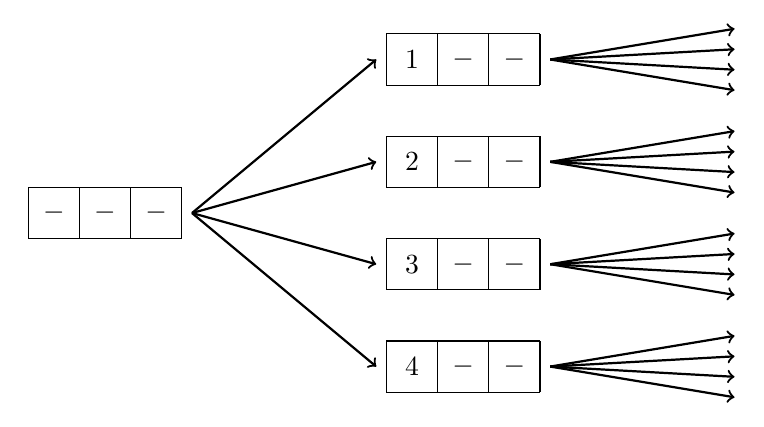
\begin{tikzpicture}[scale=.65]
    \draw (0,0) grid (3,1);
    \foreach \x/\v in {0/-,1/-,2/-} \node at (\x+0.5,0.5) {$\v$};

    \draw (7,-3) grid (10,-2);
    \foreach \x/\v in {0/1,1/-,2/-} \node at (\x+7.5,3.5) {$\v$};
    \draw (7,-1) grid (10,0);
    \foreach \x/\v in {0/2,1/-,2/-} \node at (\x+7.5,1.5) {$\v$};
    \draw (7,1) grid (10,2);
    \foreach \x/\v in {0/3,1/-,2/-} \node at (\x+7.5,-0.5) {$\v$};
    \draw (7,3) grid (10,4);
    \foreach \x/\v in {0/4,1/-,2/-} \node at (\x+7.5,-2.5) {$\v$};

    \draw[->,thick] (3.2,0.5) -- (6.8,3.5);
    \draw[->,thick] (3.2,0.5) -- (6.8,1.5);
    \draw[->,thick] (3.2,0.5) -- (6.8,-0.5);
    \draw[->,thick] (3.2,0.5) -- (6.8,-2.5);
    
    \foreach \y in {3.5,1.5,-0.5,-2.5} \foreach \z in {0.6,0.2,-0.2,-0.6}
        \draw[->,thick] (10.2,\y) -- (13.8,\y+\z);
\end{tikzpicture}
\caption{Yhdistelmien muodostaminen alkaa ($n=3$ ja $m=4$).}
\label{fig:perhak}
\end{figure}

Voimme arvioida algoritmin tehokkuutta laskemalla,
montako kertaa proseduuria \texttt{haku} kutsutaan yhteensä haun aikana.
Proseduuria kutsutaan kerran parametrilla $0$,
$m$ kertaa parametrilla $1$, $m^2$ kertaa parametrilla $2$, jne.,
joten kutsujen määrä on yhteensä
\[
1+m+m^2+\dots+m^n = \frac{m^{n+1}-1}{m-1} = O(m^n).
\]
Tästä näkee, että kutsujen yhteismäärä on samaa luokkaa kuin
viimeisen tason kutsujen määrä.
Viimeisellä tasolla tehdäänkin enemmän kutsuja kuin
kaikilla muilla tasoilla yhteensä.

\subsection{Osajoukkojen läpikäynti}

Tarkastellaan sitten ongelmaa,
jossa haluamme käydä läpi kaikki $n$ alkion
joukon \emph{osajoukot}.
Osajoukkoja on yhteensä $2^n$,
koska jokainen alkio joko kuuluu tai ei kuulu osajoukkoon.
Esimerkiksi joukon $\{2,3,5,9\}$ osajoukkoja ovat
$\{2,5\}$ ja $\{3,5,9\}$.

Osoittautuu, että voimme ratkaista tehtävän
käymällä läpi kaikki $n$ luvun yhdistelmät,
joissa jokainen luku on 0 tai 1.
Ideana on, että jokainen yhdistelmän luku kertoo,
kuuluuko tietty alkio osajoukkoon,
Alkio kuuluu osajoukkoon tarkalleen silloin,
kun sen kohdalla on luku 1.
Esimerkiksi kun joukkona on $\{2,3,5,9\}$,
yhdistelmä $[1,0,1,0]$ vastaa
osajoukkoa $\{2,5\}$ ja
yhdistelmä $[0,1,1,1]$ vastaa osajoukkoa $\{3,5,9\}$.

Seuraava koodi näyttää, miten voimme käydä osajoukot
läpi peruuttavan haun avulla.
Proseduuri \texttt{haku} valitsee,
otetaanko kohdassa $k$ oleva alkio mukaan osajoukkoon vai ei,
ja merkitsee tämän tiedon taulukkoon \texttt{valinta}.
Kuten ennenkin, haku lähtee käyntiin kutsulla \texttt{haku}$(0)$.

\begin{code}
procedure haku(k)
    if k == n
        // käsittele osajoukko
    else
        for i = 0 to 1
            valinta[k] = i
            haku(k+1)
\end{code}

\subsection{Permutaatioiden läpikäynti}

Peruuttavan haun avulla voimme myös käydä läpi joukon
\emph{permutaatiot} eli erilaiset järjestykset.
Kun joukossa on $n$ alkiota, siitä voidaan muodostaa
kaikkiaan $n!$ permutaatiota.
Esimerkiksi joukon $\{1,2,3,4\}$ permutaatioita ovat
$\{2,4,1,3\}$ ja $\{4,3,1,2\}$.

Tässä tilanteessa haluamme käydä läpi $n$ luvun yhdistelmiä,
joissa jokainen luku on väliltä $1 \dots n$
ja lisäksi mikään luku ei toistu.
Saamme tämän aikaan lisäämällä hakuun uuden taulukon
\texttt{mukana}, joka kertoo, onko tietty luku jo mukana.
Joka vaiheessa haku voi valita yhdistelmään vain sellaisia lukuja,
joita ei ole valittu siihen aiemmin.

\begin{code}
procedure haku(k)
    if k == n
        print(luvut)
    else
        for i = 1 to n
            if not mukana[i]
                mukana[i] = true
                luvut[k] = i
                haku(k+1)
                mukana[i] = false
\end{code}


\section{Esimerkki: Kuningatarongelma}

Klassinen tehtävä on selvittää,
monellako tavalla shakkilaudalle voidaan asettaa kahdeksan kuningatarta
niin, etteivät ne uhkaa toisiaan.
Käsittelemme seuraavaksi tämän tehtävän yleistystä,
jossa haluamme asettaa $n$ kuningatarta $n \times n$ -laudalle.
Esimerkiksi tapauksessa $n=4$ mahdollisia sijoitustapoja on 2,
jotka on esitetty kuvassa \ref{fig:kuning}.


\begin{figure}
\center
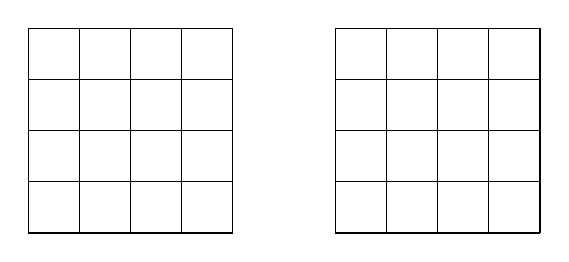
\begin{tikzpicture}[scale=.65]
  \begin{scope}
    \draw (0, 0) grid (4, 4);
    \node at (1.5,3.5) {$\symqueen$};
    \node at (3.5,2.5) {$\symqueen$};
    \node at (0.5,1.5) {$\symqueen$};
    \node at (2.5,0.5) {$\symqueen$};

    \draw (6, 0) grid (10, 4);
    \node at (6+2.5,3.5) {$\symqueen$};
    \node at (6+0.5,2.5) {$\symqueen$};
    \node at (6+3.5,1.5) {$\symqueen$};
    \node at (6+1.5,0.5) {$\symqueen$};
  \end{scope}
\end{tikzpicture}
\caption{Mahdolliset tavat asettaa 4 kuningatarta $4 \times 4$ -shakkilaudalle.}
\label{fig:kuning}
\end{figure}

\subsection{Haun toteuttaminen}

Voimme ratkaista tehtävän peruuttavalla haulla toteuttamalla algoritmin,
joka käy laudan läpi ylhäältä alaspäin ja asettaa yhden kuningattaren
jokaiselle riville.
Kuva \ref{fig:hakupuu} esittää haun toimintaa tapauksessa $n=4$.
Ensimmäisen rivin kuningatar voidaan asettaa mihin tahansa sarakkeeseen,
mutta seuraavilla riveillä aiemmat valinnat rajoittavat hakua.
Kuvassa näkyy toisen kuningattaren sijoittaminen,
kun ensimmäinen kuningatar on sarakkeessa 2.
Tällöin ainoa vaihtoehto on, että toinen kuningatar on sarakkeessa 4,
koska kaikissa muissa tapauksissa kuningattaret uhkaisivat toisiaan.


\begin{figure}
\center
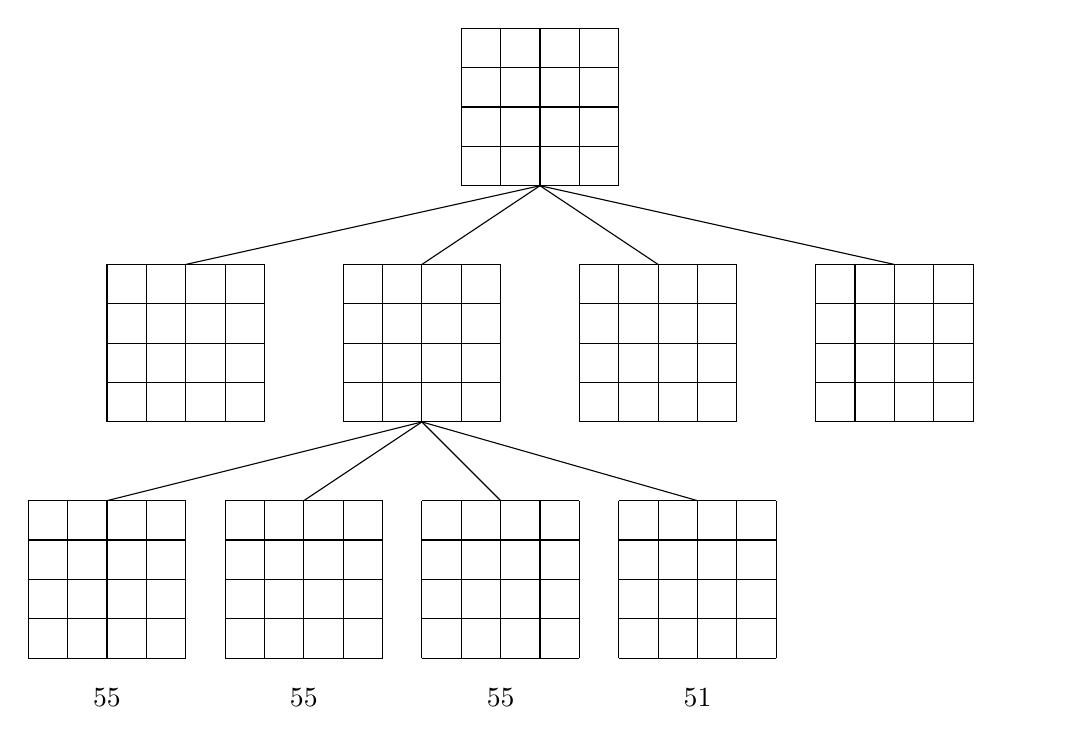
\begin{tikzpicture}[scale=.50]
  \begin{scope}
    \draw (0, 0) grid (4, 4);

    \draw (-9, -6) grid (-5, -2);
    \draw (-3, -6) grid (1, -2);
    \draw (3, -6) grid (7, -2);
    \draw (9, -6) grid (13, -2);

    \node at (-9+0.5,-3+0.5) {$\symqueen$};
    \node at (-3+1+0.5,-3+0.5) {$\symqueen$};
    \node at (3+2+0.5,-3+0.5) {$\symqueen$};
    \node at (9+3+0.5,-3+0.5) {$\symqueen$};

    \draw (2,0) -- (-7,-2);
    \draw (2,0) -- (-1,-2);
    \draw (2,0) -- (5,-2);
    \draw (2,0) -- (11,-2);

    \draw (-11, -12) grid (-7, -8);
    \draw (-6, -12) grid (-2, -8);
    \draw (-1, -12) grid (3, -8);
    \draw (4, -12) grid (8, -8);
    \draw[white] (11, -12) grid (15, -8);
    \node at (-11+1+0.5,-9+0.5) {$\symqueen$};
    \node at (-6+1+0.5,-9+0.5) {$\symqueen$};
    \node at (-1+1+0.5,-9+0.5) {$\symqueen$};
    \node at (4+1+0.5,-9+0.5) {$\symqueen$};
    \node at (-11+0+0.5,-10+0.5) {$\symqueen$};
    \node at (-6+1+0.5,-10+0.5) {$\symqueen$};
    \node at (-1+2+0.5,-10+0.5) {$\symqueen$};
    \node at (4+3+0.5,-10+0.5) {$\symqueen$};

    \draw (-1,-6) -- (-9,-8);
    \draw (-1,-6) -- (-4,-8);
    \draw (-1,-6) -- (1,-8);
    \draw (-1,-6) -- (6,-8);
    
    \node at (-9,-13) {\ding{55}};
    \node at (-4,-13) {\ding{55}};
    \node at (1,-13) {\ding{55}};
    \node at (6,-13) {\ding{51}};    
  \end{scope}
\end{tikzpicture}
\caption{Peruuttavan haun toiminta kuningatarongelmassa.}
\label{fig:hakupuu}
\end{figure}


Seuraava proseduuri \texttt{haku} esittää peruuttavan haun algoritmin,
joka etsii kuningatarongelman ratkaisut.
Oletamme, että laudan rivit ja sarakkeet on numeroitu $0,1,\dots,n-1$.
Parametri $y$ kertoo, mille riville seuraava kuningatar tulee sijoittaa,
ja haku lähtee käyntiin kutsulla \texttt{haku}$(0)$.
Jos rivinä on $n$, kaikki kuningattaret on jo sijoitettu,
joten yksi ratkaisu on löytynyt.
Muuten suoritetaan silmukka, joka käy läpi mahdolliset sarakkeet
muuttujan $x$ avulla.
Jos kuningatar voidaan sijoittaa sarakkeeseen $x$
eli se ei uhkaa mitään aiemmin sijoitettua kuningatarta,
merkitään taulukkoon \texttt{kohta},
että kuningatar $y$ on sarakkeessa $x$,
ja haku jatkuu eteenpäin rekursiivisesti.

\begin{code}
procedure haku(y)
    if y == n
        laskuri++
    else
        for x = 0 to n-1
            if voi_sijoittaa(y,x)
                kohta[y] = x
                haku(y+1)
\end{code}

Lisäksi täytyy toteuttaa funktio \texttt{voi\_sijoittaa},
joka tutkii, voidaanko uusi kuningatar sijoittaa
rivin $y$ sarakkeelle $x$.
Tämä voidaan selvittää taulukon \texttt{kohta} avulla näin:

\begin{code}
function voi_sijoittaa(y,x)
    for i = 0 to y-1
        if kohta[i] == x
            return false
        if abs(i-y) == abs(kohta[i]-x)
            return false
    return true
\end{code}

Funktio käy läpi kaikki aiemmin sijoitetut kuningattaret.
Jos aiemmin sijoitettu kuningatar olisi samassa sarakkeessa
(ensimmäinen ehto) tai samalla vinorivillä (toinen ehto)
kuin uusi kuningatar, tällaista sijoitusta ei voida tehdä
ja funktio palauttaa \texttt{false}.
Jos taas mikään aiempi kuningatar ei uhkaa uutta kuningatarta,
funktio palauttaa \texttt{true}.
Huomaa jälkimmäisessä ehdossa kätevä tapa tarkastaa,
ovatko kuningattaret samalla vinorivillä funktion \texttt{abs}
(itseisarvo) avulla.
Kuningattaret ovat samalla vinorivillä tarkalleen silloin,
kun niiden vaaka- ja pystysuuntaiset erot ovat samat.

Nyt meillä on valmis algoritmi, joiden avulla voimme etsiä
kuningatarongelman ratkaisuja.
Aina kun ratkaisu on valmis, taulukko \texttt{sarake} kertoo,
missä sarakkeissa kuningattaret ovat.
Esimerkiksi tapauksen $n=4$ ratkaisut (kuva \ref{fig:kuning})
vastaavat taulukoita $[1,3,0,2]$ ja $[2,0,3,1]$.
Voimme vaikkapa selvittää algoritmin avulla,
että tapauksessa $n=8$ eli tavallisella shakkilaudalla
ratkaisuja on yhteensä 92.

\subsection{Haun tehostaminen}

Peruuttavan haun algoritmit ovat usein hitaita,
koska ne joutuvat käymään läpi suuren määrän osittaisia ratkaisuja.
Voimme kuitenkin usein tehostaa hakua merkittävästi
toteuttamalla se paremmin.

Kuningatarongelmassa tapaus $n=8$ on vielä helppo ja
saamme laskettua tapojen määrän salamannopeasti,
mutta pian tämän jälkeen algoritmi alkaa hidastua tuntuvasti.
Tarkastelemme seuraavaksi tapausta $n=16$,
jossa sijoitustapojen määrä on 14772512.
Tässä tapauksessa yllä kuvatun algoritmin
Java-toteutus vie testikoneella aikaa 290 sekuntia.

\index{symmetria}
Yksi usein toimiva tapa tehostaa peruuttavan haun algoritmia
on ottaa huomioon \emph{symmetria}.
Kuningatarongelmassa hyödyllinen havainto on,
että jokaista ratkaisua vastaa toinen ratkaisu,
joka saadaan peilaamalla se vaakasuuntaisesti.
Niinpä voimme päättää, että asetamme ensimmäisen kuningattaren
laudan vasempaan osaan ($n/2$ ensimmäistä saraketta)
ja kerromme lopuksi vastauksen kahdella.
Tämä optimointi on hyvin helppo toteuttaa ja se puolittaa
laskenta-ajan: nyt algoritmi vie aikaa vain 145 sekuntia.

Voimme tehostaa algoritmia vielä lisää toteuttamalla
uhkaamisen tarkastuksen paremmin.
Seuraava toteutus käyttää kolmea aputaulukkoa
\texttt{uhka1}, \texttt{uhka2} ja \texttt{uhka3}.
Ensimmäinen taulukko kertoo, mitkä sarakkeet on varattu,
ja kaksi muuta taulukkoa ilmoittavat, mitkä vinorivit on varattu.
Vinorivejä kulkee kahteen suuntaan
(ylävasemmalta alaoikealle ja alavasemmalta yläoikealle)
ja ne on numeroitu $0,1,\dots,2n-2$.
Näiden taulukoiden avulla voimme tarkastaa $O(1)$-ajassa,
voimmeko sijoittaa kuningattaren tiettyyn paikkaan,
eikä tarvitse käydä läpi aiempia kuningattaria silmukalla.

\begin{code}
procedure haku(y)
    if y == n
        laskuri++
    else
        for i = 0 to n-1
            if !uhka1[x] && !uhka2[x+y] && !uhka3[x-y+n-1]
                uhka1[x] = uhka2[x+y] = uhka3[x-y+n-1] = true
                haku(y+1)
                uhka1[x] = uhka2[x+y] = uhka3[x-y+n-1] = false
\end{code}

Tämän optimoinnin jälkeen haku vie aikaa vain 62 sekuntia.
Alkuperäinen toteutus vei aikaa 290 sekuntia,
joten optimointien tulokseen voi olla tyytyväinen.
Suuremmissa tapauksissa optimoinneista tuleva hyöty olisi
luultavasti vielä suurempi.

\section{Esimerkki: Pakkaaminen}

Annettuna on $n$ tavaraa, joilla jokaisella on tietty paino.
Tehtävänä on jakaa tavarat laatikoihin niin,
että jokaisen laatikon paino on enintään $x$ ja
laatikoiden määrä on mahdollisimman pieni.
Esimerkiksi jos $n=5$, painot ovat $[2,3,3,7,8]$ ja $x=9$,
paras ratkaisu on muodostaa laatikot $[2,7]$, $[3,3]$ ja $[8]$,
jolloin tarvitaan 3 laatikkoa.

Parhaan jakotavan löytäminen on vaikea tehtävä,
johon ei tunneta mitään tehokasta algoritmia.
Voimme kuitenkin toteuttaa peruuttavan haun algoritmin,
joka käy läpi kaikki mahdolliset ratkaisut.

\subsection{Haun toteuttaminen}

Tässä tehtävässä on monta luontevaa tapaa toteuttaa
peruuttavan haun algoritmi.
Seuraavassa toteutuksessa proseduuri \texttt{haku} saa kaksi parametria:
$k$ kertoo, mikä tavara pakataan seuraavaksi,
ja $c$ kertoo, montako laatikkoa on jo käytössä.
Haku lähtee käyntiin kutsulla \texttt{haku}$(0,0)$.
Taulukko \texttt{paino} kertoo jokaisen tavaran painon,
ja taulukko \texttt{summa} sisältää puolestaan
jokaisesta laatikosta siinä olevien tavaroiden painojen summan.
Lisäksi muuttujassa $p$ on laatikoiden määrä pienimmässä ratkaisussa
tähän mennessä.
Tämän muuttujan arvona on alussa $\infty$,
koska mitään ratkaisua ei ole vielä löytynyt.

\begin{code}
procedure haku(k,c)
    if k == n
        p = min(p,c)
        return
    for i = 0 to c-1
        if summa[i]+paino[k] <= x
            summa[i] += paino[k]
            haku(k+1,c)
            summa[i] -= paino[k]
    summa[c] = paino[k]
    haku(k+1,c+1)
\end{code}

Jos $k=n$, jokin ratkaisu on löytynyt ja $c$ sisältää
laatikoiden määrän tässä ratkaisussa.
Tässä vaiheessa muuttuja $p$ päivittyy,
jos uusi ratkaisu on aiempaa pienempi.
Jos ratkaisu ei ole valmis, haku käy läpi kaikki
nykyiset laatikot ja koettaa jokaisen laatikon
kohdalla pakata seuraavan tavaran sinne.
Jos tavara mahtuu laatikkoon,
se lisätään sinne ja haku jatkuu rekursiivisesti.
Tämän jälkeen tavara poistetaan laatikosta.
Lopuksi käsitellään vielä tapaus, jossa tavara laitetaan
uuteen laatikkoon, jolloin $c$ kasvaa yhdellä.

\subsection{Haun tehostaminen}

Yllä kuvattu algoritmi on toimiva, mutta \emph{hyvin hidas},
koska se käy läpi valtavan määrän ratkaisuja.
Käytännössä monet ratkaisut ovat huonoja, koska niissä on
paljon laatikoita, jotka jäävät tyhjilleen.
Voimmekin tehostaa algoritmia huomattavasti keskeyttämällä
ratkaisun muodostamisen, jos on selvää, ettei siitä voi
tulla aiemmin löydettyä ratkaisua parempi.

Koska muistissa on aina laatikoiden määrä parhaassa
löydetyssä ratkaisussa ($p$),
saamme tästä \emph{ylärajan} sille, montako laatikkoa tarvitaan.
Toisaalta laatikoiden määrä nykyisessä ratkaisussa ($c$) on
\emph{alaraja} sille, montako laatikkoa muodosteilla oleva
ratkaisu tulee sisältämään.
Jos alaraja on yhtä suuri tai suurempi kuin yläraja,
emme voi saada aiempaa parempaa ratkaisua,
joten ei kannata jatkaa ratkaisun muodostamista.
Tämä onnistuu lisäämällä algoritmin alkuun seuraava tarkastus:

\begin{code}
procedure haku(k,c)
    if c >= p
        return
    ...
\end{code}

Tämä on jo merkittävä tehostus, mutta voimme vielä parantaa
alarajaa, koska voimme arvioida, montako laatikkoa
lisää ainakin vielä tarvitaan. Tämä selviää kaavalla
\[
\frac{s_T-s_L}{x},
\]
missä $s_T$ on vielä lisäämättä olevien tavaroiden yhteispaino ja
$s_L$ kertoo, miten paljon painoa nykyisiin laatikoihin
voisi vielä laittaa lisää.
Niinpä $s_T-s_L$ ilmaisee, miten paljon painoa meidän täytyy
laittaa varmasti uusiin laatikoihin.
Ihannetilanteessa jokaiseen laatikkoon tulee painoa $x$,
joten saamme kaavasta alarajan sille, montako laatikkoa tarvitaan vielä.
Voimme luoda kaavasta funktion \texttt{arvio},
jonka voi yhdistää hakuun näin:

\begin{code}
procedure haku(k,c)
    if c+arvio(k,c) >= p
        return
    ...
\end{code}

\index{branch and bound}
Nyt meillä on aiempaa parempi alaraja tarvittavien laatikoiden määrälle,
koska laskemme yhteen, montako laatikkoa on jo käytetty ja montako
tarvitaan vielä lisää.

\index{branch and bound}
Tällaista peruuttavan haun toteutusta kutsutaan joskus nimellä
\emph{branch and bound}.
Tässä \emph{branch} tarkoittaa, että haku haarautuu,
ja \emph{bound} viittaa siihen, että haku hyödyntää
ylä- ja alarajoja.

\section{Pelin tekoäly}

\subsection{Minmax-algoritmi}

\subsection{Alfa-beta-karsinta}

\chapter{Dynaaminen ohjelmointi}

Dynaaminen ohjelmointi on algoritmisuunnittelun tekniikka,
jota voi käyttää kahdenlaisissa tilanteissa:

\begin{itemize}
\item \textbf{Optimiratkaisun etsiminen}: Haluamme etsiä ratkaisun,
joka on jollakin tavalla suurin tai pienin.
\item \textbf{Ratkaisumäärän laskeminen}: Haluamme laskea,
montako erilaista ratkaisua on olemassa.
\end{itemize}

Ideana on muotoilla laskentatehtävä
rekursiivisesti niin, että voimme ratkaista tehtävän
ratkaisemalla ensin osatehtävinä saman tehtävän pienempiä tapauksia.
Aina kun olemme ratkaisseet tietyn osatehtävän,
kirjaamme sen ratkaisun muistiin, minkä ansiosta
pystymme hakemaan ratkaisun tehokkaasti uudestaan,
kun tarvitsemme sitä myöhemmin.

Tässä luvussa tutustumme ensin dynaamisen ohjelmoinnin perusteisiin
käyttäen esimerkkinä tehtävää, jossa haluamme laskea,
monellako tavalla voimme rakentaa tornin palikoista.
Tämän jälkeen käymme läpi joukon muita tehtäviä, jotka esittelevät
dynaamisen ohjelmoinnin mahdollisuuksia.

\section{Perustekniikat}

Aloitamme dynaamiseen ohjelmointiin tutustumisen
seuraavasta tehtävästä:
meillä on palikoita, joiden korkeudet ovat 1, 2 ja 3,
ja haluamme rakentaa niistä tornin, jonka korkeus on $n$.
Jokaista palikkatyyppiä on saatavilla rajattomasti.
Monellako tavalla voimme rakentaa tornin?

\begin{figure}
\center
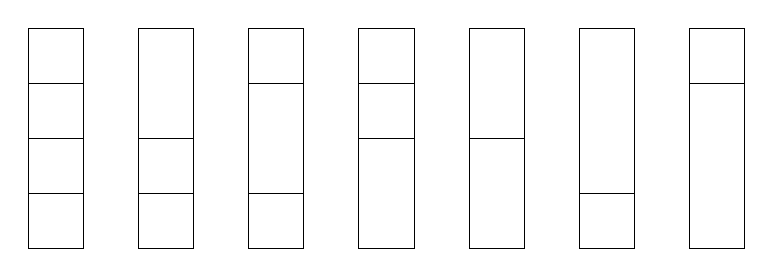
\begin{tikzpicture}[scale=0.7]
\newcommand\palikka[3]{
\draw (2*#1,#2) rectangle (2*#1+1,#2+#3);
}
%\foreach \i in {0,1,...,6} \draw (2*\i,0) grid (2*\i+1,4);
\palikka{0}{0}{1} \palikka{0}{1}{1} \palikka{0}{2}{1} \palikka{0}{3}{1}
\palikka{1}{0}{1} \palikka{1}{1}{1} \palikka{1}{2}{2}
\palikka{2}{0}{1} \palikka{2}{1}{2} \palikka{2}{3}{1}
\palikka{3}{0}{2} \palikka{3}{2}{1} \palikka{3}{3}{1}
\palikka{4}{0}{2} \palikka{4}{2}{2}
\palikka{5}{0}{1} \palikka{5}{1}{3}
\palikka{6}{0}{3} \palikka{6}{3}{1}
\end{tikzpicture}
\caption{Voimme rakentaa korkeuden 4 tornin 7 tavalla palikoista,
joiden korkeudet ovat 1, 2 ja 3.}
\label{fig:dyntor}
\end{figure}

Kuva \ref{fig:dyntor} näyttää esimerkin, jossa $n=4$.
Tässä esimerkissä meillä on 7 tapaa rakentaa torni palikoista.
Voimme luonnehtia torneja myös summina luvuista 1, 2 ja 3.
Tässä tapauksessa vasen torni vastaa summaa $1+1+1+1$,
seuraava torni vastaa summaa $1+1+2$, jne.

Jos $n$ on pieni, voimme laskea tornien määrän helposti
käymällä läpi kaikki tavat, mutta tornien määrä kasvaa
nopeasti emmekä voi käyttää raakaa voimaa suuremmilla
$n$:n arvoilla.
Seuraavaksi ratkaisemmekin ongelman tehokkaasti
dynaamisen ohjelmoinnin avulla.

\subsection{Rekursiivinen esitys}

Jotta voimme käyttää dynaamista ohjelmointia,
meidän täytyy esittää ongelma rekursiivisesti
niin, että saamme laskettua ongelman ratkaisun
käyttäen osaongelmina pienempiä vastaavia ongelmia.

Tässä tehtävässä meidän on luontevaa määritellä rekursiivinen
funktio $\texttt{tornit}(n)$: monellako tavalla voimme
rakentaa tornin, jonka korkeus on $n$?
Esimerkiksi $\texttt{tornit}(4)=7$, koska tiedämme
esimerkkimme ansiosta,
että voimme rakentaa korkeuden 4 tornin 7 tavalla.

Funktion pienten arvojen laskeminen on helppoa.
Ensinnäkin $\texttt{tornit}(0)=1$, koska voimme
muodostaa tyhjän tornin yhdellä tavalla:
siinä ei ole mitään palikoita.
Sitten $\texttt{tornit}(1)=1$, koska ainoa mahdollisuus
on valita korkeuden 1 palikka,
ja $\texttt{tornit}(2)=2$, koska voimme joko valita
kaksi korkeuden 1 palikkaa tai yhden korkeuden 2 palikan.

\begin{figure}
\center
\begin{tikzpicture}[scale=0.7]
\draw (0,0) rectangle (1,1);
\draw[dashed] (0,1) rectangle (1,4);
\draw (4,0) rectangle (5,2);
\draw[dashed] (4,2) rectangle (5,4);
\draw (8,0) rectangle (9,3);
\draw[dashed] (8,3) rectangle (9,4);
\draw [decorate,decoration={brace,amplitude=4pt},xshift=0.2cm] (1,4) -- (1,1) node [midway,right,xshift=.1cm] {$n-1$};
\draw [decorate,decoration={brace,amplitude=4pt},xshift=0.2cm] (5,4) -- (5,2) node [midway,right,xshift=.1cm] {$n-2$};
\draw [decorate,decoration={brace,amplitude=4pt},xshift=0.2cm] (9,4) -- (9,3) node [midway,right,xshift=.1cm] {$n-3$};
\end{tikzpicture}
\caption{Rekursiivinen idea: kun alamme rakentaa tornia, voimme laittaa pohjalle
korkeuden 1, 2 tai 3 palikan.}
\label{fig:dynrek}
\end{figure}


Kuinka voisimme sitten laskea funktion arvon yleisessä tapauksessa,
kun tornin korkeus on $n$?
Tässä voimme miettiä, kuinka tornin rakentaminen alkaa.
Meillä on kolme mahdollisuutta: voimme laittaa ensin palikan
korkeutta 1, 2 tai 3.
Jos valitsemme korkeuden 1 palikan, meidän täytyy rakentaa
sen päälle korkeuden $n-1$ torni.
Vastaavasti jos valitsemme korkeuden 2 tai 3 palikan,
meidän täytyy rakentaa sen päälle torni,
jonka korkeus on $n-2$ tai $n-3$.
Kuva \ref{fig:dynrek} havainnollistaa tämän idean.

Niinpä voimme laskea tornien määrän rekursiivisesti kaavalla
\[
\texttt{tornit}(n) = \texttt{tornit}(n-3)+\texttt{tornit}(n-2)+\texttt{tornit}(n-1),
\]
kun $n \ge 3$.
Esimerkiksi voimme laskea
\[
\texttt{tornit}(3) = \texttt{tornit}(0)+\texttt{tornit}(1)+\texttt{tornit}(2)=4
\]
ja
\[
\texttt{tornit}(4) = \texttt{tornit}(1)+\texttt{tornit}(2)+\texttt{tornit}(3)=7,
\]
jolloin olemme saaneet laskettua esimerkkitapaustamme vastaavasti,
että voimme rakentaa korkeuden 4 tornin 7 tavalla.

\begin{table}
\center
\begin{tabular}{rrr}
korkeus $n$ & $\texttt{tornit}(n)$ \\
\hline
0 & 1 \\
1 & 1 \\
2 & 2 \\
3 & 4 \\
4 & 7 \\
5 & 13 \\
6 & 24 \\
7 & 44 \\
8 & 81 \\
9 & 149 \\
\end{tabular}
\caption{Tornien määrät, kun korkeus $n$ on $0,1,\dots,9$.}
\label{tab:dyntor}
\end{table}

Taulukko \ref{tab:dyntor} näyttää yhteenvedon funktion
$\texttt{tornit}(n)$ arvoista, kun $n=0,1,\dots,9$.
Kuten taulukosta voi huomata, funktion arvo kasvaa nopeasti:
se lähes kaksinkertaistuu joka askeleella.
Kun $n$ on suuri,
meillä onkin valtavasti mahdollisuuksia tornin rakentamiseen.

\subsection{Tehokas toteutus}

Nyt kun olemme saaneet aikaan rekursiivisen funktion,
voimme toteuttaa sen ohjelmoimalla seuraavasti:

\begin{code}
long tornit(int n) {
    if (n == 0) return 1;
    if (n == 1) return 1;
    if (n == 2) return 2;
    return tornit(n-3)+tornit(n-2)+tornit(n-1);
}
\end{code}

Tämä on toimiva ratkaisu, mutta siinä on yksi ongelma:
funktion arvon laskeminen vie kauan aikaa, jos $n$ on
vähänkin suurempi.
Käytännössä laskenta alkaa hidastua parametrin $n=30$ tienoilla.
Esimerkiksi arvon $\texttt{tornit}(40)$ laskeminen vie aikaa
jo useita minuutteja, ja voimme arvioida, että
arvon $\texttt{tornit}(50)$ laskeminen veisi aikaa noin vuorokauden.

Syynä laskennan hitauteen on, että metodia $\texttt{tornit}$
kutsutaan uudestaan ja uudestaan samoilla parametreilla
ja tornien määrä lasketaan loppujen lopuksi summana
luvuista 1 ja 2 pohjatapauksista.
Niinpä kun tornien määrä on suuri,
laskenta on tuomittu viemään kauan aikaa.
Voimme kuitenkin selviytyä ongelmasta toteuttamalla
laskennan hieman toisella tavalla.

Tässä astuu kuvaan dynaamisen ohjelmoinnin keskeinen idea:
laskemme funktion arvon kullekin parametrille vain kerran
ja tallennamme tulokset taulukkoon myöhempää käyttöä varten.
Tätä varten luomme taulukon $\texttt{tornit}$,
jossa kohtaan $\texttt{tornit}[i]$ tallennetaan funktion
arvo $\texttt{tornit}(i)$.
Kun haluamme laskea korkeuden $n$ tornien määrän,
täytämme taulukon kohdat $0,1,\dots,n$.
Seuraava koodi toteuttaa laskennan:

\begin{code}
long[] tornit = new long[n+1];
tornit[0] = 1;
tornit[1] = 1;
tornit[2] = 2;
for (int i = 3; i <= n; i++) {
    tornit[i] = tornit[i-3]+tornit[i-2]+tornit[i-1];
}
\end{code}

Koodin suorituksen jälkeen taulukon arvo $\texttt{tornit}[n]$
kertoo meille, monellako tavalla voimme rakentaa
korkeuden $n$ tornin.

Tämän toteutuksen etuna on, että se on huomattavasti
nopeampi kuin rekursiivinen metodi.
Koska koodissa on vain yksi for-silmukka, se vie aikaa
vain $O(n)$, eli voimme käsitellä tehokkaasti myös
suuria $n$:n arvoja.
Esimerkiksi voimme nyt laskea salamannopeasti, että
\[
\texttt{tornit}(50) = 10562230626642,
\]
eli meillä on yli 10562 miljardia tapaa rakentaa korkeuden 50 torni.

\section{Esimerkkejä}

Olemme nyt tutustuneet dynaamisen ohjelmoinnin perusideaan,
mutta tämä on vasta alkua sille, mitä kaikkea tekniikan
avulla pystyy tekemään.
Seuraavaksi käymme läpi joukon tehtäviä,
jotka esittelevät lisää dynaamisen ohjelmoinnin mahdollisuuksia.

Jotta voimme käyttää dynaamista ohjelmointia ongelman
ratkaisemiseen, meidän täytyy pystyä muotoilemaan ongelma
rekursiivisesti niin, että voimme tallentaa muistiin
jokaisen osaongelman ratkaisun.
Käytännössä haasteena on keksiä, mikä on hyvä rekursiivinen
muotoilu ongelmalle.

\subsection{Pisin nouseva alijono}

Ensimmäinen ongelmamme on selvittää, kuinka pitkä on
$n$ alkiota sisältävän taulukon \emph{pisin nouseva alijono}.
Tämä tarkoittaa, että meidän tulee valita taulukosta
mahdollisimman pitkä jono alkioita niin,
että seuraava alkio on aina edellistä suurempi.
Kuvassa \ref{fig:pisnou} on esimerkki taulukosta,
jonka pisin nouseva alijono $[2,5,7,8]$ on pituudeltaan 4.

\begin{figure}
\center
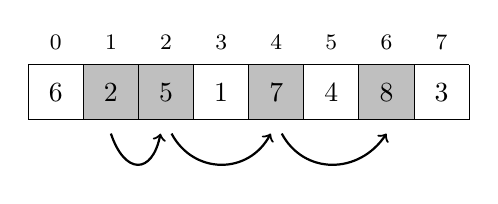
\begin{tikzpicture}[scale=0.7]
\fill[color=lightgray] (1,0) rectangle (2,1);
\fill[color=lightgray] (2,0) rectangle (3,1);
\fill[color=lightgray] (4,0) rectangle (5,1);
\fill[color=lightgray] (6,0) rectangle (7,1);
\draw (0,0) grid (8,1);
\node at (0.5,0.5) {$6$};
\node at (1.5,0.5) {$2$};
\node at (2.5,0.5) {$5$};
\node at (3.5,0.5) {$1$};
\node at (4.5,0.5) {$7$};
\node at (5.5,0.5) {$4$};
\node at (6.5,0.5) {$8$};
\node at (7.5,0.5) {$3$};
\draw[thick,->] (1.5,-0.25) .. controls (1.75,-1.00) and (2.25,-1.00) .. (2.4,-0.25);
\draw[thick,->] (2.6,-0.25) .. controls (3.0,-1.00) and (4.0,-1.00) .. (4.4,-0.25);
\draw[thick,->] (4.6,-0.25) .. controls (5.0,-1.00) and (6.0,-1.00) .. (6.5,-0.25);
\footnotesize
\node at (0.5,1.4) {$0$};
\node at (1.5,1.4) {$1$};
\node at (2.5,1.4) {$2$};
\node at (3.5,1.4) {$3$};
\node at (4.5,1.4) {$4$};
\node at (5.5,1.4) {$5$};
\node at (6.5,1.4) {$6$};
\node at (7.5,1.4) {$7$};
\end{tikzpicture}
\caption{Taulukon pisin nouseva alijono on $[2,5,7,8]$.}
\label{fig:pisnou}
\end{figure}

Voimme lähestyä tehtävää laskemalla jokaiselle taulukon
kohdalle $k=0,1,\dots,n-1$ arvon $\texttt{pisin}(k)$:
kuinka pitkä on pisin nouseva alijono, joka päättyy kohtaan $k$.
Kun olemme laskeneet kaikki nämä arvot, suurin arvoista kertoo meille,
kuinka pitkä on pisin nouseva alijono koko taulukossa.
Esimerkiksi kuvan \ref{fig:pisnou} taulukossa $\texttt{pisin}(6)=4$,
koska kohtaan $6$ päättyvä pisin nouseva alijono on pituudeltaan $4$.

Millainen on sitten pisin kohtaan $k$ päättyvä alijono?
Yksi mahdollisuus on, että alijonossa on vain kohdan $k$ alkio,
jolloin $\texttt{pisin}(k)=1$.
Muussa tapauksessa alijono muodostuu niin,
että siinä on ensin kohtaan $x$ päättyvä
pisin nouseva alijono, missä $x<k$, ja sitten vielä kohdan $k$ alkio.
Tämä edellyttää, että kohdan $x$ alkio on pienempi
kuin kohdan $k$ alkio.
Tuloksena olevan alijonon pituus on $\texttt{pituus}(x)+1$.
Voimmekin käydä läpi kaikki mahdolliset tavat valita kohta $x$
ja ottaa niistä parhaan vaihtoehdon.

Seuraava koodi laskee jokaiselle $k=0,1,\dots,n-1$
pisimmän kohtaan $k$ päättyvän alijonon pituuden yllä kuvattua
ideaa käyttäen.
Koodi olettaa, että taulukon sisältö on taulukossa \texttt{taulu},
ja se muodostaa taulukon \texttt{pisin}, jossa on pisimpien
alijonojen pituudet.

\begin{code}
for (int k = 0; k < n; k++) {
    pisin[k] = 1;
    for (int x = 0; x < k; x++) {
        if (taulu[x] < taulu[k] && pisin[x]+1 > pisin[k]) {
            pisin[k] = pisin[x]+1;
        }
    }
}
\end{code}

Koodin suorituksen jälkeen pisimmän nousevan alijonon pituus on
siis suurin taulukon \texttt{pisin} arvoista.
Tämä algoritmi vie aikaa $O(n^2)$, koska siinä on kaksi
sisäkkäistä silmukkaa.

Mitä jos haluaisimme myös laskennan jälkeen selvittää, mistä alkioista
pisin nouseva alijono muodostuu? Tämä onnistuu laajentamalla hieman koodia.
Ideana on rakentaa taulukko \texttt{aiempi},
joka kertoo jokaisessa kohdassa, missä on tähän kohtaan
päättyvän pisimmän alijonon edellinen alkio.
Voimme muodostaa taulukon seuraavasti:

\begin{code}
for (int k = 0; k < n; k++) {
    pisin[k] = 1;
    aiempi[k] = -1;
    for (int x = 0; x < k; x++) {
        if (taulu[x] < taulu[k] && pisin[x]+1 > pisin[k]) {
            pisin[k] = pisin[x]+1;
            aiempi[k] = x;
        }
    }
}
\end{code}

Tämän jälkeen jokaisessa kohdassa $k$ arvo $\texttt{aiempi}[k]$
kertoo pisimmän alijonon edellisen alkion kohdan.
Kuitenkin jos alijonon pituus on 1, taulukossa on arvo $-1$.
Voimme selvittää kohtaan $k$ päättyvän alijonon alkiot
käänteisesti seuraavasti:

\begin{code}
while (k != -1) {
    print(taulu[k]);
    k = aiempi[k];
}
\end{code}

Voimme käyttää vastaavaa tekniikkaa
dynaamisessa ohjelmoinnissa aina, kun haluamme
selvittää, miten voimme muodostaa parhaan ratkaisun.

\subsection{Reitti ruudukossa}

\subsection{Repunpakkaus}
\chapter{Verkkojen perusteet}

\section{Verkkojen perusteet}

\section{Läpikäynti}

\subsection{Syvyyshaku}

\subsection{Leveyshaku}


\chapter{Reitinhaku}

\section{Bellman–Fordin algoritmi}

\section{Dijsktran algoritmi}

\section{Floyd-Warshallin algoritmi}

\chapter{Syklittömät verkot}

Verkon käsittelyssä keskeinen haaste ovat verkossa olevat syklit.
Jos voimme olettaa, että verkossa ei ole syklejä,
voimme ratkaista monia ongelmia helpommin kuin yleisissä verkoissa,
joissa saattaa olla syklejä.

Tässä luvussa keskitymme verkkoihin, jotka ovat suunnattuja
ja syklit\-tömiä.
Englanniksi tällaisia verkkoja kutsutaan usein nimellä \emph{dag},
joka tulee sanoista \emph{directed acyclic graph}.
Tässä tapauksessa voimme muodostaa verkolle topologisen
järjestyksen ja käyttää sen jälkeen dynaamista ohjelmointia
verkko-ongelmien ratkaisemiseen.

\section{Topologinen järjestys}

Suunnatun verkon \emph{topologinen järjestys} on solmujen järjestys,
jossa pätee, että jos solmusta $a$ on kaari solmuun $b$,
niin solmu $a$ on ennen solmua $b$ järjestyksessä.
Topologinen järjestys voidaan esittää listana,
joka sisältää kaikki verkon solmut sopivassa järjestyksessä.

\begin{figure}
\center
\begin{center}
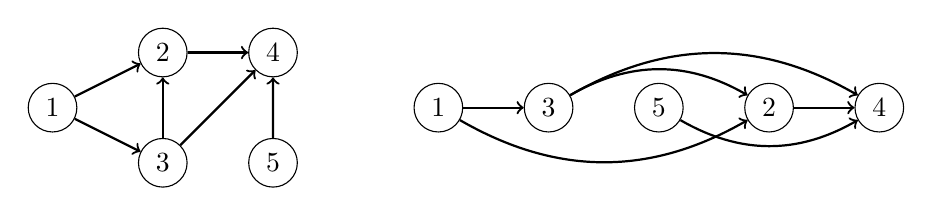
\begin{tikzpicture}[scale=0.7]
\begin{scope}
\node[draw, circle] (1) at (0,-1) {$1$};
\node[draw, circle] (2) at (2,0) {$2$};
\node[draw, circle] (3) at (2,-2) {$3$};
\node[draw, circle] (4) at (4,0) {$4$};
\node[draw, circle] (5) at (4,-2) {$5$};
\path[draw,thick,->] (1) -- (2);
\path[draw,thick,->] (1) -- (3);
\path[draw,thick,->] (3) -- (2);
\path[draw,thick,->] (2) -- (4);
\path[draw,thick,->] (3) -- (4);
\path[draw,thick,->] (5) -- (4);
\end{scope}
\begin{scope}[xshift=7cm]
\node[draw, circle] (1) at (0,-1) {$1$};
\node[draw, circle] (3) at (2,-1) {$3$};
\node[draw, circle] (5) at (4,-1) {$5$};
\node[draw, circle] (2) at (6,-1) {$2$};
\node[draw, circle] (4) at (8,-1) {$4$};
\path[draw,thick,->] (1) edge [bend right] (2);
\path[draw,thick,->] (1) -- (3);
\path[draw,thick,->] (3) edge [bend left] (2);
\path[draw,thick,->] (2) -- (4);
\path[draw,thick,->] (3) edge [bend left] (4);
\path[draw,thick,->] (5) edge [bend right] (4);
\end{scope}
\end{tikzpicture}
\end{center}
\caption{Verkko ja yksi sen topologinen järjestys $[1,3,5,2,4]$.}
\label{fig:topjar}
\end{figure}

Kuvassa \ref{fig:topjar} on esimerkkinä verkko ja yksi sen topologinen
järjestys $[1,3,5,2,4]$.
Huomaa, että verkolla on usein monta mahdollista
topologista järjestystä.
Esimerkiksi tässä verkossa myös $[5,1,3,2,4]$,
$[1,5,3,2,4]$ ja $[1,3,2,5,4]$
ovat topologisia järjestyksiä, koska voimme valita monella tavalla,
missä vaiheessa solmu $5$ on järjestyksessä.

Jos suunnattu verkko on syklitön, voimme muodostaa sille
aina topologisen järjestyksen.
Toisaalta jos verkossa on sykli,
topologista järjestystä ei voi olla olemassa,
koska emme voi valita mitään syklissä olevaa solmua
järjestykseen ennen toista.
Seuraavaksi tutustumme algoritmiin,
jonka avulla voimme muodostaa topologisen järjestyksen
tai todeta, että verkossa on sykli eikä järjestys ole mahdollinen.

\subsection{Järjestyksen muodostaminen}

Voimme muodostaa topologisen järjestyksen käyttämällä
muunnettua syvyyshakua, jossa jokaisella solmulla on kolme tilaa:

\begin{itemize}
\item tila 0 (valkoinen): solmussa ei ole käyty
\item tila 1 (harmaa): solmun käsittely on kesken
\item tila 2 (musta): solmun käsittely on valmis
\end{itemize}

\begin{figure}
\center
\begin{center}
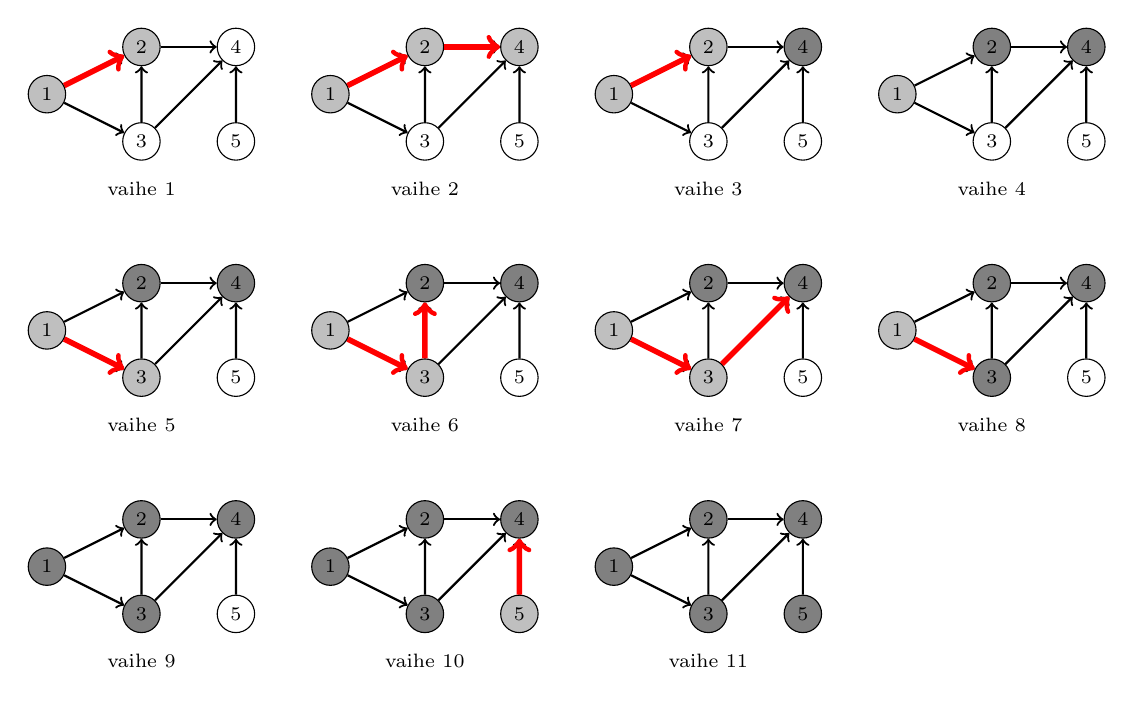
\begin{tikzpicture}[scale=0.6]
\scriptsize
\newcommand\verkko[6]{
\node[draw, circle, fill=#2] (1) at (0,-1) {$1$};
\node[draw, circle, fill=#3] (2) at (2,0) {$2$};
\node[draw, circle, fill=#4] (3) at (2,-2) {$3$};
\node[draw, circle, fill=#5] (4) at (4,0) {$4$};
\node[draw, circle, fill=#6] (5) at (4,-2) {$5$};
\path[draw,thick,->] (1) -- (2);
\path[draw,thick,->] (1) -- (3);
\path[draw,thick,->] (3) -- (2);
\path[draw,thick,->] (2) -- (4);
\path[draw,thick,->] (3) -- (4);
\path[draw,thick,->] (5) -- (4);
\node at (2,-3) {vaihe #1};
}
\begin{scope}
\verkko{1}{lightgray}{lightgray}{white}{white}{white}
\path[draw=red,thick,->,line width=2pt] (1) -- (2);
\end{scope}
\begin{scope}[xshift=6cm]
\verkko{2}{lightgray}{lightgray}{white}{lightgray}{white}
\path[draw=red,thick,->,line width=2pt] (1) -- (2);
\path[draw=red,thick,->,line width=2pt] (2) -- (4);
\end{scope}
\begin{scope}[xshift=12cm]
\verkko{3}{lightgray}{lightgray}{white}{gray}{white}
\path[draw=red,thick,->,line width=2pt] (1) -- (2);
\end{scope}
\begin{scope}[xshift=18cm]
\verkko{4}{lightgray}{gray}{white}{gray}{white}
\end{scope}
\begin{scope}[yshift=-5cm]
\verkko{5}{lightgray}{gray}{lightgray}{gray}{white}
\path[draw=red,thick,->,line width=2pt] (1) -- (3);
\end{scope}
\begin{scope}[yshift=-5cm,xshift=6cm]
\verkko{6}{lightgray}{gray}{lightgray}{gray}{white}
\path[draw=red,thick,->,line width=2pt] (1) -- (3);
\path[draw=red,thick,->,line width=2pt] (3) -- (2);
\end{scope}
\begin{scope}[yshift=-5cm,xshift=12cm]
\verkko{7}{lightgray}{gray}{lightgray}{gray}{white}
\path[draw=red,thick,->,line width=2pt] (1) -- (3);
\path[draw=red,thick,->,line width=2pt] (3) -- (4);
\end{scope}
\begin{scope}[yshift=-5cm,xshift=18cm]
\verkko{8}{lightgray}{gray}{gray}{gray}{white}
\path[draw=red,thick,->,line width=2pt] (1) -- (3);
\end{scope}
\begin{scope}[yshift=-10cm]
\verkko{9}{gray}{gray}{gray}{gray}{white}
\end{scope}
\begin{scope}[yshift=-10cm,xshift=6cm]
\verkko{10}{gray}{gray}{gray}{gray}{lightgray}
\path[draw=red,thick,->,line width=2pt] (5) -- (4);
\end{scope}
\begin{scope}[yshift=-10cm,xshift=12cm]
\verkko{11}{gray}{gray}{gray}{gray}{gray}
\end{scope}
\end{tikzpicture}
\end{center}
\caption{Esimerkki topologisen järjestyksen muodostamisesta.}
\label{fig:topesi}
\end{figure}

Algoritmin alussa jokainen solmu on valkoinen.
Käymme läpi kaikki verkon solmut ja aloitamme aina syvyyshaun
solmusta, jos se on valkoinen.
Aina kun saavumme uuteen solmuun, sen väri muuttuu
valkoisesta harmaaksi.
Sitten kun olemme käsitelleet kaikki solmusta lähtevät
kaaret, sen väri muuttuu harmaasta mustaksi.

Algoritmin aikana luomme listan, johon lisäämme solmun
aina silloin, kun sen väri muuttuu mustaksi.
Tämä lista käänteisessä järjestyksessä on verkon
topologinen järjestys.
Kuitenkin jos saavumme jossain vaiheessa uudestaan harmaaseen solmuun,
verkossa on sykli eikä topologista järjestystä voi muodostaa.

Kuva \ref{fig:topesi} näyttää, kuinka algoritmi muodostaa topologisen
järjestyksen esimerkkiverkossamme.
Tässä tapauksessa syvyyshakuja on kaksi,
joista ensimmäinen alkaa solmusta 1 ja toinen alkaa solmusta 5.
Algoritmin tuloksena on lista $[4,2,3,1,5]$,
joten käänteinen lista $[5,1,3,2,4]$ on verkon topologinen järjestys.

\begin{figure}
\center
\begin{center}
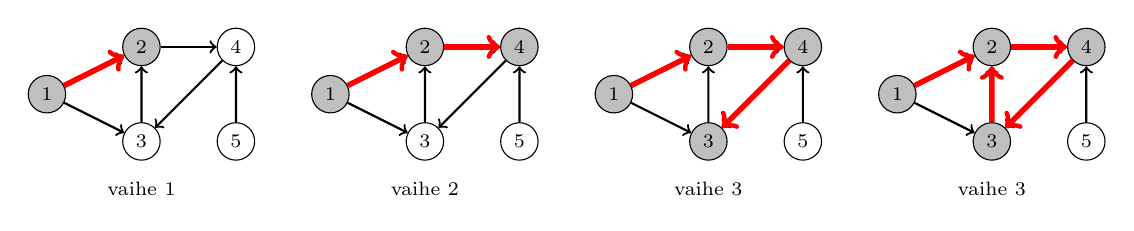
\begin{tikzpicture}[scale=0.6]
\scriptsize
\newcommand\verkko[6]{
\node[draw, circle, fill=#2] (1) at (0,-1) {$1$};
\node[draw, circle, fill=#3] (2) at (2,0) {$2$};
\node[draw, circle, fill=#4] (3) at (2,-2) {$3$};
\node[draw, circle, fill=#5] (4) at (4,0) {$4$};
\node[draw, circle, fill=#6] (5) at (4,-2) {$5$};
\path[draw,thick,->] (1) -- (2);
\path[draw,thick,->] (1) -- (3);
\path[draw,thick,->] (3) -- (2);
\path[draw,thick,->] (2) -- (4);
\path[draw,thick,->] (4) -- (3);
\path[draw,thick,->] (5) -- (4);
\node at (2,-3) {vaihe #1};
}
\begin{scope}
\verkko{1}{lightgray}{lightgray}{white}{white}{white}
\path[draw=red,thick,->,line width=2pt] (1) -- (2);
\end{scope}
\begin{scope}[xshift=6cm]
\verkko{2}{lightgray}{lightgray}{white}{lightgray}{white}
\path[draw=red,thick,->,line width=2pt] (1) -- (2);
\path[draw=red,thick,->,line width=2pt] (2) -- (4);
\end{scope}
\begin{scope}[xshift=12cm]
\verkko{3}{lightgray}{lightgray}{lightgray}{lightgray}{white}
\path[draw=red,thick,->,line width=2pt] (1) -- (2);
\path[draw=red,thick,->,line width=2pt] (2) -- (4);
\path[draw=red,thick,->,line width=2pt] (4) -- (3);
\end{scope}
\begin{scope}[xshift=18cm]
\verkko{3}{lightgray}{lightgray}{lightgray}{lightgray}{white}
\path[draw=red,thick,->,line width=2pt] (1) -- (2);
\path[draw=red,thick,->,line width=2pt] (2) -- (4);
\path[draw=red,thick,->,line width=2pt] (4) -- (3);
\path[draw=red,thick,->,line width=2pt] (3) -- (2);
\end{scope}
\end{tikzpicture}
\end{center}
\caption{Topologista järjestystä ei voi muodostaa syklin takia.}
\label{fig:topsyk}
\end{figure}

Kuva \ref{fig:topsyk} näyttää puolestaan esimerkin tilanteesta,
jossa topologista järjestystä ei voi muodostaa verkossa
olevan syklin takia.
Tässä verkossa on sykli $2 \rightarrow 4 \rightarrow 3 \rightarrow 2$,
jonka olemassaolon huomaamme siitä, että tulemme uudestaan
harmaaseen solmuun 2.

Algoritmin toiminta vastaa syvyyshakua, joten se vie aikaa $O(n+m)$.

\subsection{Miksi algoritmi toimii?}

Miten voimme tietää, että tässä kuvattu algoritmi toimii
oikein kaikissa mahdollisissa tilanteissa?

Tarkastellaan ensin tilannetta, jossa verkossa on sykli.
Jos algoritmi saapuu uudestaan harmaaseen solmuun $x$,
on selvää, että verkossa on sykli,
koska algoritmi on onnistunut pääsemään solmusta $x$
takaisin itseensä kulkemalla jotain polkua verkossa.

Toisaalta jos verkossa on sykli, algoritmi saapuu
jossain vaiheessa ensimmäistä kertaa johonkin sykliin
kuuluvaan solmuun $x$. Sen jälkeen se käy läpi solmusta
lähtevät kaaret ja aikanaan saapuu varmasti toista reittiä
solmuun $x$. Niinpä algoritmi onnistuu tunnistamaan,
jos verkossa on sykli.

Jos sitten verkossa ei ole sykliä, algoritmi lisää jokaisen
solmun listaan sen jälkeen, kun se on käsitellyt
kaikki solmusta lähtevät kaaret.
Jos siis verkossa on mikä tahansa kaari $a \rightarrow b$,
solmu $b$ lisätään listaan ennen solmua $a$.
Lopuksi lista käännetään, jolloin solmu $a$
tulee ennen solmua $b$.
Tämän ansiosta jokaiselle kaarelle $a \rightarrow b$ pätee,
että solmu $a$ on järjestyksessä ennen solmua $b$.

\section{Esimerkki: Kurssivalinnat}

Yliopiston kurssit ja niiden esitietovaatimukset voidaan esittää 
suunnattuna verkkona, jonka solmut ovat kursseja ja kaaret kuvaavat,
missä järjestyksessä kurssit tulisi suorittaa.
Kuvassa \ref{fig:kuresi} on esimerkkinä joitakin
tietojenkäsittely\-tieteen kandiohjelman kursseja.

\begin{figure}
\center
\begin{center}
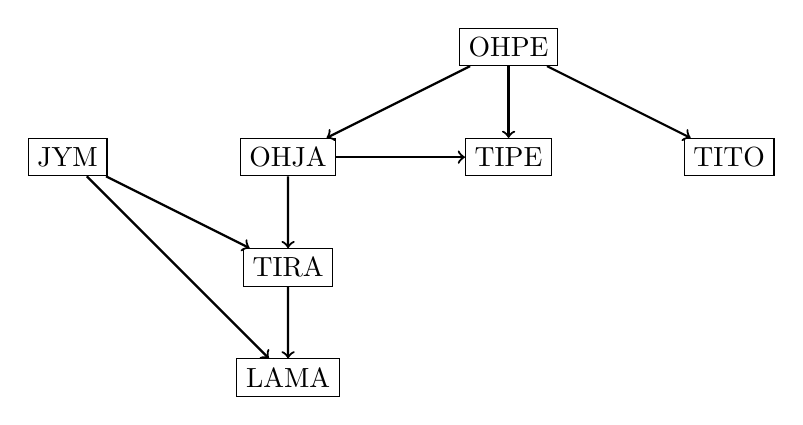
\begin{tikzpicture}[scale=0.7]
\node[draw, rectangle] (1) at (0,0) {OHPE};
\node[draw, rectangle] (2) at (-4,-2) {OHJA};
\node[draw, rectangle] (3) at (4,-2) {TITO};
\node[draw, rectangle] (4) at (0,-2) {TIPE};
\node[draw, rectangle] (5) at (-8,-2) {JYM};
\node[draw, rectangle] (6) at (-4,-4) {TIRA};
\node[draw, rectangle] (7) at (-4,-6) {LAMA};
\path[draw,thick,->] (1) -- (2);
\path[draw,thick,->] (1) -- (3);
\path[draw,thick,->] (1) -- (4);
\path[draw,thick,->] (2) -- (4);
\path[draw,thick,->] (2) -- (6);
\path[draw,thick,->] (5) -- (6);
\path[draw,thick,->] (5) -- (7);
\path[draw,thick,->] (6) -- (7);
\end{tikzpicture}
\end{center}
\caption{Kurssien esitietovaatimukset verkkona.}
\label{fig:kuresi}
\end{figure}

Tällaisen verkon topologinen järjestys kertoo meille
yhden tavan suorittaa kurssit esitietovaatimusten mukaisesti.
Kuva \ref{fig:kurjar} näyttää, kuinka voimme suorittaa
kurssit esimerkkitilanteessamme.
Mahdollinen suoritusjärjestys on siis
OHPE, OHJA, TIPE, TITO, JYM, TIRA, LAMA.

\begin{figure}
\center
\begin{center}
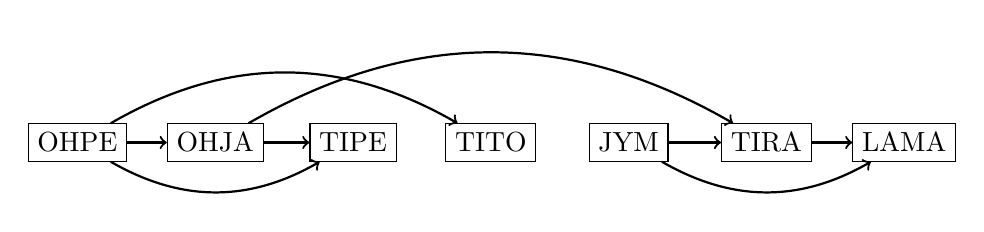
\begin{tikzpicture}[scale=0.7]
\node[draw, rectangle] (1) at (0,0) {OHPE};
\node[draw, rectangle] (2) at (2.5,0) {OHJA};
\node[draw, rectangle] (4) at (5,0) {TIPE};
\node[draw, rectangle] (3) at (7.5,0) {TITO};
\node[draw, rectangle] (5) at (10,0) {JYM};
\node[draw, rectangle] (6) at (12.5,0) {TIRA};
\node[draw, rectangle] (7) at (15,0) {LAMA};
\path[draw,thick,->] (1) -- (2);
\path[draw,thick,->] (1) edge [bend left] (3);
\path[draw,thick,->] (1) edge [bend right] (4);
\path[draw,thick,->] (2) -- (4);
\path[draw,thick,->] (2) edge [bend left] (6);
\path[draw,thick,->] (5) -- (6);
\path[draw,thick,->] (5) edge [bend right] (7);
\path[draw,thick,->] (6) -- (7);
\end{tikzpicture}
\end{center}
\caption{Topologinen järjestys antaa kurssien suoritusjärjestyksen.}
\label{fig:kurjar}
\end{figure}

On selvää, että kurssien ja esitietovaatimusten muodostaman
verkon tulee olla syklitön.
Jos verkossa on sykli, topologista järjestystä ei ole olemassa
eikä meillä ole mitään mahdollisuutta suorittaa kursseja
esitietovaatimusten mukaisesti.

\section{Dynaaminen ohjelmointi}

Kun tiedämme, että suunnattu verkko on syklitön,
voimme ratkaista monia verkko-ongelmia tehokkaasti
dynaamisen ohjelmoinnin avulla.
Esimerkkejä tällaisista ongelmista ovat:

\begin{itemize}
\item Kuinka pitkä on lyhin polku solmusta $a$ solmuun $b$?
\item Kuinka pitkä on pisin polku solmusta $a$ solmuun $b$?
\item Montako erilaista polkua on solmusta $a$ solmuun $b$?
\end{itemize}

Esimerkiksi kuvan \ref{fig:verpol} verkossa on kolme
mahdollista polkua solmusta 1 solmuun 4:
$1 \rightarrow 2 \rightarrow 4$,
$1 \rightarrow 3 \rightarrow 2 \rightarrow 4$ ja
$1 \rightarrow 3 \rightarrow 4$.
Lyhin polun pituus on 2 ja pisin polun pituus on 3.

\begin{figure}
\center
\begin{center}
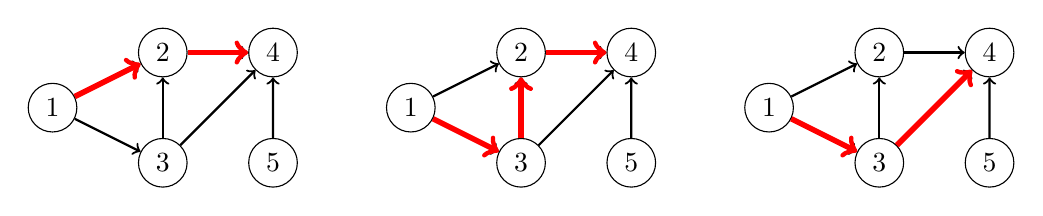
\begin{tikzpicture}[scale=0.7]
\begin{scope}
\node[draw, circle] (1) at (0,-1) {$1$};
\node[draw, circle] (2) at (2,0) {$2$};
\node[draw, circle] (3) at (2,-2) {$3$};
\node[draw, circle] (4) at (4,0) {$4$};
\node[draw, circle] (5) at (4,-2) {$5$};
\path[draw,thick,->] (1) -- (2);
\path[draw,thick,->] (1) -- (3);
\path[draw,thick,->] (3) -- (2);
\path[draw,thick,->] (2) -- (4);
\path[draw,thick,->] (3) -- (4);
\path[draw,thick,->] (5) -- (4);
\path[draw=red,thick,->,line width=2pt] (1) -- (2);
\path[draw=red,thick,->,line width=2pt] (2) -- (4);
\end{scope}
\begin{scope}[xshift=6.5cm]
\node[draw, circle] (1) at (0,-1) {$1$};
\node[draw, circle] (2) at (2,0) {$2$};
\node[draw, circle] (3) at (2,-2) {$3$};
\node[draw, circle] (4) at (4,0) {$4$};
\node[draw, circle] (5) at (4,-2) {$5$};
\path[draw,thick,->] (1) -- (2);
\path[draw,thick,->] (1) -- (3);
\path[draw,thick,->] (3) -- (2);
\path[draw,thick,->] (2) -- (4);
\path[draw,thick,->] (3) -- (4);
\path[draw,thick,->] (5) -- (4);
\path[draw=red,thick,->,line width=2pt] (1) -- (3);
\path[draw=red,thick,->,line width=2pt] (3) -- (2);
\path[draw=red,thick,->,line width=2pt] (2) -- (4);
\end{scope}
\begin{scope}[xshift=13cm]
\node[draw, circle] (1) at (0,-1) {$1$};
\node[draw, circle] (2) at (2,0) {$2$};
\node[draw, circle] (3) at (2,-2) {$3$};
\node[draw, circle] (4) at (4,0) {$4$};
\node[draw, circle] (5) at (4,-2) {$5$};
\path[draw,thick,->] (1) -- (2);
\path[draw,thick,->] (1) -- (3);
\path[draw,thick,->] (3) -- (2);
\path[draw,thick,->] (2) -- (4);
\path[draw,thick,->] (3) -- (4);
\path[draw,thick,->] (5) -- (4);
\path[draw=red,thick,->,line width=2pt] (1) -- (3);
\path[draw=red,thick,->,line width=2pt] (3) -- (4);
\end{scope}
\end{tikzpicture}
\end{center}
\caption{Mahdolliset polut solmusta 1 solmuun 4.}
\label{fig:verpol}
\end{figure}

Osoittautuu, että voimme ratkaista
kaikki yllä mainitut ongelmat
ajassa $O(n+m)$ dynaamisella ohjelmoinnilla,
kun oletamme, että verkko on suunnattu ja syklitön.
Yleisessä verkossa tilanne on toinen:
voimme etsiä lyhimmän polun Dijkstran algoritmilla
ajassa $O(m \log n)$, mutta pisimmän polun etsimiseen
tai polkujen yhteismäärän laskemiseen ei tunneta
mitään tehokasta menetelmää.

\subsection{Polkujen käsittely}

Jotta voimme käyttää dynaamista ohjelmointia,
meidän täytyy määritellä ongelmat rekursiivisesti.
Sopivat funktiot ovat seuraavat:

\begin{itemize}
\item $\texttt{lyhin}(x)$: lyhimmän polun pituus solmusta $a$ solmuun $x$
\item $\texttt{pisin}(x)$: pisimmän polun pituus solmusta $a$ solmuun $x$
\item $\texttt{maara}(x)$: polkujen yhteismäärä solmusta $a$ solmuun $x$
\end{itemize}

Esimerkiksi kuvan \ref{fig:verpol} tilanteessa lähtösolmu on $a=1$
ja funktiot saavat arvot $\texttt{lyhin}(4)=2$,
$\texttt{pisin}(4)=3$ ja $\texttt{maara}(4)=3$.

Funktioiden pohjatapaukset ovat seuraavat:

\begin{align*}
\texttt{lyhin}(a)&=0 \\
\texttt{pisin}(a)&=0 \\
\texttt{maara}(a)&=1
\end{align*}

Tämä tarkoittaa tilannetta, jossa haluamme kulkea solmusta $a$
solmuun $a$. Koska polulla ei ole yhtään kaaria,
sekä lyhimmän että pisimmän polun pituus on 0.
Polkujen määrä on 1, koska ainoa polku on tyhjä polku.

Seuraavaksi määrittelemme yleisen tapauksen solmulle $x$.
Oletamme, että solmuun $x$ pääsee kaarella $k$ solmusta,
joiden tunnukset ovat $u_1,u_2,\dots,u_k$.
Tällöin saamme seuraavat rekursiiviset kaavat:

\begin{align*}
\texttt{lyhin}(x)&=\min(\texttt{lyhin}(u_1),\texttt{lyhin}(u_2),\dots,\texttt{lyhin}(u_k))+1 \\
\texttt{pisin}(x)&=\max(\texttt{pisin}(u_1),\texttt{pisin}(u_2),\dots,\texttt{pisin}(u_k))+1 \\
\texttt{maara}(x)&=\texttt{maara}(u_1)+\texttt{maara}(u_2)+\dots+\texttt{maara}(u_k)
\end{align*}

Kun haluamme muodostaa lyhimmän polun solmusta $a$ solmuun $x$,
meidän tulee valita edellinen solmu niin,
että siihen on lyhin matka solmusta $a$.
Niinpä valitsemme minimin edellisistä arvoista
ja lisäämme siihen yhden.
Vastaavasti kun haluamme muodostaa pisimmän polun,
valitsemme maksimin edellisistä arvoista.
Kun taas haluamme laskea polkujen yhteismäärän,
laskemme yhteen kaikki solmuun johtavat polut.

Tarkastellaan esimerkkinä kuvan \ref{fig:verpol} verkkoa,
jossa tutkimme polkuja solmusta 1 solmuun 4.
Kun haluamme laskea funktioiden arvot solmulle 4,
otamme huomioon kaaret
$2 \rightarrow 4$, $3 \rightarrow 4$ ja $5 \rightarrow 4$,
joita kulkemalla pääsee muista solmuista solmuun 4.
Oletamme, että olemme laskeneet aiemmin funktioiden
arvot solmuille 2, 3 ja 5.

Nyt esimerkiksi lyhin polku solmusta 1 solmuun 4 on pituudeltaan
\[ \texttt{lyhin}(4)=\min(\texttt{lyhin}(2),\texttt{lyhin}(3),\texttt{lyhin}(5))+1.\]
Aiemmat arvot ovat $\texttt{lyhin}(2)=1$, $\texttt{lyhin}(3)=2$ ja $\texttt{lyhin}(5)=\infty$.
Valitsemme näistä pienimmän, eli tulemme solmuun 4 solmusta 2.
Tämä tuottaa polun, jonka pituus on $\texttt{lyhin}(2)+1=2$.

Huomaa, että jos solmuun $x$ ei tule kaarta mistään solmusta,
oletamme, että $\texttt{lyhin}(x)=\infty$ ja $\texttt{pisin}(x)=-\infty$.
Tämä on luonteva tulkinta, kun laskemme minimin tai maksimin
tyhjälle joukolle.
Tämän ansiosta emme koskaan muodosta polkua,
joka ei ala solmusta $a$.

Koska tiedämme, että verkko on syklitön,
voimme laskea rekursiivisten funktioiden arvot
tehokkaasti dynaamisella ohjelmoinnilla.
Oleellista on, että emme voi joutua koskaan silmukkaan
laskiessamme arvoja.
Tällä tavalla saamme kuhunkin ongelmaan ratkaisun, joka
vie aikaa $O(n+m)$.

\subsection{Ongelmat verkkoina}

Itse asiassa \emph{minkä tahansa} dynaamisen ohjelmoinnin ratkaisun voi
esittää suunnattuna syklittömänä verkkona.
Tällöin jokainen verkon solmu vastaa yhtä laskettavaa funktion arvoa,
ja kaaret näyttävät, miten funktion arvot riippuvat toisistaan.

Tarkastellaan esimerkkinä tuttua tehtävää,
jossa haluamme muodostaa rahasumman annetuista kolikoista.
Esimerkiksi jos kolikot ovat $\{1,3,4\}$ ja rahasumma on 6,
ratkaisut ovat seuraavat:

\begin{multicols}{2}
\begin{itemize}
\item $4+1+1$
\item $1+4+1$
\item $1+1+4$
\item $3+3$
\item $3+1+1+1$
\item $1+3+1+1$
\item $1+1+3+1$
\item $1+1+1+3$
\item $1+1+1+1+1+1$
\end{itemize}
\end{multicols}

\begin{figure}
\center
\begin{center}
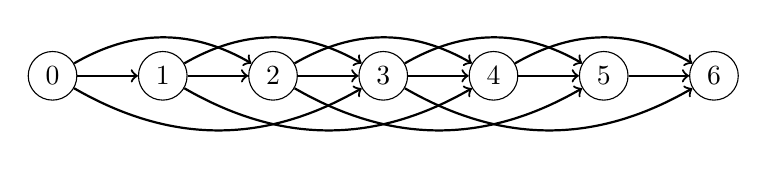
\begin{tikzpicture}[scale=0.7]
\node[draw, circle] (0) at (0,0) {$0$};
\node[draw, circle] (1) at (2,0) {$1$};
\node[draw, circle] (2) at (4,0) {$2$};
\node[draw, circle] (3) at (6,0) {$3$};
\node[draw, circle] (4) at (8,0) {$4$};
\node[draw, circle] (5) at (10,0) {$5$};
\node[draw, circle] (6) at (12,0) {$6$};
\path[draw,thick,->] (0) -- (1);
\path[draw,thick,->] (1) -- (2);
\path[draw,thick,->] (2) -- (3);
\path[draw,thick,->] (3) -- (4);
\path[draw,thick,->] (4) -- (5);
\path[draw,thick,->] (5) -- (6);
\path[draw,thick,->] (0) edge [bend left] (2);
\path[draw,thick,->] (1) edge [bend left] (3);
\path[draw,thick,->] (2) edge [bend left] (4);
\path[draw,thick,->] (3) edge [bend left] (5);
\path[draw,thick,->] (4) edge [bend left] (6);
\path[draw,thick,->] (0) edge [bend right] (3);
\path[draw,thick,->] (1) edge [bend right] (4);
\path[draw,thick,->] (2) edge [bend right] (5);
\path[draw,thick,->] (3) edge [bend right] (6);
\end{tikzpicture}
\end{center}
\caption{Kolikkotehtävä esitettynä verkkona.}
\label{fig:verkol}
\end{figure}

Voimme esittää tämän tehtävän verkkona niin,
että solmut ovat rahasummia ja kaaret kertovat,
kuinka voimme valita kolikkoja.
Esimerkiksi kuva \ref{fig:verkol} näyttää verkon,
joka vastaa yllä olevaa tapausta.
Tässä verkossa lyhin polku solmusta 0 solmuun 6
($0 \rightarrow 3 \rightarrow 6$)
vastaa ratkaisua $3+3$, jossa kolikoiden määrä on pienin,
ja polkujen yhteismäärä solmusta 0 solmuun 6 on 9,
joka on sama kuin kaikkien ratkaisuiden määrä.

Olemme saaneet siis uuden tavan luonnehtia dynaamista ohjelmointia:
voimme käyttää dynaamista ohjelmointia,
jos pystymme esittämään ongelman suunnattuna syklittömänä verkkona.

\section{Vahvasti yhtenäisyys}

Jos suunnatussa verkossa on sykli,
emme voi muodostaa sille topologista järjestystä
emmekä käyttää dynaamista ohjelmointia.
Mikä neuvoksi, jos kuitenkin haluaisimme tehdä näin?

Joskus voimme ratkaista asian etsimällä
verkon vahvasti yhtenäiset komponentit.
Vahvasti yhtenäinen komponentti on joukko verkon solmuja,
jossa pätee, että mistä tahansa solmusta on polku
mihin tahansa solmuun.
Kun esitämme jokaisen vahvasti yhtenäisen komponentin
yhtenä solmuna, saamme esille verkon syvärakenteen,
joka on aina syklitön verkko.

\begin{figure}
\center
\begin{center}
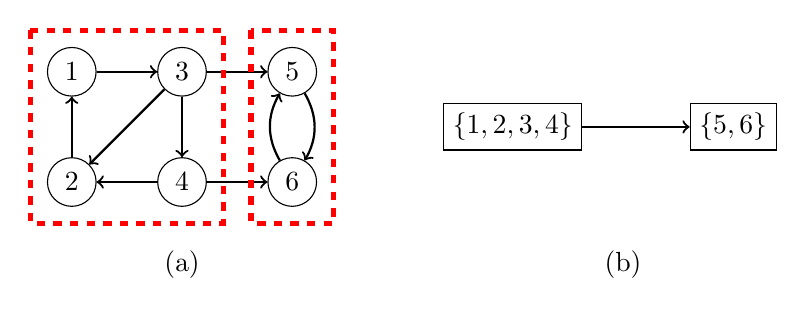
\begin{tikzpicture}[scale=0.7]
\begin{scope}
\node[draw, circle] (1) at (0,0) {$1$};
\node[draw, circle] (2) at (0,-2) {$2$};
\node[draw, circle] (3) at (2,0) {$3$};
\node[draw, circle] (4) at (2,-2) {$4$};
\node[draw, circle] (5) at (4,0) {$5$};
\node[draw, circle] (6) at (4,-2) {$6$};

\path[draw,thick,->] (1) -- (3);
\path[draw,thick,->] (3) -- (4);
\path[draw,thick,->] (4) -- (2);
\path[draw,thick,->] (2) -- (1);
\path[draw,thick,->] (3) -- (2);

\path[draw,thick,->] (5) edge [bend left] (6);
\path[draw,thick,->] (6) edge [bend left] (5);

\path[draw,thick,->] (3) -- (5);
\path[draw,thick,->] (4) -- (6);

\draw[red,dashed,thick,line width=2pt] (-0.75,0.75) rectangle (2.75,-2.75);
\draw[red,dashed,thick,line width=2pt] (3.25,0.75) rectangle (4.75,-2.75);

\node at (2,-3.5) {(a)};
\end{scope}
\begin{scope}[xshift=8cm,yshift=-1cm]
\node[draw,rectangle] (1) at (0,0) {$\{1,2,3,4\}$};
\node[draw,rectangle] (2) at (4,0) {$\{5,6\}$};
\path[draw,thick,->] (1) -- (2);
\node at (2,-2.5) {(b)};
\end{scope}
\end{tikzpicture}
\end{center}
\caption{(a) Verkon vahvasti yhtenäiset komponentit.
(b) Komponenttiverkko, joka kuvaa verkon syvärakenteen.}
\label{fig:vahkom}
\end{figure}

Kuvassa \ref{fig:vahkom} on esimerkkinä verkko, joka muodostuu
kahdesta vahvasti yhtenäisestä komponentista.
Ensimmäinen komponentti on $\{1,2,3,4\}$
ja toinen komponentti on $\{5,6\}$.
Komponenteista muodostuu syklitön komponenttiverkko,
jossa on kaari solmusta $\{1,2,3,4\}$ solmuun $\{5,6\}$.

Seuraavaksi tutustumme Kosarajun algoritmiin,
jonka avulla pystymme etsimään tehokkaasti suunnatun
verkon vahvasti yhtenäiset komponentit ja niitä
vastaavan komponenttiverkon.

\subsection{Kosarajun algoritmi}

Kosarajun algoritmi muodostuu kahdesta verkon läpikäynnistä.
Ensimmäinen läpikäynti muistuttaa topologisen järjestyksen
muodostamista ja tuottaa listan solmuista.
Toinen läpikäynti muodostaa vahvasti yhtenäiset komponentit
ensimmäisen läpikäynnin tuottaman listan avulla.

Algoritmin ensimmäinen läpikäynti aloittaa vuorollaan
syvyyshaun jokaisesta solmusta, jota ei ole vielä käsitelty.
Jokaisessa solmussa käymme ensin läpi kaikki
solmusta lähtevät kaaret ja lisäämme tämän jälkeen solmun listalle.
Toimimme siis kuten topologisen järjestyksen muodostamisessa,
mutta emme välitä, jos tulemme uudestaan samaan solmuun.

Algoritmin toisen läpikäynnin alussa
käännämme jokaisen verkon kaaren suunnan.
Tämän jälkeen käsittelemme ensimmäisen läpikäynnin tuottaman
solmujen listan kääntei\-sessä järjestyksessä.
Jokaisen solmun kohdalla muodostamme uuden vahvasti yhtenäisen
komponentin, jossa on kaikki vielä käsittelemät\-tömät solmut,
joihin pääsemme solmusta.

\begin{figure}
\center
\begin{center}
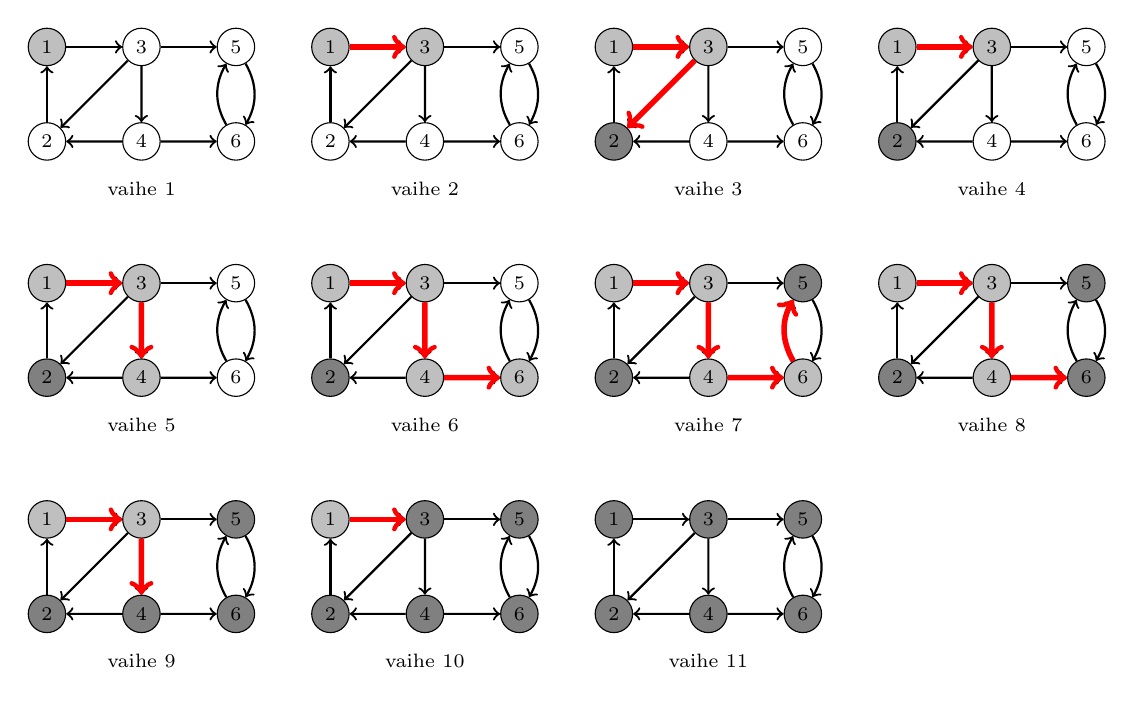
\begin{tikzpicture}[scale=0.6]
\scriptsize
\newcommand\verkko[7]{
\node[draw, circle, fill=#2] (1) at (0,0) {$1$};
\node[draw, circle, fill=#3] (2) at (0,-2) {$2$};
\node[draw, circle, fill=#4] (3) at (2,0) {$3$};
\node[draw, circle, fill=#5] (4) at (2,-2) {$4$};
\node[draw, circle, fill=#6] (5) at (4,0) {$5$};
\node[draw, circle, fill=#7] (6) at (4,-2) {$6$};

\path[draw,thick,->] (1) -- (3);
\path[draw,thick,->] (3) -- (4);
\path[draw,thick,->] (4) -- (2);
\path[draw,thick,->] (2) -- (1);
\path[draw,thick,->] (3) -- (2);
\path[draw,thick,->] (5) edge [bend left] (6);
\path[draw,thick,->] (6) edge [bend left] (5);
\path[draw,thick,->] (3) -- (5);
\path[draw,thick,->] (4) -- (6);

\node at (2,-3) {vaihe #1};
}
\begin{scope}
\verkko{1}{lightgray}{white}{white}{white}{white}{white}
\end{scope}
\begin{scope}[xshift=6cm]
\verkko{2}{lightgray}{white}{lightgray}{white}{white}{white}
\path[draw=red,thick,->,line width=2pt] (1) -- (3);
\end{scope}
\begin{scope}[xshift=12cm]
\verkko{3}{lightgray}{gray}{lightgray}{white}{white}{white}
\path[draw=red,thick,->,line width=2pt] (1) -- (3);
\path[draw=red,thick,->,line width=2pt] (3) -- (2);
\end{scope}
\begin{scope}[xshift=18cm]
\verkko{4}{lightgray}{gray}{lightgray}{white}{white}{white}
\path[draw=red,thick,->,line width=2pt] (1) -- (3);
\end{scope}
\begin{scope}[yshift=-5cm]
\verkko{5}{lightgray}{gray}{lightgray}{lightgray}{white}{white}
\path[draw=red,thick,->,line width=2pt] (1) -- (3);
\path[draw=red,thick,->,line width=2pt] (3) -- (4);
\end{scope}
\begin{scope}[yshift=-5cm,xshift=6cm]
\verkko{6}{lightgray}{gray}{lightgray}{lightgray}{white}{lightgray}
\path[draw=red,thick,->,line width=2pt] (1) -- (3);
\path[draw=red,thick,->,line width=2pt] (3) -- (4);
\path[draw=red,thick,->,line width=2pt] (4) -- (6);
\end{scope}
\begin{scope}[yshift=-5cm,xshift=12cm]
\verkko{7}{lightgray}{gray}{lightgray}{lightgray}{gray}{lightgray}
\path[draw=red,thick,->,line width=2pt] (1) -- (3);
\path[draw=red,thick,->,line width=2pt] (3) -- (4);
\path[draw=red,thick,->,line width=2pt] (4) -- (6);
\path[draw=red,thick,->,line width=2pt] (6) edge [bend left] (5);
\end{scope}
\begin{scope}[yshift=-5cm,xshift=18cm]
\verkko{8}{lightgray}{gray}{lightgray}{lightgray}{gray}{gray}
\path[draw=red,thick,->,line width=2pt] (1) -- (3);
\path[draw=red,thick,->,line width=2pt] (3) -- (4);
\path[draw=red,thick,->,line width=2pt] (4) -- (6);
\end{scope}
\begin{scope}[yshift=-10cm]
\verkko{9}{lightgray}{gray}{lightgray}{gray}{gray}{gray}
\path[draw=red,thick,->,line width=2pt] (1) -- (3);
\path[draw=red,thick,->,line width=2pt] (3) -- (4);
\end{scope}
\begin{scope}[yshift=-10cm,xshift=6cm]
\verkko{10}{lightgray}{gray}{gray}{gray}{gray}{gray}
\path[draw=red,thick,->,line width=2pt] (1) -- (3);
\end{scope}
\begin{scope}[yshift=-10cm,xshift=12cm]
\verkko{11}{gray}{gray}{gray}{gray}{gray}{gray}
\end{scope}
\end{tikzpicture}
\end{center}
\caption{Kosarajun algoritmin ensimmäinen läpikäynti.}
\label{fig:koseka}
\end{figure}

Tarkastelemme seuraavaksi, kuinka Kosarajun algoritmi
toimii esimerkkiverkossamme.
Kuva \ref{fig:koseka} näyttää ensimmäisen läpikäynnin,
joka muodostaa solmuista listan $[2,5,6,4,3,1]$.
Tämän jälkeen käännämme kaikki verkon kaaret ja
käsittelemme solmut järjestyksessä $[1,3,4,6,5,2]$.
Kuva \ref{fig:kostok} näyttää toisen läpikäynnin.
Vahvasti yhtenäiset komponentit syntyvät
solmuista 1 ja 6 alkaen.
Kaarten kääntämisen ansiosta
solmusta 1 alkava
vahvasti yhtenäinen komponentti ei ''vuoda''
solmujen 5 ja 6 alueelle.

\begin{figure}
\center
\begin{center}
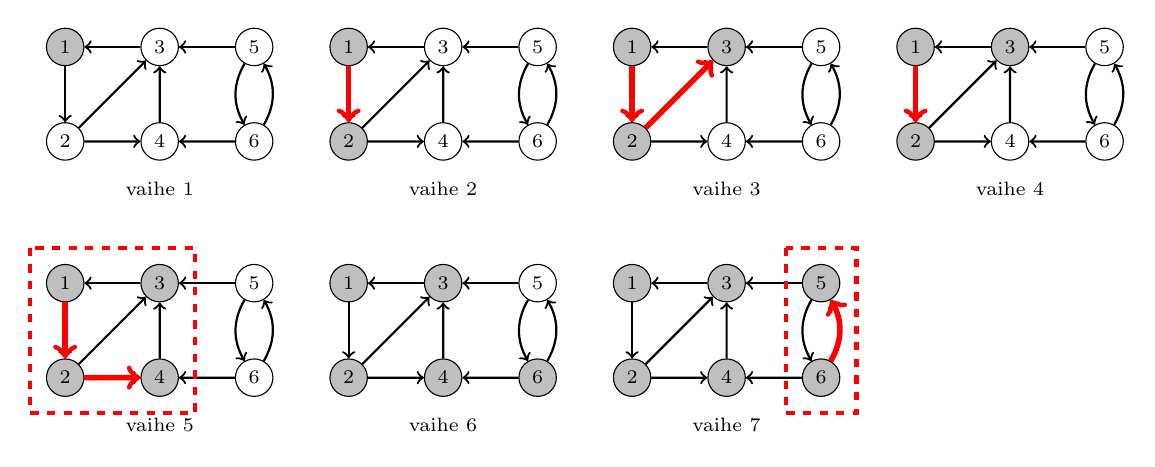
\begin{tikzpicture}[scale=0.6]
\scriptsize
\newcommand\verkko[7]{
\node[draw, circle, fill=#2] (1) at (0,0) {$1$};
\node[draw, circle, fill=#3] (2) at (0,-2) {$2$};
\node[draw, circle, fill=#4] (3) at (2,0) {$3$};
\node[draw, circle, fill=#5] (4) at (2,-2) {$4$};
\node[draw, circle, fill=#6] (5) at (4,0) {$5$};
\node[draw, circle, fill=#7] (6) at (4,-2) {$6$};

\path[draw,thick,<-] (1) -- (3);
\path[draw,thick,<-] (3) -- (4);
\path[draw,thick,<-] (4) -- (2);
\path[draw,thick,<-] (2) -- (1);
\path[draw,thick,<-] (3) -- (2);
\path[draw,thick,<-] (5) edge [bend left] (6);
\path[draw,thick,<-] (6) edge [bend left] (5);
\path[draw,thick,<-] (3) -- (5);
\path[draw,thick,<-] (4) -- (6);

\node at (2,-3) {vaihe #1};
}
\begin{scope}
\verkko{1}{lightgray}{white}{white}{white}{white}{white}
\end{scope}
\begin{scope}[xshift=6cm]
\verkko{2}{lightgray}{lightgray}{white}{white}{white}{white}
\path[draw=red,thick,->,line width=2pt] (1) -- (2);
\end{scope}
\begin{scope}[xshift=12cm]
\verkko{3}{lightgray}{lightgray}{lightgray}{white}{white}{white}
\path[draw=red,thick,->,line width=2pt] (1) -- (2);
\path[draw=red,thick,->,line width=2pt] (2) -- (3);
\end{scope}
\begin{scope}[xshift=18cm]
\verkko{4}{lightgray}{lightgray}{lightgray}{white}{white}{white}
\path[draw=red,thick,->,line width=2pt] (1) -- (2);
\end{scope}
\begin{scope}[yshift=-5cm]
\verkko{5}{lightgray}{lightgray}{lightgray}{lightgray}{white}{white}
\path[draw=red,thick,->,line width=2pt] (1) -- (2);
\path[draw=red,thick,->,line width=2pt] (2) -- (4);
\draw[red,dashed,thick,line width=1.5pt] (-0.75,0.75) rectangle (2.75,-2.75);
\end{scope}
\begin{scope}[yshift=-5cm,xshift=6cm]
\verkko{6}{lightgray}{lightgray}{lightgray}{lightgray}{white}{lightgray}
\end{scope}
\begin{scope}[yshift=-5cm,xshift=12cm]
\verkko{7}{lightgray}{lightgray}{lightgray}{lightgray}{lightgray}{lightgray}
\path[draw=red,thick,<-,line width=2pt] (5) edge [bend left] (6);
\draw[red,dashed,thick,line width=1.5pt] (3.25,0.75) rectangle (4.75,-2.75);
\end{scope}
\end{tikzpicture}
\end{center}
\caption{Kosarajun algoritmin toinen läpikäynti.}
\label{fig:kostok}
\end{figure}

Koska algoritmi muodostuu kahdesta verkon läpikäynnistä,
sen aikavaativuus on $O(n+m)$.

\subsection{Miksi algoritmi toimii?}

Keskeinen kysymys Kosarajun algoritmiin liittyen on,
miten voimme olla varmoja, että saamme verkon toisessa läpikäynnissä
muodostettua vahvasti yhtenäisiä komponentteja,
joihin ei tule ylimääräisiä solmuja?

Voimme tarkastella asiaa muodostettavana olevan syklittömän
komponenttiverkon näkökulmasta.
Jos meillä on komponentti $A$, josta pääsee kaarella
komponenttiin $B$, 
algoritmin ensimmäinen läpikäynti takaa,
jokin $A$:n solmu lisätään listalle kaikkien $B$:n
solmujen jälkeen.
Kun sitten käymme läpi listan käänteisessä järjestyksessä,
jokin $A$:n solmu tulee vastaan ennen kaikkia $B$:n
solmuja.
Niinpä alamme rakentaa komponenttia $A$,
emmekä mene komponentin $B$ puolelle,
koska verkon kaaret on käännetty.

Vastaavasti jos meillä on komponentti $A$,
johon pääsee komponentista $B$,
muodostamme komponentin $B$ ennen komponenttia $A$.
Niinpä kun käänteisessä verkossa
komponentista $A$ on kaari komponenttiin $B$,
tämä ei haittaa, koska olemme jo muodostaneet
komponentin $B$ eikä komponenttiin $A$ tule ylimääräisiä solmuja
komponentista $B$.

\section{Esimerkki: Luolapeli}

Olemme pelissä luolastossa, joka muodostuu luolista ja niitä yhdistävistä
käytävistä. Jokainen käytävä on yksisuuntainen.
Jokaisessa luolassa on yksi aarre, jonka voimme ottaa mukaamme,
jos kuljemme luolan kautta.

Peli alkaa luolasta $a$ ja päättyy luolaan $b$.
Montako aarretta voimme saada, jos valitsemme parhaan
mahdollisen reitin?

\subsubsection{Ratkaisu}

Voimme mallintaa tilanteen verkkona, jonka solmut ovat luolia ja
kaaret ovat käytäviä. Haluamme löytää reitin solmusta $a$ solmuun $b$
niin, että kuljemme mahdollisimman monen solmun kautta.

\begin{figure}
\center
\begin{center}
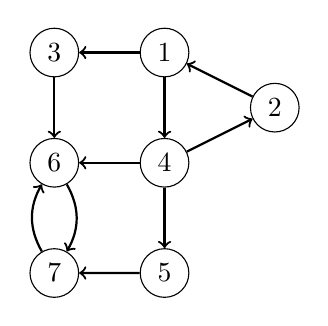
\begin{tikzpicture}[scale=0.7]
\node[draw, circle] (1) at (0,0) {$1$};
\node[draw, circle] (2) at (2,-1) {$2$};
\node[draw, circle] (3) at (-2,0) {$3$};
\node[draw, circle] (4) at (0,-2) {$4$};
\node[draw, circle] (5) at (0,-4) {$5$};
\node[draw, circle] (6) at (-2,-2) {$6$};
\node[draw, circle] (7) at (-2,-4) {$7$};

\path[draw,thick,->] (1) -- (4);
\path[draw,thick,->] (4) -- (2);
\path[draw,thick,->] (2) -- (1);
\path[draw,thick,->] (4) -- (6);
\path[draw,thick,->] (1) -- (3);
\path[draw,thick,->] (3) -- (6);
\path[draw,thick,->] (6) edge [bend left] (7);
\path[draw,thick,->] (7) edge [bend left] (6);
\path[draw,thick,->] (4) -- (5);
\path[draw,thick,->] (5) -- (7);
\end{tikzpicture}
\end{center}
\caption{Luolasto, jossa on 7 luolaa ja 10 käytävää.
Haluamme kulkea luolasta 1 luolaan 7 keräten mahdollisimman paljon aarteita.}
\label{fig:luopel}
\end{figure}

Esimerkiksi kuva \ref{fig:luopel} näyttää verkkona luolaston, joka muodostuu
7 luolasta ja 10 käytävästä.
Oletetaan, että haluamme liikkua luolasta 1 luolaan 7
keräten mahdollisimman paljon aarteita.
Tällöin yksi mahdollinen reitti on
$1 \rightarrow 4 \rightarrow 2 \rightarrow 1 \rightarrow 3 \rightarrow 6 \rightarrow 7$,
jonka avulla saamme kaikki aarteet paitsi luolassa 5 olevan aarteen.
Ei ole olemassa reittiä, jota seuraamalla saisimme kaikki luolaston aarteet.

\begin{figure}
\center
\begin{center}
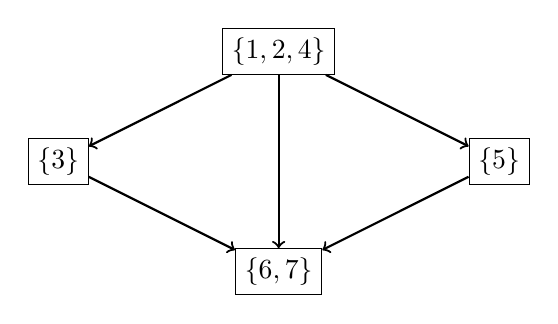
\begin{tikzpicture}[scale=0.7]
\node[draw, rectangle] (1) at (0,0) {$\{1,2,4\}$};
\node[draw, rectangle] (2) at (-4,-2) {$\{3\}$};
\node[draw, rectangle] (3) at (4,-2) {$\{5\}$};
\node[draw, rectangle] (4) at (0,-4) {$\{6,7\}$};

\path[draw,thick,->] (1) -- (2);
\path[draw,thick,->] (1) -- (3);
\path[draw,thick,->] (1) -- (4);
\path[draw,thick,->] (2) -- (4);
\path[draw,thick,->] (3) -- (4);
\end{tikzpicture}
\end{center}
\caption{Luolaston vahvasti yhtenäiset komponentit.}
\label{fig:luovah}
\end{figure}

Voimme ratkaista ongelman tehokkaasti määrittämällä ensin verkon
vahvasti yhtenäiset komponentit.
Tämän jälkeen meidän riittää löytää polku alkusolmun komponentista
loppusolmun komponenttiin niin, että komponenttien kokojen summa
on suurin mahdollinen.
Koska verkko on syklitön, tämä onnistuu dynaamisella ohjelmoinnilla.

Kuva \ref{fig:luovah} näyttää vahvasti yhtenäiset komponentit
esimerkkiverkossamme.
Tästä esityksestä näemme suoraan, että optimaalisia reittejä on kaksi:
voimme kulkea joko luolan 3 tai luolan 5 kautta.
\chapter{Komponentit ja virittävät puut}

Tähän mennessä olemme tarkastelleet verkkoja,
joiden rakenne säilyy samana koko algoritmin ajan.
Mitä tapahtuu sitten, jos verkkoon tuleekin \emph{muutoksia},
kuten lisäämme verkkoon uusia kaaria?

Tutustumme tässä luvussa union-find-rakenteeseen,
joka on hyödyl\-linen työkalu verkkojen käsittelyssä.
Rakenteen avulla voimme pitää kirjaa verkon yhtenäisistä
komponenteista ja päivittää rakennetta tehokkaasti,
kun lisäämme verkkoon kaaria.
Voimme esimerkiksi tarkkailla, montako yhte\-näistä
komponenttia verkossa on milläkin hetkellä.

Käsittelemme myös pienimmän virittävän puun ongelmaa,
jossa haluamme kytkeä verkon solmut toisiinsa kaaria käyttäen niin,
että kaarten yhteispaino on pienin.
Voimme ratkaista ongelman tehokkaasti Kruskalin algoritmilla,
joka perustuu union-find-rakenteeseen,
tai Primin algoritmilla, joka muistuttaa Dijkstran algoritmia.

\section{Union-find-rakenne}

Union-find-rakenne on tietorakenne, joka
pitää yllä kokoelmaa alkioiden joukkoja ja tarjoaa
seuraavat tehokkaat operaatiot:

\begin{itemize}
\item tarkasta, ovatko kaksi alkiota samassa joukossa
\item yhdistä kaksi joukkoa samaksi joukoksi
\end{itemize}

Oletamme, että alkiot ovat $1,2,\dots,n$,
ja jokainen alkio kuuluu tarkalleen yhteen joukkoon.
Esimerkiksi kun $n=8$, joukot voivat olla vaikkapa
$A=\{1,4\}$, $B=\{2,5,6\}$ ja $C=\{3,7,8\}$.
Kun yhdistämme sitten joukot $A$ ja $B$,
niistä syntyy joukko $\{1,2,4,5,6\}$.
Ennen yhdistämistä alkiot $1$ ja $2$ olivat eri joukoissa,
mutta yhdistämisen jälkeen ne ovat samassa joukossa.

\subsection{Rakenteen toteutus}

Toteutamme union-find-rakenteen niin,
että jokaisessa joukossa
yksi alkioista on joukon \emph{edustaja}.
Kutakin joukkoa vastaa puu,
jonka juurena on joukon edustaja ja
muut alkiot viittaavat edustajaan yhden tai useamman kaaren kautta.
Kun haluamme tarkastaa, ovatko kaksi alkiota samassa joukossa,
selvitämme niiden edustajat ja vertaamme niitä toisiinsa.

Kuvassa \ref{fig:unifin} on esimerkkinä union-find-rakenne,
joka vastaa joukkoja $A=\{1,4\}$, $B=\{2,5,6\}$ ja $C=\{3,7,8\}$.
Tässä tapauksessa joukkojen edustajat ovat 1, 5 ja 3.
Esimerkiksi jos haluamme tarkastaa, ovatko alkiot 2 ja 6
samassa joukossa, selvitämme ensin alkioiden edustajat
kulkemalla polkuja $2 \rightarrow 5$ ja $6 \rightarrow 5$.
Kummankin alkion edustaja on $5$, joten toteamme,
että alkiot ovat samassa joukossa.

\begin{figure}
\center
\begin{center}
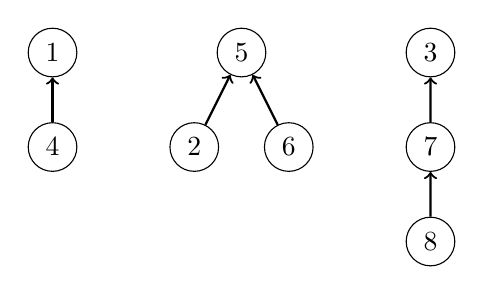
\begin{tikzpicture}[scale=0.6]
\node[draw, circle] (1) at (0,0) {$1$};
\node[draw, circle] (4) at (0,-2) {$4$};

\node[draw, circle] (2) at (3,-2) {$2$};
\node[draw, circle] (5) at (4,0) {$5$};
\node[draw, circle] (6) at (5,-2) {$6$};

\node[draw, circle] (3) at (8,0) {$3$};
\node[draw, circle] (7) at (8,-2) {$7$};
\node[draw, circle] (8) at (8,-4) {$8$};

\path[draw,thick,->] (4) -- (1);
\path[draw,thick,->] (2) -- (5);
\path[draw,thick,->] (6) -- (5);
\path[draw,thick,->] (7) -- (3);
\path[draw,thick,->] (8) -- (7);
\end{tikzpicture}
\end{center}
\caption{Union-find-rakenne joukoille $\{1,4\}$, $\{2,5,6\}$ ja $\{3,7,8\}$.}
\label{fig:unifin}
\end{figure}

Jotta saamme toteutettua union-find-rakenteen,
pidämme yllä jokaiselle alkiolle $x$ arvoa $\texttt{vanhempi}[x]$,
joka kertoo seuraavan alkion ylempänä puussa.
Kuitenkin jos $x$ on joukon edustaja,
$\texttt{vanhempi}[x]=x$.
Esimerkiksi kuvassa \ref{fig:unifin}
$\texttt{vanhempi}[2]=5$ ja $\texttt{vanhempi}[5]=5$.
Tämän ansiosta pystymme selvittämään alkion $x$
edustajan seuraavasti:                                                          

\begin{code}
function edustaja(x)
    while x != vanhempi[x]
        x = vanhempi[x]
    return x
\end{code}

Tämän jälkeen voimme tarkastaa seuraavalla operaatiolla,
ovatko alkiot $a$ ja $b$ samassa joukossa.
Alkiot ovat samassa joukossa täsmälleen silloin, kun niillä
on sama edustaja:

\begin{code}
function sama(a,b)
    return edustaja(a) == edustaja(b)
\end{code}

Haluamme toteuttaa vielä operaation, jolla voimme
yhdistää kaksi joukkoa toisiinsa.
Tämän operaation toteutus ratkaisee, kuinka tehokas rakenteemme on.
Alkion edustajan etsiminen vie aikaa $O(k)$,
missä $k$ on polun pituus,
joten haluamme toteuttaa yhdistämiset niin,
että puussa on vain lyhyitä polkuja.
Saavutamme tämän tavoitteen yhdistämällä kaksi joukkoa
aina asettamalla \emph{pienemmän} joukon
edustajan osoittamaan \emph{suuremman} joukon edustajaan.
Jos joukot ovat yhtä suuria, voimme toteuttaa yhdistämisen kummin päin vain.

\begin{figure}
\center
\begin{center}
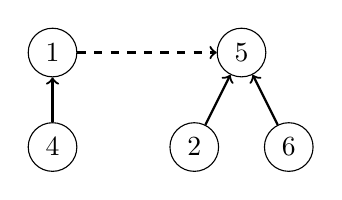
\begin{tikzpicture}[scale=0.6]
\node[draw, circle] (1) at (0,0) {$1$};
\node[draw, circle] (2) at (0,-2) {$4$};
\node[draw, circle] (3) at (4,0) {$5$};
\node[draw, circle] (4) at (3,-2) {$2$};
\node[draw, circle] (5) at (5,-2) {$6$};
\path[draw,thick,->] (2) -- (1);
\path[draw,thick,->] (4) -- (3);
\path[draw,thick,->] (5) -- (3);
\path[draw,thick,->,dashed] (1) -- (3);
\end{tikzpicture}
\end{center}
\caption{Tehokas yhdistäminen. Alkion $1$ joukon koko on 2
ja alkion $5$ joukon koko on 3,
joten yhdistämme alkion 1 alkioon 5.}
\label{fig:tehyhd}
\end{figure}

Kuva \ref{fig:tehyhd} näyttää, mitä tapahtuu, kun yhdistämme joukot
$A=\{1,4\}$ ja $B=\{2,5,6\}$.
Joukon $A$ edustaja on $1$ ja siinä on kaksi alkiota,
kun taas joukon $B$ edustaja on $5$ ja siinä on kolme alkiota.
Koska joukko $A$ on pienempi, asetamme joukon $A$
edustajan osoittamaan joukon $B$ edustajaan.
Tämän jälkeen kaikki alkiot kuuluvat samaan joukkoon ja
alkio $5$ on tästä lähtien koko joukon edustaja.

Nyt olemme valmiita toteuttamaan operaation,
joka yhdistää toisiinsa joukot, joissa on alkiot $a$ ja $b$.
Oletamme, että alkiot ovat eri joukoissa ennen yhdistämistä.
Jotta voimme toteuttaa yhdistämisen tehokkaasti,
meidän täytyy myös pitää kirjaa kunkin joukon koosta.
Seuraavassa toteutuksessa $\texttt{koko}[x]$ kertoo,
montako alkiota alkion $x$ edustama joukko sisältää.

\begin{code}
function yhdista(a,b)
    a = edustaja(a)
    b = edustaja(b)
    if koko[a] < koko[b]
        swap(a,b)
    vanhempi[b] = a
    koko[a] += koko[b]
\end{code}

Kun toteutamme yhdistämiset tällä tavalla, jokainen
puussa esiintyvä polku sisäl\-tää vain $O(\log n)$ alkiota.
Tämä johtuu siitä, että aina kun kuljemme polkua
askeleen ylöspäin alkiosta $a$ alkioon $b$,
$\texttt{koko}[b] \ge 2 \cdot \texttt{koko}[a]$ eli
edustajaa vastaavan joukon koko ainakin \emph{kaksinkertaistuu}.
Koska joukossa on enintään $n$ alkiota,
kuljemme siis yhteensä enintään $O(\log n)$ askelta.
Niinpä kaikki union-find-rakenteen operaatiot
toimivat ajassa $O(\log n)$.

\subsection{Esimerkki: Kaupungit}

Bittimaassa on $n$ kaupunkia, joiden välillä ei ole vielä yhtään tietä.
Sitten teitä aletaan rakentaa yksi kerrallaan, yhteensä $m$ tietä.
Jokainen tie yhdistää kaksi kaupunkia toisiinsa.
Minkä tien rakentamisen jälkeen kaikki kaupungit ovat ensimmäistä
kertaa yhteydessä toisiinsa?

\begin{figure}
\center
\begin{center}
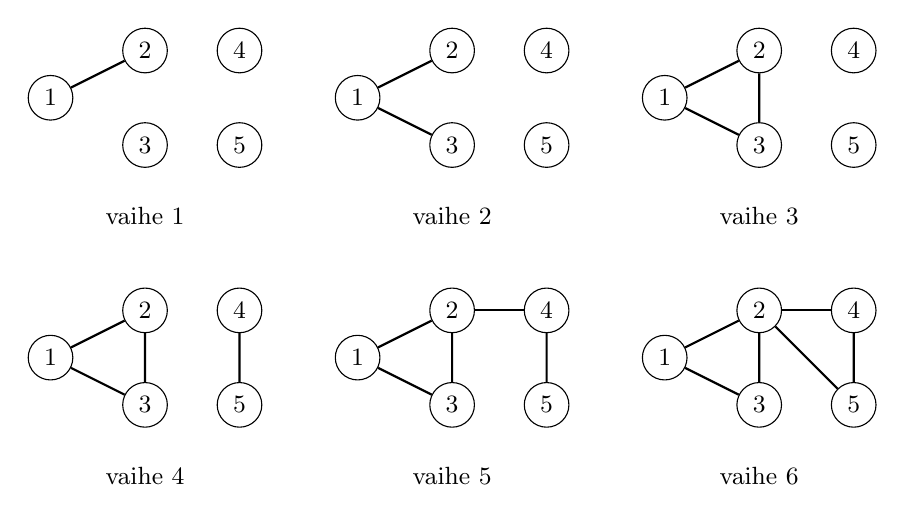
\begin{tikzpicture}[scale=0.6,label distance=-1.5mm]
\small
\newcommand\verkko[1]{
\node[draw, circle] (1) at (0,-1) {$1$};
\node[draw, circle] (2) at (2,0) {$2$};
\node[draw, circle] (3) at (2,-2) {$3$};
\node[draw, circle] (4) at (4,0) {$4$};
\node[draw, circle] (5) at (4,-2) {$5$};
\node at (2,-3.5) {vaihe #1};
}
\begin{scope}
\verkko{1}
\path[draw,thick,-] (1) -- (2);
\end{scope}
\begin{scope}[xshift=6.5cm]
\verkko{2}
\path[draw,thick,-] (1) -- (2);
\path[draw,thick,-] (1) -- (3);
\end{scope}
\begin{scope}[xshift=13cm]
\verkko{3}
\path[draw,thick,-] (1) -- (2);
\path[draw,thick,-] (1) -- (3);
\path[draw,thick,-] (2) -- (3);
\end{scope}
\begin{scope}[yshift=-5.5cm]
\verkko{4}
\path[draw,thick,-] (1) -- (2);
\path[draw,thick,-] (1) -- (3);
\path[draw,thick,-] (2) -- (3);
\path[draw,thick,-] (4) -- (5);
\end{scope}
\begin{scope}[yshift=-5.5cm,xshift=6.5cm]
\verkko{5}
\path[draw,thick,-] (1) -- (2);
\path[draw,thick,-] (1) -- (3);
\path[draw,thick,-] (2) -- (3);
\path[draw,thick,-] (4) -- (5);
\path[draw,thick,-] (2) -- (4);
\end{scope}
\begin{scope}[yshift=-5.5cm,xshift=13cm]
\verkko{6}
\path[draw,thick,-] (1) -- (2);
\path[draw,thick,-] (1) -- (3);
\path[draw,thick,-] (2) -- (3);
\path[draw,thick,-] (4) -- (5);
\path[draw,thick,-] (2) -- (4);
\path[draw,thick,-] (2) -- (5);
\end{scope}
\end{tikzpicture}
\end{center}
\caption{Esimerkki kaupunkien yhdistämisestä teillä. Vaiheen 5 jälkeen
kaikki kaupungit ovat yhteydessä toisiinsa.}
\label{fig:kauesi}
\end{figure}


Kuva \ref{fig:kauesi} näyttää esimerkkitapauksen, jossa $n=5$, $m=6$
ja tiet rakennetaan järjestyksessä $(1,2)$, $(1,3)$, $(2,3)$, $(4,5)$, $(2,4)$ ja $(2,5)$.
Kaikki kaupungit ovat yhteydessä toisiinsa vaiheen 5 jälkeen.

\subsubsection{Ratkaisu 1: Union-find-rakenne}

Pidämme yllä verkon komponentteja
union-find-rakenteen avulla.
Aluksi jokainen solmu on omassa komponentissaan
eli joukot ovat $\{1\},\{2\},\dots,\{n\}$.
Sitten jokaisen kaaren kohdalla tarkastamme,
ovatko sen päätesolmut eri joukoissa,
ja jos ovat, yhdistämme joukot.
Kun lopulta kaikki solmut ovat samassa joukossa,
verkko on tullut yhtenäiseksi.

Tuloksena oleva algoritmi vie aikaa $O(n+m \log n)$,
koska luomme ensin $n$ komponenttia ajassa $O(n)$
ja käsittelemme tämän jälkeen $m$ kaarta.
Jokaisen kaaren kohdalla suoritamme enintään kaksi
operaatiota union-find-rakenteessa ajassa $O(\log n)$.

\subsubsection{Ratkaisu 2: Binäärihaku}

Toinen tapa ratkaista tehtävä on hyödyntää \emph{binäärihakua}.
Jos meillä on arvaus, että kaikki kaupungit ovat yhteydessä
$x$ lisäyksen jälkeen, voimme tarkistaa helposti,
pitääkö arvaus paikkansa:
lisäämme ensin $x$ ensimmäistä tietä tyhjään verkkoon ja tarkastamme
sitten, onko verkko yhtenäinen. Tämä vie aikaa $O(n+m)$
käyttäen syvyyshakua.

Jos verkko on yhtenäinen ensimmäistä kertaa vaiheessa $k$,
selvästikin verkko ei ole yhtenäinen vaiheissa
$1,2,\dots,k-1$ ja on yhtenäinen vaiheissa $k,k+1,\dots,m$,
koska kaarten lisääminen ei voi poistaa verkon yhtenäisyyttä.
Tämän ansiosta voimme etsiä arvon $k$ binäärihaun avulla.
Binäärihaku suorittaa $O(\log m)$ askelta ja ratkaisu vie
aikaa $O((n+m) \log m)$.

\section{Pienin virittävä puu}

Verkon \emph{virittävä puu} on kokoelma verkon kaaria,
jotka kytkevät kaikki verkon solmut toisiinsa.
Kuten puut yleensäkin, virittävä puu on yhtenäinen ja syklitön eli
jokaisen kahden solmun välillä on yksikäsitteinen polku.
Kuvassa \ref{fig:virpuu} on esimerkkinä verkko ja yksi sen virittävistä puista.

\begin{figure}
\center
\begin{center}
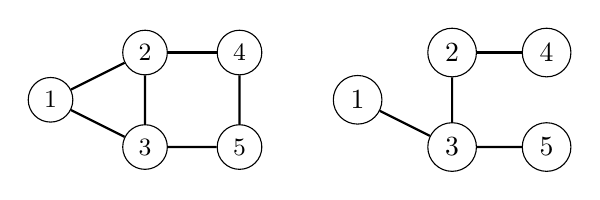
\begin{tikzpicture}[scale=0.6]
\begin{scope}
\small
\node[draw, circle] (1) at (0,-1) {$1$};
\node[draw, circle] (2) at (2,0) {$2$};
\node[draw, circle] (3) at (2,-2) {$3$};
\node[draw, circle] (4) at (4,0) {$4$};
\node[draw, circle] (5) at (4,-2) {$5$};
\path[draw,thick,-] (1) -- (2);
\path[draw,thick,-] (1) -- (3);
\path[draw,thick,-] (2) -- (3);
\path[draw,thick,-] (4) -- (5);
\path[draw,thick,-] (2) -- (4);
\path[draw,thick,-] (3) -- (5);
\end{scope}
\begin{scope}[xshift=6.5cm]
\node[draw, circle] (1) at (0,-1) {$1$};
\node[draw, circle] (2) at (2,0) {$2$};
\node[draw, circle] (3) at (2,-2) {$3$};
\node[draw, circle] (4) at (4,0) {$4$};
\node[draw, circle] (5) at (4,-2) {$5$};
%\path[draw,thick,-] (1) -- (2);
\path[draw,thick,-] (1) -- (3);
\path[draw,thick,-] (2) -- (3);
%\path[draw,thick,-] (4) -- (5);
\path[draw,thick,-] (2) -- (4);
\path[draw,thick,-] (3) -- (5);
\end{scope}
\end{tikzpicture}
\end{center}
\caption{Verkko ja yksi sen virittävistä puista.}
\label{fig:virpuu}
\end{figure}

Jos verkko on painotettu, kiinnostava ongelma on etsiä verkon
\emph{pienin virittävä puu}.
Tämä on virittävä puu, jonka kaarten painojen summa on
mahdollisimman pieni.
Esimerkiksi kuvassa \ref{fig:pievir} on painotettu verkko ja kaksi sen virittävää puuta,
joiden painot ovat 12 ja 10.
Näistä jälkimmäinen on verkon pienin virittävä puu.

\begin{figure}
\center
\begin{center}
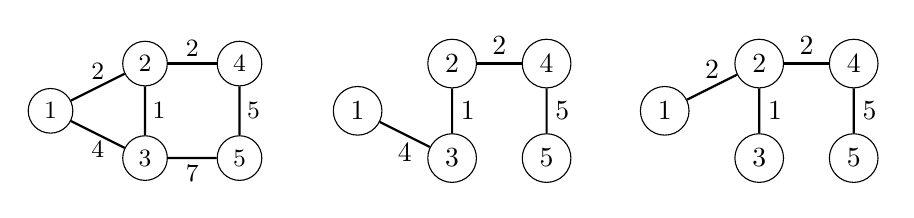
\begin{tikzpicture}[scale=0.6,label distance=-1.5mm]
\begin{scope}
\small
\node[draw, circle] (1) at (0,-1) {$1$};
\node[draw, circle] (2) at (2,0) {$2$};
\node[draw, circle] (3) at (2,-2) {$3$};
\node[draw, circle] (4) at (4,0) {$4$};
\node[draw, circle] (5) at (4,-2) {$5$};
\path[draw,thick,-] (1) -- node[font=\small,label=above:2] {} (2);
\path[draw,thick,-] (1) -- node[font=\small,label=below:4] {} (3);
\path[draw,thick,-] (2) -- node[font=\small,label=right:1] {} (3);
\path[draw,thick,-] (4) -- node[font=\small,label=right:5] {} (5);
\path[draw,thick,-] (2) -- node[font=\small,label=above:2] {} (4);
\path[draw,thick,-] (3) -- node[font=\small,label=below:7] {} (5);
\end{scope}
\begin{scope}[xshift=6.5cm]
\node[draw, circle] (1) at (0,-1) {$1$};
\node[draw, circle] (2) at (2,0) {$2$};
\node[draw, circle] (3) at (2,-2) {$3$};
\node[draw, circle] (4) at (4,0) {$4$};
\node[draw, circle] (5) at (4,-2) {$5$};
%\path[draw,thick,-] (1) -- node[font=\small,label=above:2] {} (2);
\path[draw,thick,-] (1) -- node[font=\small,label=below:4] {} (3);
\path[draw,thick,-] (2) -- node[font=\small,label=right:1] {} (3);
\path[draw,thick,-] (4) -- node[font=\small,label=right:5] {} (5);
\path[draw,thick,-] (2) -- node[font=\small,label=above:2] {} (4);
%\path[draw,thick,-] (3) -- node[font=\small,label=below:7] {} (5);
\end{scope}
\begin{scope}[xshift=13cm]
\node[draw, circle] (1) at (0,-1) {$1$};
\node[draw, circle] (2) at (2,0) {$2$};
\node[draw, circle] (3) at (2,-2) {$3$};
\node[draw, circle] (4) at (4,0) {$4$};
\node[draw, circle] (5) at (4,-2) {$5$};
\path[draw,thick,-] (1) -- node[font=\small,label=above:2] {} (2);
%\path[draw,thick,-] (1) -- node[font=\small,label=below:5] {} (3);
\path[draw,thick,-] (2) -- node[font=\small,label=right:1] {} (3);
\path[draw,thick,-] (4) -- node[font=\small,label=right:5] {} (5);
\path[draw,thick,-] (2) -- node[font=\small,label=above:2] {} (4);
%\path[draw,thick,-] (3) -- node[font=\small,label=below:7] {} (5);
\end{scope}
\end{tikzpicture}
\end{center}
\caption{Painotettu verkko ja kaksi virittävää puuta,
joiden painot ovat $4+1+2+5=12$ ja $2+1+2+5=10$.}
\label{fig:pievir}
\end{figure}

\subsection{Kruskalin algoritmi}

Kruskalin algoritmi muodostaa verkon
pienimmän virittävän puun aloittamalla tyhjästä verkosta,
jossa on vain verkon solmut, ja lisäämällä siihen kaaria.
Algoritmi käy läpi tarjolla olevat kaaret
järjestyksessä niiden painon mukaan kevyimmästä raskaimpaan.
Jokaisen kaaren kohdalla algoritmi ottaa kaaren mukaan,
jos se yhdistää kaksi eri komponenttia.
Kun kaikki komponentit on yhdistetty, pienin virittävä puu on valmis.

\begin{figure}
\center
\begin{center}
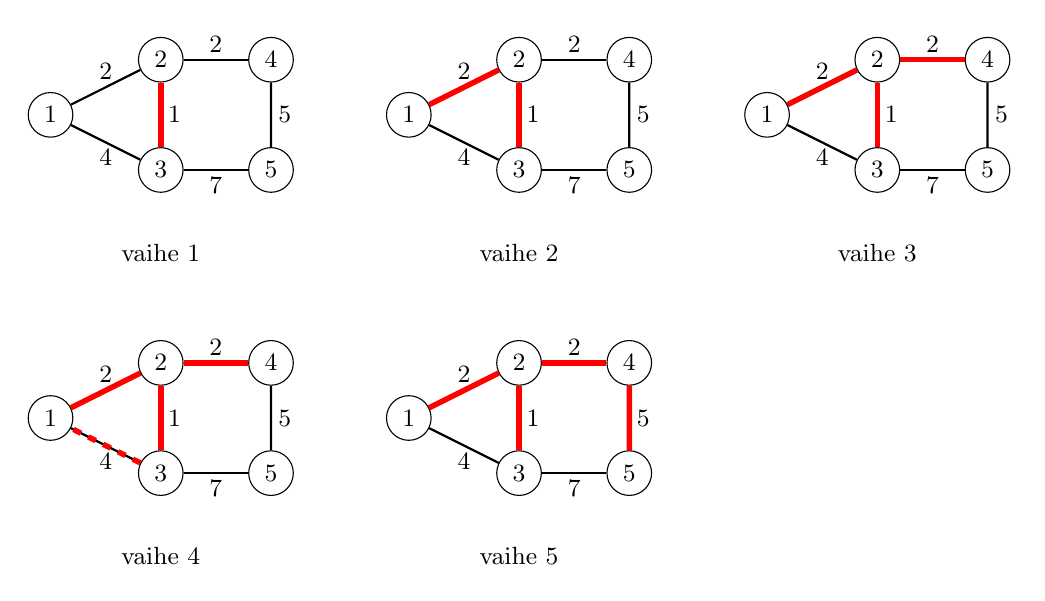
\begin{tikzpicture}[scale=0.7,label distance=-1.5mm]
\small
\newcommand\verkko[1]{
\node[draw, circle] (1) at (0,-1) {$1$};
\node[draw, circle] (2) at (2,0) {$2$};
\node[draw, circle] (3) at (2,-2) {$3$};
\node[draw, circle] (4) at (4,0) {$4$};
\node[draw, circle] (5) at (4,-2) {$5$};
\path[draw,thick,-] (1) -- node[font=\small,label=above:2] {} (2);
\path[draw,thick,-] (1) -- node[font=\small,label=below:4] {} (3);
\path[draw,thick,-] (2) -- node[font=\small,label=right:1] {} (3);
\path[draw,thick,-] (4) -- node[font=\small,label=right:5] {} (5);
\path[draw,thick,-] (2) -- node[font=\small,label=above:2] {} (4);
\path[draw,thick,-] (3) -- node[font=\small,label=below:7] {} (5);
\node at (2,-3.5) {vaihe #1};
}
\begin{scope}
\verkko{1}
\path[draw,thick,-,red,line width=2pt] (2) -- (3);
\end{scope}
\begin{scope}[xshift=6.5cm]
\verkko{2}
\path[draw,thick,-,red,line width=2pt] (2) -- (3);
\path[draw,thick,-,red,line width=2pt] (1) -- (2);
\end{scope}
\begin{scope}[xshift=13cm]
\verkko{3}
\path[draw,thick,-,red,line width=2pt] (2) -- (3);
\path[draw,thick,-,red,line width=2pt] (1) -- (2);
\path[draw,thick,-,red,line width=2pt] (2) -- (4);
\end{scope}
\begin{scope}[yshift=-5.5cm]
\verkko{4}
\path[draw,thick,-,red,line width=2pt] (2) -- (3);
\path[draw,thick,-,red,line width=2pt] (1) -- (2);
\path[draw,thick,-,red,line width=2pt] (2) -- (4);
\path[draw,thick,-,red,line width=2pt,dashed] (3) -- (1);
\end{scope}
\begin{scope}[yshift=-5.5cm,xshift=6.5cm]
\verkko{5}
\path[draw,thick,-,red,line width=2pt] (2) -- (3);
\path[draw,thick,-,red,line width=2pt] (1) -- (2);
\path[draw,thick,-,red,line width=2pt] (2) -- (4);
\path[draw,thick,-,red,line width=2pt] (4) -- (5);
\end{scope}
\end{tikzpicture}
\end{center}
\caption{Esimerkki Kruskalin algoritmin toiminnasta.}
\label{fig:kruesi}
\end{figure}

Kuva \ref{fig:kruesi} näyttää, kuinka Kruskalin algoritmi löytää pienimmän virittävän
puun esimerkkiverkossamme.
Verkon kaaret järjestyksessä kevyim\-mästä raskaimpaan ovat:

\begin{center}
\begin{tabular}{rr}
kaari & paino \\
\hline
$(2,3)$ & $1$ \\
$(1,2)$ & $2$ \\
$(2,4)$ & $2$ \\
$(1,3)$ & $4$ \\
$(4,5)$ & $5$ \\
$(3,5)$ & $7$ \\
\end{tabular}
\end{center}

Algoritmi käsittelee ensin kaaren $(2,3)$.
Solmut $2$ ja $3$ ovat eri komponenteissa,
joten kaari otetaan mukaan puuhun.
Tämän jälkeen algoritmi käsittelee kaaret $(1,2)$ ja $(2,4)$,
jotka valitaan myös puuhun.
Seuraavaksi vuorossa on kaari $(1,3)$,
mutta tämä kaari ei tule puuhun,
koska solmut $1$ ja $3$ ovat jo samassa komponentissa.
Lopuksi algoritmi ottaa mukaan kaaren $(4,5)$,
jolloin pienin virittävä puu on valmis.

Voimme toteuttaa Kruskalin algoritmin tehokkaasti
käyttäen union-find-rakennetta.
Algoritmin alussa järjestämme kaaret painojärjestykseen,
missä kuluu aikaa $O(m \log m)$.
Tämän jälkeen käymme kaaret läpi, ja jokaisen kaaren
kohdalla otamme kaaren mukaan, jos se yhdistää kaksi eri komponenttia.
Tässä kuluu aikaa $O(m \log n)$,
kun käytämme union-find-rakennetta.
Algoritmi vie siis yhteensä aikaa $O(m \log m)$.

\subsection{Primin algoritmi}

Primin algoritmi tarjoaa toisen lähestymistavan
pienimmän virittävän puun muodostamiseen.
Algoritmi aloittaa puun muodostamisen tilanteesta,
jossa puussa on vain yksi solmu.
Tämän jälkeen se etsii joka vaiheessa kevyimmän kaaren,
jonka toinen päätesolmu kuuluu puuhun ja toinen
päätesolmu on vielä puun ulkopuolella, ja lisää puuhun tämän kaaren.
Kun kaikki solmut on lisätty puuhun, pienin virittävä puu on valmis.

\begin{figure}
\center
\begin{center}
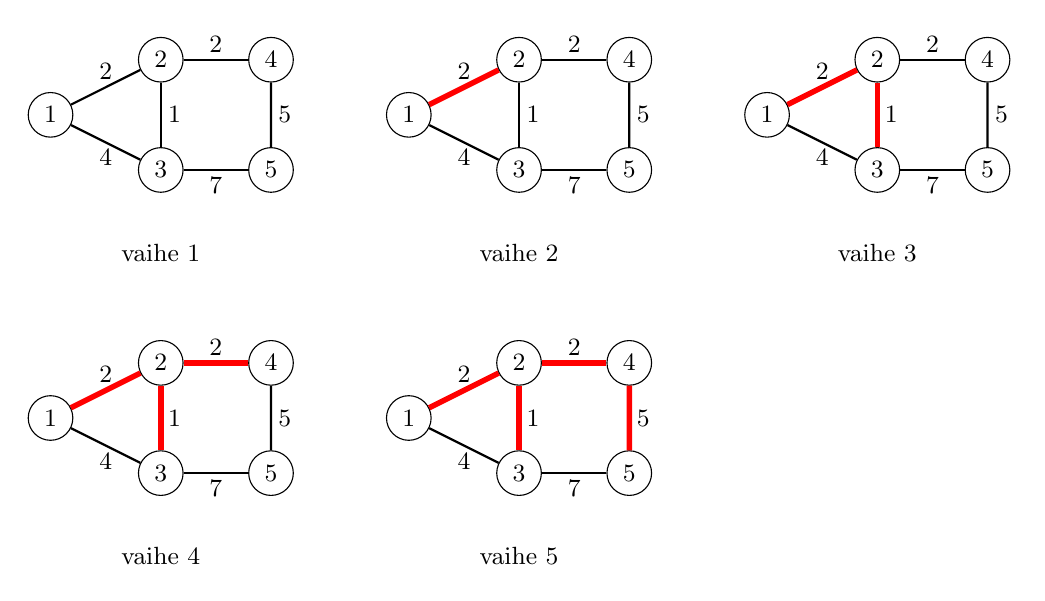
\begin{tikzpicture}[scale=0.7,label distance=-1.5mm]
\small
\newcommand\verkko[1]{
\node[draw, circle] (1) at (0,-1) {$1$};
\node[draw, circle] (2) at (2,0) {$2$};
\node[draw, circle] (3) at (2,-2) {$3$};
\node[draw, circle] (4) at (4,0) {$4$};
\node[draw, circle] (5) at (4,-2) {$5$};
\path[draw,thick,-] (1) -- node[font=\small,label=above:2] {} (2);
\path[draw,thick,-] (1) -- node[font=\small,label=below:4] {} (3);
\path[draw,thick,-] (2) -- node[font=\small,label=right:1] {} (3);
\path[draw,thick,-] (4) -- node[font=\small,label=right:5] {} (5);
\path[draw,thick,-] (2) -- node[font=\small,label=above:2] {} (4);
\path[draw,thick,-] (3) -- node[font=\small,label=below:7] {} (5);
\node at (2,-3.5) {vaihe #1};
}
\begin{scope}
\verkko{1}
\end{scope}
\begin{scope}[xshift=6.5cm]
\verkko{2}
\path[draw,thick,-,red,line width=2pt] (1) -- (2);
\end{scope}
\begin{scope}[xshift=13cm]
\verkko{3}
\path[draw,thick,-,red,line width=2pt] (1) -- (2);
\path[draw,thick,-,red,line width=2pt] (2) -- (3);
\end{scope}
\begin{scope}[yshift=-5.5cm]
\verkko{4}
\path[draw,thick,-,red,line width=2pt] (1) -- (2);
\path[draw,thick,-,red,line width=2pt] (2) -- (3);
\path[draw,thick,-,red,line width=2pt] (2) -- (4);
\end{scope}
\begin{scope}[yshift=-5.5cm,xshift=6.5cm]
\verkko{5}
\path[draw,thick,-,red,line width=2pt] (1) -- (2);
\path[draw,thick,-,red,line width=2pt] (2) -- (3);
\path[draw,thick,-,red,line width=2pt] (2) -- (4);
\path[draw,thick,-,red,line width=2pt] (4) -- (5);
\end{scope}
\end{tikzpicture}
\end{center}
\caption{Esimerkki Primin algoritmin toiminnasta.}
\label{fig:priesi}
\end{figure}

Kuva \ref{fig:priesi} näyttää esimerkin Primin algoritmin toiminnasta.
Voimme aloittaa puun rakentamisen mistä tahansa solmusta;
tässä esimerkissä aloitamme solmusta $1$.
Solmuun $1$ on yhteydessä kaksi kaarta $(1,2)$ ja $(1,3)$,
joista valitsemme kaaren $(1,2)$, koska se on kevyempi.
Seuraavaksi tarjolla ovat kaaret $(1,3)$, $(2,3)$ ja $(2,4)$,
joista valitsemme kaaren $(2,3)$.
Tämän jälkeen lisäämme puuhun vastaavalla tavalla kaaret
$(2,4)$, $(4,5)$, minkä jälkeen pienin virittävä puu on valmis.

Primin algoritmi muistuttaa paljon Dijkstran algoritmia.
Erona on, että Dijkstran algoritmissa valitsemme
seuraavaksi solmun, jonka etäisyys \emph{alkusolmuun} on pienin,
mutta Primin algoritmissa valitsemme solmun, jonka etäisyys
\emph{johonkin solmuun} puussa on pienin.
Voimme myös toteuttaa Primin algoritmin tehokkaasti samaan
tapaan kuin Dijkstran algoritmin keon avulla,
jolloin algoritmi vie aikaa $O(m \log n)$.

\subsection{Miksi algoritmit toimivat?}

Kruskalin ja Primin algoritmit ovat ahneita algoritmeja:
ne lisäävät joka askeleella kevyimmän mahdollisen kaaren puuhun.
Miksi on varmaa, että algoritmit tuottavat pienimmän virittävän
puun joka tilanteessa?

Voimme ajatella asiaa näin: 
Jos meillä on kaksi solmua $a$ ja $b$, jotka ovat eri komponenteissa,
meidän on yhdistettävä ne jotenkin samaan komponenttiin algoritmin aikana.
Jos kevyin saatavilla oleva kaari on solmujen $a$ ja $b$ välillä,
meidän kannattaa valita se, koska muuten joutuisimme yhdistämään komponentit
myöhemmin käyttäen raskaampaa kaarta.

Tarkastellaan esimerkkinä Kruskalin algoritmin alkua:
mitä tapahtuu, jos emme valitse puuhun kevyintä kaarta?
Kuvassa \ref{fig:pietod} näkyy kuvitteellinen tilanne,
jossa katkoviivoilla esitetty pienin virittävä puu ei sisällä
kevyintä kaarta $(2,3)$, jonka paino on 1.
Ei ole kuitenkaan mahdollista, että tämä olisi todellisuudessa
pienin virittävä puu, koska voisimme vaihtaa jonkin puun kaaren
kaareen $(2,3)$, jolloin puun paino pienenee.
Tämä tarkoittaa, että on varmasti turvallinen ratkaisu valita
kevyin kaari puuhun Kruskalin algoritmin alussa.
Vastaavasti voimme perustella, miksi tämän jälkeen kannattaa
valita seuraavaksi kevyin kaari, jne.

\begin{figure}
\center
\begin{center}
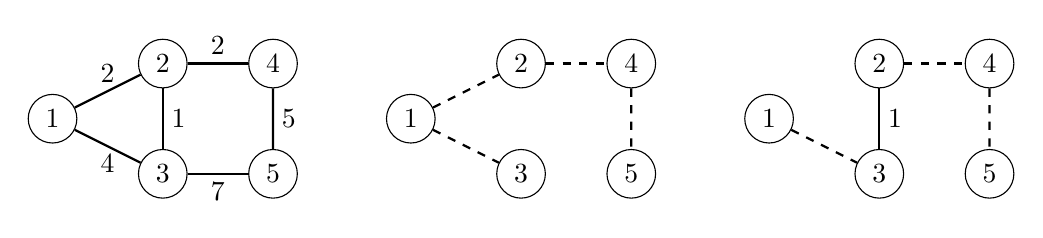
\begin{tikzpicture}[scale=0.7,label distance=-1.5mm]
\begin{scope}
\node[draw, circle] (1) at (0,-1) {$1$};
\node[draw, circle] (2) at (2,0) {$2$};
\node[draw, circle] (3) at (2,-2) {$3$};
\node[draw, circle] (4) at (4,0) {$4$};
\node[draw, circle] (5) at (4,-2) {$5$};
\path[draw,thick,-] (1) -- node[font=\small,label=above:2] {} (2);
\path[draw,thick,-] (1) -- node[font=\small,label=below:4] {} (3);
\path[draw,thick,-] (2) -- node[font=\small,label=right:1] {} (3);
\path[draw,thick,-] (4) -- node[font=\small,label=right:5] {} (5);
\path[draw,thick,-] (2) -- node[font=\small,label=above:2] {} (4);
\path[draw,thick,-] (3) -- node[font=\small,label=below:7] {} (5);
\end{scope}
\begin{scope}[xshift=6.5cm]
\node[draw, circle] (1) at (0,-1) {$1$};
\node[draw, circle] (2) at (2,0) {$2$};
\node[draw, circle] (3) at (2,-2) {$3$};
\node[draw, circle] (4) at (4,0) {$4$};
\node[draw, circle] (5) at (4,-2) {$5$};
\path[draw,thick,-,dashed] (1) -- (2);
\path[draw,thick,-,dashed] (1) -- (3);
\path[draw,thick,-,dashed] (4) -- (5);
\path[draw,thick,-,dashed] (2) -- (4);
\end{scope}
\begin{scope}[xshift=13cm]
\node[draw, circle] (1) at (0,-1) {$1$};
\node[draw, circle] (2) at (2,0) {$2$};
\node[draw, circle] (3) at (2,-2) {$3$};
\node[draw, circle] (4) at (4,0) {$4$};
\node[draw, circle] (5) at (4,-2) {$5$};
\path[draw,thick,-,dashed] (1) -- (3);
\path[draw,thick,-] (2) -- node[font=\small,label=right:1] {} (3);
\path[draw,thick,-,dashed] (4) -- (5);
\path[draw,thick,-,dashed] (2) -- (4);
\end{scope}
\end{tikzpicture}
\end{center}
\caption{Pienin virittävä puu sisältää varmasti kaaren $(2,3)$,
koska muuten voisimme pienentää puun painoa valitsemalla sen.}
\label{fig:pietod}
\end{figure}

\chapter{Virtauslaskenta}

Lähtökohtanamme on suunnattu verkko, jossa on kaksi erityistä solmua:
\emph{lähtösolmu} ja \emph{kohdesolmu}.
Jokaisella kaarella on paino, joka rajoittaa,
miten paljon virtausta voi kulkea kaarta pitkin,
ja haluamme selvittää, mikä on \emph{maksimivirtaus} lähtösolmusta
kohdesolmuun.

Lähtökohtanamme on suunnattu verkko, jossa on kaksi erityistä solmua:
\emph{lähtösolmu} ja \emph{kohdesolmu}.
Jokaisella kaarella on paino, joka rajoittaa,
miten paljon virtausta voi kulkea kaarta pitkin,
ja haluamme selvittää, mikä on \emph{maksimivirtaus} lähtösolmusta
kohdesolmuun.

\section{Maksimivirtaus}

Maksimivirtausongelmassa haluamme selvittää
suurimman \emph{virtauksen} suunnatun verkon
lähtösolmusta kohdesolmuun.
Virtaus lähtee liikkeelle lähtö\-solmusta ja saapuu kohdesolmuun
niin, että jokaiseen välisolmuun tuleva virtaus on
yhtä suuri kuin solmusta lähtevä virtaus.
Jokaisella kaarella on \emph{kapasiteetti}, jota virtauksen
määrä kaarta pitkin ei saa ylittää.

\begin{figure}
\center
\begin{center}
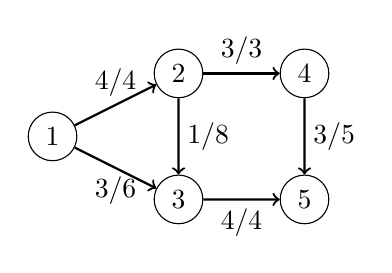
\begin{tikzpicture}[scale=0.8,label distance=-1.5mm]
\node[draw, circle] (1) at (0,-1) {$1$};
\node[draw, circle] (2) at (2,0) {$2$};
\node[draw, circle] (3) at (2,-2) {$3$};
\node[draw, circle] (4) at (4,0) {$4$};
\node[draw, circle] (5) at (4,-2) {$5$};
\path[draw,thick,->] (1) -- node[font=\small,label=above:$4/4$] {} (2);
\path[draw,thick,->] (1) -- node[font=\small,label=below:$3/6$] {} (3);
\path[draw,thick,->] (2) -- node[font=\small,label=right:$1/8$] {} (3);
\path[draw,thick,->] (2) -- node[font=\small,label=above:$3/3$] {} (4);
\path[draw,thick,->] (3) -- node[font=\small,label=below:$4/4$] {} (5);
\path[draw,thick,->] (4) -- node[font=\small,label=right:$3/5$] {} (5);
\end{tikzpicture}
\end{center}
\caption{Maksimivirtaus solmusta $1$ solmuun $5$ on $7$.}
\label{fig:makvir}
\end{figure}

Tarkastellaan esimerkkinä kuvan \ref{fig:makvir} verkkoa.
Tässä verkossa maksimivirtaus solmusta $1$ solmuun $5$ on $7$.
Jokaisessa kaaressa merkintä $v/k$ tarkoittaa,
että kaaren kautta kulkee virtausta $v$ ja
kaaren kapasiteetti on $k$.
Solmusta $1$ lähtevä virtauksen määrä on $4+3=7$,
solmuun $5$ saapuva virtauksen määrä on $3+4=7$
ja kaikissa muissa solmuissa saapuva virtaus
on yhtä suuri kuin lähtevä virtaus.

\subsection{Ford-Fulkersonin algoritmi}

Ford-Fulkersonin algoritmi on tunnetuin menetelmä verkon
maksimivirtauksen etsimiseen,
ja tutustumme seuraavaksi tämän algoritmin toimintaan.
Algoritmi etsii polkuja lähtösolmusta kohdesolmuun,
jotka kasvattavat virtausta pikkuhiljaa.
Kun mitään polkua ei voi enää muodostaa, algoritmi on onnistunut
muodostamaan maksimivirtauksen.

\begin{figure}
\center
\begin{center}
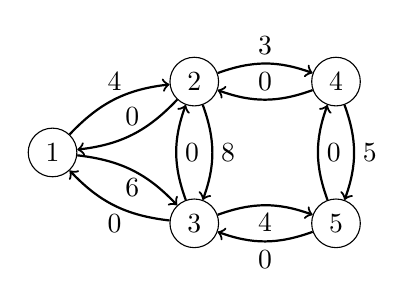
\begin{tikzpicture}[scale=0.9,label distance=-1.5mm]
\node[draw, circle] (1) at (0,-1) {$1$};
\node[draw, circle] (2) at (2,0) {$2$};
\node[draw, circle] (3) at (2,-2) {$3$};
\node[draw, circle] (4) at (4,0) {$4$};
\node[draw, circle] (5) at (4,-2) {$5$};
\path[draw,thick,->] (1) edge [bend left=20] node[font=\small,label=above:$4$] {} (2);
\path[draw,thick,->] (2) edge [bend left=20] node[font=\small,label=above:$0$] {} (1);
\path[draw,thick,->] (1) edge [bend left=20] node[font=\small,label=below:$6$] {} (3);
\path[draw,thick,->] (3) edge [bend left=20] node[font=\small,label=below:$0$] {} (1);
\path[draw,thick,->] (2) edge [bend left=20] node[font=\small,label=right:$8$] {} (3);
\path[draw,thick,->] (3) edge [bend left=20] node[font=\small,label=right:$0$] {} (2);
\path[draw,thick,->] (2) edge [bend left=20] node[font=\small,label=above:$3$] {} (4);
\path[draw,thick,->] (4) edge [bend left=20] node[font=\small,label=above:$0$] {} (2);
\path[draw,thick,->] (3) edge [bend left=20] node[font=\small,label=below:$4$] {} (5);
\path[draw,thick,->] (5) edge [bend left=20] node[font=\small,label=below:$0$] {} (3);
\path[draw,thick,->] (4) edge [bend left=20] node[font=\small,label=right:$5$] {} (5);
\path[draw,thick,->] (5) edge [bend left=20] node[font=\small,label=right:$0$] {} (4);
\end{tikzpicture}
\end{center}
\caption{Verkon esitysmuoto Ford-Fulkersonin algoritmissa.}
\label{fig:floesi}
\end{figure}

Algoritmin käyttäminen vaatii, että verkko on esitetty
erityisessä muodossa, jossa jokaista alkuperäisen verkon
kaarta vastaa kaksi kaarta:
alkuperäinen kaari, jonka painona on aluksi kaaren kapasiteetti,
sekä sille kään\-teinen kaari, jonka painona on aluksi $0$.
Käänteisten kaarten avulla pystymme tarvittaessa \emph{peruuttamaan}
virtausta algoritmin aikana.
Kuva \ref{fig:floesi} näyttää, kuinka esitämme esimerkkiverkkomme algoritmissa.

Algoritmin jokaisessa vaiheessa muodostamme polun
lähtösolmusta kohdesolmuun.
Polku voi olla mikä tahansa, kunhan jokaisen kaaren paino
polulla on positiivinen.
Polun muodostamisen jälkeen virtaus lähtösolmusta kohdesolmuun
kasvaa $p$:llä, missä $p$ on pienin kaaren paino polulla.
Lisäksi jokaisen polulla olevan kaaren paino vähenee $p$:llä
ja jokaisen niille käänteisen kaaren paino kasvaa $p$:llä.
Etsimme vastaavasti uusia polkuja, kunnes mitään sallittua
polkua ei voi enää muodostaa.

Kuva \ref{fig:floesi} näyttää, kuinka Ford-Fulkersonin algoritmi muodostaa
maksimivirtauksen esimerkkiverkossamme.
Algoritmi muodostaa ensin polun $1 \rightarrow 2 \rightarrow 3 \rightarrow 5$,
jossa pienin paino on $4$.
Tämän seurauksena virtaus kasvaa $4$:llä,
polulla olevien kaarten paino vähenee $4$:llä
ja käänteisten kaarten paino kasvaa $4$:llä.
Tämän jälkeen algoritmi muodostaa polun
$1 \rightarrow 3 \rightarrow 2 \rightarrow 4 \rightarrow 5$,
joka kasvattaa virtausta $3$:lla.
Huomaa, että tämä polku peruuttaa
kaarta $2 \rightarrow 3$ menevää virtausta,
koska se kulkee käänteisen kaaren $3 \rightarrow 2$ kautta.
Tämän jälkeen algoritmi ei enää pysty muodostamaan mitään polkua
solmusta $1$ solmuun $5$, joten maksimivirtaus on $4+3=7$.

\begin{figure}
\center
\begin{center}
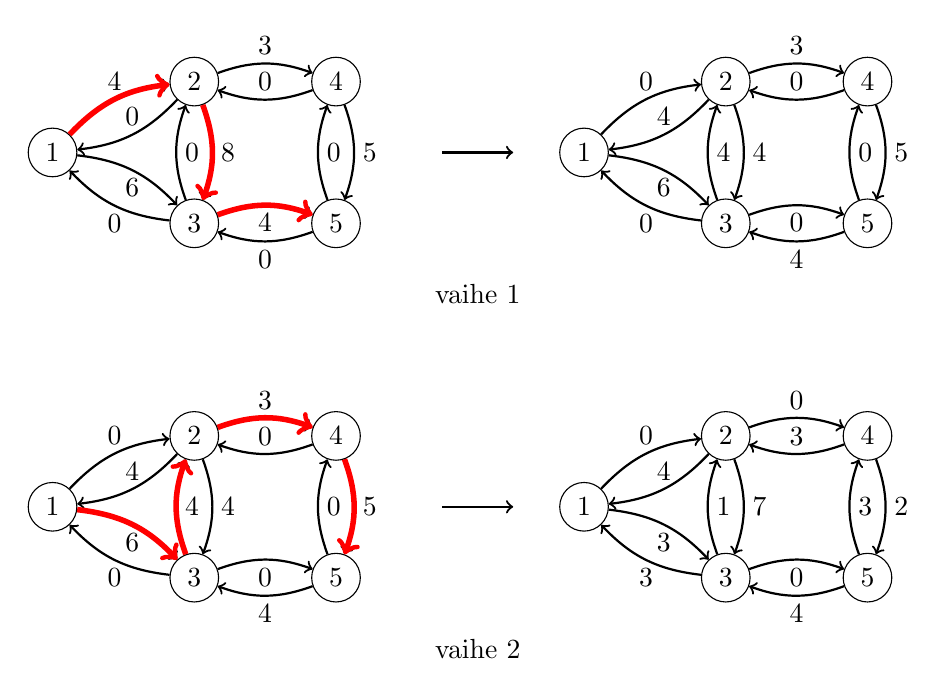
\begin{tikzpicture}[scale=0.9,label distance=-1.5mm]
\newcommand\verkko[0]{
\node[draw, circle] (1) at (0,-1) {$1$};
\node[draw, circle] (2) at (2,0) {$2$};
\node[draw, circle] (3) at (2,-2) {$3$};
\node[draw, circle] (4) at (4,0) {$4$};
\node[draw, circle] (5) at (4,-2) {$5$};
}
\begin{scope}
\verkko
\path[draw,thick,->] (1) edge [bend left=20] node[font=\small,label=above:$4$] {} (2);
\path[draw,thick,->] (2) edge [bend left=20] node[font=\small,label=above:$0$] {} (1);
\path[draw,thick,->] (1) edge [bend left=20] node[font=\small,label=below:$6$] {} (3);
\path[draw,thick,->] (3) edge [bend left=20] node[font=\small,label=below:$0$] {} (1);
\path[draw,thick,->] (2) edge [bend left=20] node[font=\small,label=right:$8$] {} (3);
\path[draw,thick,->] (3) edge [bend left=20] node[font=\small,label=right:$0$] {} (2);
\path[draw,thick,->] (2) edge [bend left=20] node[font=\small,label=above:$3$] {} (4);
\path[draw,thick,->] (4) edge [bend left=20] node[font=\small,label=above:$0$] {} (2);
\path[draw,thick,->] (3) edge [bend left=20] node[font=\small,label=below:$4$] {} (5);
\path[draw,thick,->] (5) edge [bend left=20] node[font=\small,label=below:$0$] {} (3);
\path[draw,thick,->] (4) edge [bend left=20] node[font=\small,label=right:$5$] {} (5);
\path[draw,thick,->] (5) edge [bend left=20] node[font=\small,label=right:$0$] {} (4);
\path[draw,thick,->,red,line width=2pt] (1) edge [bend left=20] (2);
\path[draw,thick,->,red,line width=2pt] (2) edge [bend left=20] (3);
\path[draw,thick,->,red,line width=2pt] (3) edge [bend left=20] (5);
\draw[->,thick] (5.5,-1) -- (6.5,-1);
\node at (6,-3) {vaihe 1};
\end{scope}
\begin{scope}[xshift=7.5cm]
\verkko
\path[draw,thick,->] (1) edge [bend left=20] node[font=\small,label=above:$0$] {} (2);
\path[draw,thick,->] (2) edge [bend left=20] node[font=\small,label=above:$4$] {} (1);
\path[draw,thick,->] (1) edge [bend left=20] node[font=\small,label=below:$6$] {} (3);
\path[draw,thick,->] (3) edge [bend left=20] node[font=\small,label=below:$0$] {} (1);
\path[draw,thick,->] (2) edge [bend left=20] node[font=\small,label=right:$4$] {} (3);
\path[draw,thick,->] (3) edge [bend left=20] node[font=\small,label=right:$4$] {} (2);
\path[draw,thick,->] (2) edge [bend left=20] node[font=\small,label=above:$3$] {} (4);
\path[draw,thick,->] (4) edge [bend left=20] node[font=\small,label=above:$0$] {} (2);
\path[draw,thick,->] (3) edge [bend left=20] node[font=\small,label=below:$0$] {} (5);
\path[draw,thick,->] (5) edge [bend left=20] node[font=\small,label=below:$4$] {} (3);
\path[draw,thick,->] (4) edge [bend left=20] node[font=\small,label=right:$5$] {} (5);
\path[draw,thick,->] (5) edge [bend left=20] node[font=\small,label=right:$0$] {} (4);
\end{scope}
\begin{scope}[yshift=-5cm]
\verkko
\path[draw,thick,->] (1) edge [bend left=20] node[font=\small,label=above:$0$] {} (2);
\path[draw,thick,->] (2) edge [bend left=20] node[font=\small,label=above:$4$] {} (1);
\path[draw,thick,->] (1) edge [bend left=20] node[font=\small,label=below:$6$] {} (3);
\path[draw,thick,->] (3) edge [bend left=20] node[font=\small,label=below:$0$] {} (1);
\path[draw,thick,->] (2) edge [bend left=20] node[font=\small,label=right:$4$] {} (3);
\path[draw,thick,->] (3) edge [bend left=20] node[font=\small,label=right:$4$] {} (2);
\path[draw,thick,->] (2) edge [bend left=20] node[font=\small,label=above:$3$] {} (4);
\path[draw,thick,->] (4) edge [bend left=20] node[font=\small,label=above:$0$] {} (2);
\path[draw,thick,->] (3) edge [bend left=20] node[font=\small,label=below:$0$] {} (5);
\path[draw,thick,->] (5) edge [bend left=20] node[font=\small,label=below:$4$] {} (3);
\path[draw,thick,->] (4) edge [bend left=20] node[font=\small,label=right:$5$] {} (5);
\path[draw,thick,->] (5) edge [bend left=20] node[font=\small,label=right:$0$] {} (4);
\path[draw,thick,->,red,line width=2pt] (1) edge [bend left=20] (3);
\path[draw,thick,->,red,line width=2pt] (3) edge [bend left=20] (2);
\path[draw,thick,->,red,line width=2pt] (2) edge [bend left=20] (4);
\path[draw,thick,->,red,line width=2pt] (4) edge [bend left=20] (5);
\draw[->,thick] (5.5,-1) -- (6.5,-1);
\node at (6,-3) {vaihe 2};
\end{scope}
\begin{scope}[yshift=-5cm,xshift=7.5cm]
\verkko
\path[draw,thick,->] (1) edge [bend left=20] node[font=\small,label=above:$0$] {} (2);
\path[draw,thick,->] (2) edge [bend left=20] node[font=\small,label=above:$4$] {} (1);
\path[draw,thick,->] (1) edge [bend left=20] node[font=\small,label=below:$3$] {} (3);
\path[draw,thick,->] (3) edge [bend left=20] node[font=\small,label=below:$3$] {} (1);
\path[draw,thick,->] (2) edge [bend left=20] node[font=\small,label=right:$7$] {} (3);
\path[draw,thick,->] (3) edge [bend left=20] node[font=\small,label=right:$1$] {} (2);
\path[draw,thick,->] (2) edge [bend left=20] node[font=\small,label=above:$0$] {} (4);
\path[draw,thick,->] (4) edge [bend left=20] node[font=\small,label=above:$3$] {} (2);
\path[draw,thick,->] (3) edge [bend left=20] node[font=\small,label=below:$0$] {} (5);
\path[draw,thick,->] (5) edge [bend left=20] node[font=\small,label=below:$4$] {} (3);
\path[draw,thick,->] (4) edge [bend left=20] node[font=\small,label=right:$2$] {} (5);
\path[draw,thick,->] (5) edge [bend left=20] node[font=\small,label=right:$3$] {} (4);
\end{scope}
\end{tikzpicture}
\end{center}
\caption{Esimerkki Ford-Fulkersonin algoritmin toiminnasta.}
\label{fig:floesi}
\end{figure}

\subsection{Yhteys minimileikkaukseen}

Ford-Fulkersonin algoritmin toimintaidea on sinänsä järkevä,
mutta ei ole silti päältä päin todellakaan selvää,
miksi algoritmi löytää varmasti maksimivirtauksen.
Jotta voimme ymmärtää paremmin algoritmin toimintaa,
tarkastelemme seuraavaksi toista verkko-ongelmaa,
joka antaa meille uuden näkökulman maksimivirtaukseen.

Lähtökohtanamme on edelleen suunnattu verkko,
jossa on lähtösolmu ja kohdesolmu.
Sanomme, että joukko kaaria muodostaa \emph{leikkauksen},
jos niiden poistaminen verkosta estää kulkemisen
lähtösolmusta kohdesolmuun.
\emph{Minimileikkaus} on puolestaan leikkaus,
jossa kaarten yhteispaino on mahdollisimman pieni.
Kuvassa \ref{fig:minlei} näkyy esimerkkiverkkomme minimileikkaus,
jossa poistamme kaaret $2 \rightarrow 4$ ja $3 \rightarrow 5$
ja jonka paino on $3+4=7$.

\begin{figure}
\center
\begin{center}
\begin{tikzpicture}[scale=0.8,label distance=-1.5mm]
\node[draw, circle] (1) at (0,-1) {$1$};
\node[draw, circle] (2) at (2,0) {$2$};
\node[draw, circle] (3) at (2,-2) {$3$};
\node[draw, circle] (4) at (4,0) {$4$};
\node[draw, circle] (5) at (4,-2) {$5$};
\path[draw,thick,->] (1) -- node[font=\small,label=above:$4$] {} (2);
\path[draw,thick,->] (1) -- node[font=\small,label=below:$6$] {} (3);
\path[draw,thick,->] (2) -- node[font=\small,label=right:$8$] {} (3);
\path[draw,thick,->] (2) -- node[font=\small,label=above:$3$] {} (4);
\path[draw,thick,->] (3) -- node[font=\small,label=below:$4$] {} (5);
\path[draw,thick,->] (4) -- node[font=\small,label=right:$5$] {} (5);
\path[draw,thick,-,red,line width=2pt] (2.75,-0.25) -- (3.25,0.25);
\path[draw,thick,-,red,line width=2pt] (2.75,0.25) -- (3.25,-0.25);
\path[draw,thick,-,red,line width=2pt] (2.75,-2.25) -- (3.25,-1.75);
\path[draw,thick,-,red,line width=2pt] (2.75,-1.75) -- (3.25,-2.25);
\end{tikzpicture}
\end{center}
\caption{Minimileikkaus, jossa poistamme kaaret $2 \rightarrow 4$ ja $3 \rightarrow 5$.}
\label{fig:minlei}
\end{figure}

Osoittautuu, että verkon maksimivirtaus on aina yhtä suuri kuin
minimileikkaus, ja tämä yhteys auttaa perustelemaan,
miksi Ford-Fulkersonin algoritmi toimii.
Ensinnäkin voimme havaita, että \emph{mikä tahansa}
verkon leikkaus on yhtä suuri tai suurempi
kuin maksimivirtaus.
Tämä johtuu siitä, että virtauksen täytyy ylittää
leikkaukseen kuuluvat kaaret, jotta se pääsee
lähtösolmusta kohdesolmuun.
Esimerkiksi kuvassa \ref{fig:minlei} virtaus voi
päästä solmusta $1$ solmuun $5$
joko kulkemalla kaarta $2 \rightarrow 4$ tai kaarta $3 \rightarrow 5$.
Niinpä virtaus ei voi olla suurempi kuin näiden kaarten
painojen summa.

\begin{figure}
\center
\begin{center}
\begin{tikzpicture}[scale=0.9,label distance=-1.5mm]
\node[draw, circle, fill=lightgray] (1) at (0,-1) {$1$};
\node[draw, circle, fill=lightgray] (2) at (2,0) {$2$};
\node[draw, circle, fill=lightgray] (3) at (2,-2) {$3$};
\node[draw, circle] (4) at (4,0) {$4$};
\node[draw, circle] (5) at (4,-2) {$5$};
\path[draw,thick,->] (1) edge [bend left=20] node[font=\small,label=above:$0$] {} (2);
\path[draw,thick,->] (2) edge [bend left=20] node[font=\small,label=above:$4$] {} (1);
\path[draw,thick,->] (1) edge [bend left=20] node[font=\small,label=below:$3$] {} (3);
\path[draw,thick,->] (3) edge [bend left=20] node[font=\small,label=below:$3$] {} (1);
\path[draw,thick,->] (2) edge [bend left=20] node[font=\small,label=right:$7$] {} (3);
\path[draw,thick,->] (3) edge [bend left=20] node[font=\small,label=right:$1$] {} (2);
\path[draw,thick,->] (2) edge [bend left=20] node[font=\small,label=above:$0$] {} (4);
\path[draw,thick,->] (4) edge [bend left=20] node[font=\small,label=above:$3$] {} (2);
\path[draw,thick,->] (3) edge [bend left=20] node[font=\small,label=below:$0$] {} (5);
\path[draw,thick,->] (5) edge [bend left=20] node[font=\small,label=below:$4$] {} (3);
\path[draw,thick,->] (4) edge [bend left=20] node[font=\small,label=right:$2$] {} (5);
\path[draw,thick,->] (5) edge [bend left=20] node[font=\small,label=right:$3$] {} (4);
\end{tikzpicture}
\end{center}
\caption{Solmut 1, 2 ja 3 ovat saavutettavissa lähtösolmusta.}
\label{fig:flolei}
\end{figure}

Toisaalta Ford-Fulkersonin algoritmi muodostaa sivutuotteenaan
myös verkon leikkauksen, joka on yhtä suuri kuin maksimivirtaus.
Löydämme leikkauksen etsimällä ensin kaikki solmut,
joihin pääsemme lähtösolmusta positiivisia kaaria pitkin
algoritmin lopputilanteessa.
Kuva \ref{fig:flolei} näyttää nämä solmut esimerkkiverkossamme:
solmut ovat 1, 2 ja 3.
Kun valitsemme sitten alkuperäisen verkon kaaret,
jotka johtavat näiden solmujen ulkopuolelle
ja joiden kapasiteetti on käytetty kokonaan,
saamme aikaan verkon leikkauksen.
Esimerkissämme nämä kaaret ovat $2 \rightarrow 4$ ja $3 \rightarrow 5$.

Koska olemme löytäneet virtauksen, joka on yhtä suuri kuin leikkaus,
ja toisaalta virtaus ei voi olla mitään leikkausta suurempi,
olemme siis löytäneet maksimivirtauksen ja minimileikkauksen,
joten Ford-Fulkersonin algoritmi toimii oikein.

\subsection{Polkujen valitseminen}

Voimme muodostaa Ford-Fulkersonin algoritmin aikana miten tahansa,
mutta polkujen valintatapa vaikuttaa algoritmin tehokkuuteen.
Pahimmassa tapauksessa jokainen polku tuottaa vain yhden yksikön
lisää virtausta, jolloin algoritmi joutuu muodostamaan kaikkiaan $f$ polkua,
missä $f$ on verkon maksimivirtaus.
Jos muodostamme polut syvyyshaulla, saamme siis algoritmin
ajankäytölle ylärajan $O(f (n+m))$.

Edmonds-Karpin algoritmi on Ford-Fulkersonin algoritmin versio,
jossa muodostammekin polut \emph{leveyshaulla}.
Tämä tarkoittaa, että valitsemme aina
polun, jossa on mahdollisimman vähän kaaria.
On mahdollista osoittaa, että tällaisen valinnan ansiosta
algoritmi muodostaa aina enintään $nm$ polkua ja
sen aikavaativuus on $O(nm (n+m))$.

\section{Sovelluksia}

Virtauslaskennan merkitys on siinä, että voimme \emph{palauttaa}
monia ongelmia maksimivirtauksen laskemiseen.
Tämä tarkoittaa, että muunnamme ongelman jotenkin
sellaiseen muotoon, että se vastaa maksimivirtauksen etsimistä.
Tutustumme seuraavaksi joihinkin tällaisiin ongelmiin.

\subsection{Erilliset polut}

\subsection{Maksimiparitus}

\subsection{X}

\chapter{NP-ongelmat}

Olemme tässä kirjassa tutustuneet menetelmiin, joiden avulla voimme
ratkaista tehokkaasti ongelmia.
Kuitenkin on myös monia ongelmia, joiden ratkaisemiseen ei tällä
hetkellä tunneta mitään tehokasta algoritmia.
Jos vastaamme tulee tällainen ongelma, hyvät neuvot ovat kalliit.

Vaikeiden ongelmien yhteydessä vastaan tulee usein
kirjainyhdistelmä NP.
Erityisen tunnettu on P vs. NP -ongelma,
jonka ratkaisijalle on luvattu miljoonan dollarin potti.
Hankalalta tuntuvasta ongelmasta saatetaan mainita, että
se on NP-täydellinen tai NP-vaikea.
Nyt on aika selvittää, mitä nämä käsitteet oikeastaan tarkoittavat.

\section{Luokat P ja NP}

Keskitymme tässä luvussa \emph{päätösongelmiin}, joissa algoritmin tulee
antaa vastaus ''kyllä'' tai ''ei''.
Esimerkiksi ongelma 
''onko verkossa polkua solmusta $a$ solmuun $b$?'' on päätösongelma.
Tulemme huomaamaan, että voimme muotoilla monenlaisia ongelmia
päätösongelmina eikä tämä rajoita juurikaan, mitä ongelmia voimme tarkastella.

\subsubsection{Luokka P}

Luokka P sisältää päätösongelmat, joiden ratkaisemiseen on
olemassa \emph{polynominen} algoritmi eli algoritmi, jonka aikavaativuus
on enintään $O(n^k)$, missä $k$ on vakio.
Lähes kaikki tässä kirjassa esitetyt algoritmit
ovat toimineet polyonmisessa ajassa.
Tuttuja polynomisia aikavaativuuksia ovat esimerkiksi
$O(1)$, $O(\log n)$ $O(n)$, $O(n \log n)$, $O(n^2)$ ja $O(n^3)$.

Esimerkiksi ongelma ''onko verkossa polkua solmusta $a$ solmuun $b$?''
kuuluu luokkaan P, koska voimme ratkaista sen monellakin tavalla
polynomisessa ajassa.
Voimme vaikkapa aloittaa syvyyshaun solmusta $a$ ja tarkastaa,
pääsemmekö solmuun $b$.
Tuloksena on algoritmi, jolla on polynominen aikavaativuus
$O(n+m)$, joten ongelma kuuluu luokkaan P.

Luokan P tarkoituksena on kuvata ongelmia, jotka voimme
ratkaista jossain mielessä \emph{tehokkaasti}.
Tässä tehokkuuden määritelmä on varsin karkea:
pidämme algoritmia tehokkaana, jos sillä on mikä tahansa
polynominen aikavaativuus.
Onko $O(n^{100})$-aikainen algoritmi siis tehokas?
Ei, mutta käytännössä vakio $k$ on yleensä pieni ja
on osoittautunut, että polynominen aikavaativuus 
on toimiva tehokkuuden mittari.


\subsubsection{Luokka NP}

Luokka NP sisältää päätösongelmat, joissa jokaisessa
''kyllä''-tapauksessa on olemassa
\emph{todiste}, jonka avulla voimme
\emph{tarkastaa} polynomisessa ajassa, että vastaus on oikein.
Todiste on merkkijono, jonka koko on polynominen
suhteessa syötteeseen,
ja se antaa meille lisätietoa siitä,
minkä takia ''kyllä''-vastaus pitää paikkansa syötteelle.

Esimerkki luokkaan NP kuuluvasta ongelmasta on
''onko verkossa polkua solmusta $a$ solmuun $b$,
joka kulkee tasan kerran jokaisen verkon solmun kautta?''.
Tämän ongelman ratkaisemiseen ei tunneta tehokasta algoritmia,
mutta jokaisessa ''kyllä''-tapauksessa on olemassa todiste:
halutunlainen polku solmusta $a$ solmuun $b$.
Voimme tarkastaa helposti polynomisessa ajassa,
että todisteen kuvaamalla polulla on vaaditut ominaisuudet.

Jos vastaus syötteeseen on ''ei'', tähän ei tarvitse
liittyä tehokkaasti tarkastettavaa todistetta.
Usein olisikin hankalaa antaa todiste siitä, että jotain
asiaa \emph{ei} ole olemassa.
Äskeisessä esimerkissä meidän oli helppoa todistaa
polun olemassaolo, koska voimme vain näyttää kyseisen polun,
mutta meillä ei ole vastaavaa keinoa todistaa, että polkua ei ole olemassa.

Huomaa, että kaikki luokan P ongelmat kuuluvat myös
luokkaan NP. Tämä johtuu siitä, että luokan P ongelmissa
voimme tarkastaa ''kyllä''-vastauksen
\emph{tyhjän} todisteen avulla: voimme saman tien ratkaista
koko ongelman alusta alkaen polynomisessa ajassa.

\subsubsection{P vs. NP}

Äkkiseltään tuntuu selvältä, että luokassa NP täytyy olla
enemmän ongelmia kuin luokassa P.
Luokassa NP meidän riittää vain pystyä tarkastamaan ''kyllä''-vastauksen
todiste, mikä tuntuu helpommalta kuin muodostaa ongelman ratkaisu tyhjästä.
Monet uskovatkin, että luokka NP on suurempi kuin luokka P --
mutta kukaan ei ole onnistunut todistamaan asiaa.

Tietojenkäsittelytieteen merkittävä avoin ongelma onkin,
päteekö $P=NP$ vai $P \neq NP$.
Monet tutkijat ovat tarttuneet haasteeseen
70-luvulta lähtien, mutta kaikki ovat epäonnistuneet.
Ongelman ratkaisija saisi maineen ja kunnian lisäksi
myös tuntuvan rahallisen korvauksen, koska
Clay-instituutti on luvannut miljoonan dollarin palkinnon
sille, joka todistaa, että $P=NP$ tai $P \neq NP$.
Voi olla kuitenkin, että tämä on yksi \emph{vaikeimmista}
tavoista ansaita miljoona dollaria.

Jos pätee $P \neq NP$, kuten uskotaan,
vaikeutena on keksiä keino todistaa, että jotakin
luokan NP ongelmaa on mahdotonta ratkaista
polynomisessa ajassa.
Tämän todistaminen on vaikeaa, koska meidän pitää näyttää,
että tehokasta algoritmia ei ole olemassa,
vaikka laatisimme algoritmin miten tahansa.
Vaikka moni on koettanut tuloksetta ratkoa
tunnettuja NP-ongelmia, kysymys saattaa silti olla siitä,
että tehokas algoritmi olisi olemassa mutta kukaan ei
vain ole vielä löytänyt sitä.

\section{NP-täydellisyys}

Sanomme, että ongelma on \emph{NP-täydellinen},
jos se kuuluu luokkaan NP ja mikä tahansa luokan NP
ongelma voidaan \emph{palauttaa} siihen polynomisessa ajassa.
NP-täydelliset ongelmat ovat luokan NP vaikeimpia ongelmia:
jos voisimme ratkaista jonkin NP-täydellisen ongelman tehokkaasti,
voisimme ratkaista minkä tahansa luokan NP ongelman tehokkaasti.

Kiinnostava ilmiö on, että lähes kaikki tunnetut luokan NP
ongelmat joko kuuluvat myös luokkaan P tai ovat
NP-täydellisiä.
Nykyään tunnetaankin tuhansia erilaisia NP-täydellisiä ongelmia.
Jos keksisimme mihin tahansa niistä polynomisessa ajassa toimivan
ratkaisun, olisimme samalla onnistuneet todistamaan, että $P=NP$.

\subsection{SAT-ongelma}

Ensimmäinen löydetty NP-täydellinen ongelma oli
SAT-ongelma, jossa annettuna on konjunktiivisessa
normaalimuodossa oleva looginen kaava ja haluamme
selvittää, voimmeko valita muuttujien arvot niin,
että kaava on tosi.
Konjunktiivinen normaalimuoto tarkoittaa,
että kaava koostuu lausekkeista, jotka on yhdistetty
ja-operaatiolla ($\land$), ja jokainen lauseke koostuu
muuttujista ja niiden negaatioista, jotka on yhdistetty
tai-operaatiolla ($\lor$).

Esimerkiksi kaava
\[(\neg x_1 \lor x_3) \land (x_1 \lor x_2 \lor x_3) \land (\neg x_2 \lor \neg x_3)\]
on mahdollista saada todeksi, koska voimme esimerkiksi asettaa
muuttujat $x_1$ ja $x_2$ epätosiksi ja muuttujan $x_3$ todeksi.
Vastaavasti kaava
\[(x_1 \lor x_2) \land (\neg x_1 \lor x_2) \land (x_1 \lor \neg x_2) \land (\neg x_1 \lor \neg x_2) \]
ei ole tosi, vaikka valitsisimme muuttujien arvot miten tahansa.

Kun haluamme osoittaa, että SAT on NP-täydellinen ongelma,
meidän täytyy näyttää, että se kuuluu luokkaan NP ja mikä
tahansa luokan NP ongelma voidaan palauttaa siihen.
Luokkaan NP kuuluminen on helppoa näyttää:
''kyllä''-tapauksessa todiste on jokaiselle muuttujalle valittu arvo.
Huomattavasti vaikeampaa on osoittaa, että \emph{jokainen} luokan
NP ongelma voidaan palauttaa SAT-ongelmaan polynomisessa ajassa.

Tässä kirjassa emme käsittele todistusta yksityiskohtaisesti,
mutta voimme kuitenkin kuvailla sen perusideaa.
Tarkastellaan tiettyä luokan NP ongelmaa,
joka meidän täytyy pystyä palauttamaan SAT-ongelmaan.
Koska ongelma voi olla mikä tahansa luokkaan NP kuuluva, tiedämme siitä vain,
että on olemassa algoritmi, joka tarkastaa
polynomisessa ajassa ''kyllä''-tapauksen todisteen.
Tämä vastaa sitä, että on olemassa epädeterministinen
Turingin kone, joka \emph{arvaa} ensin todisteen sisällön ja
tarkastaa sitten, että todiste on kelvollinen.
Ideana on muodostaa looginen kaava, joka luonnehtii tällaisen
Turing-koneen laskentaa ''kyllä''-tapauksessa:
koneen tulee käsitellä syöte jollakin tavalla,
muodostaa todiste ja tarkastaa se.
Kaavan tarkka sisältö riippuu siitä, miten kone on rakentunut,
mutta voimme aina muodostaa kaavan, kunhan tiedämme koneen rakenteen
ja annetun syötteen.
Tuloksena on looginen kaava, jonka voi saada todeksi tarkalleen silloin,
kun vastaus syötteeseen on ''kyllä'',
joten olemme palauttaneet ongelman SAT-ongelmaan.

\subsection{Ongelmien palautukset}

Nyt kun tiedämme, että SAT-ongelma on NP-täydellinen,
voimme alkaa osoittaa muita ongelmia NP-täydellisiksi palautusten avulla.
Ideana on, että jos ongelma $A$ on NP-täydellinen ja
voimme palauttaa sen polynomisessa ajassa ongelmaksi $B$,
myös ongelma $B$ on NP-täydellinen.

\subsubsection{Palautus SAT $\rightarrow$ 3SAT}

Aloitamme osoittamalla, että 3SAT-ongelma on NP-täydellinen.
3SAT-on\-gelma on SAT-ongelman erikoistapaus, jossa jokaisessa
$\land$-merkeillä yhdistetyssä lausekkeessa on tarkalleen kolme muuttujaa.
Haluamme näyttää, että voimme muuttaa minkä tahansa
SAT-ongelman syötteen 3SAT-ongelman syötteeksi,
jonka totuusarvo on sama.

Ideana on muokata jokaista lauseketta niin, 
että tuloksena on yksi tai useampia kolmen muuttujan lausekkeita.
Merkitään $k$:lla lausekkeen muuttujien määrää.
Jos $k=1$ tai $k=2$, toistamme viimeistä muuttujaa uudestaan,
jotta saamme aikaan kolme muuttujaa.
Esimerkiksi jos lauseke on $(x_1)$, muutamme sen muotoon
$(x_1 \lor x_1 \lor x_1)$, ja jos lauseke on $(x_1 \lor x_2)$, muutamme
sen muotoon $(x_1 \lor x_2 \lor x_2)$.

Jos $k=3$, meidän ei tarvitse tehdä mitään, koska lausekkeessa
on valmiiksi kolme muuttujaa. Jos sitten $k>3$,
jaamme lausekkeen osiin, jotka ketjutetaan apumuuttujien avulla.
Ketjun jokaisessa kohdassa vasemman lausekkeen viimeinen
muuttuja on $a_i$ ja oikean lausekkeen ensimmäinen muuttuja on $\neg a_i$.
Tämä takaa, että ainakin yksi alkuperäinen muuttuja saa oikean arvon.
Esimerkiksi jos lauseke on $(x_1 \lor x_2 \lor x_3 \lor x_4 \lor x_5)$,
muutamme sen kolmeksi lausekkeeksi $(x_1 \lor x_2 \lor a_1)$,
$(\neg a_1 \lor x_3 \lor a_2)$ ja $(\neg a_2 \lor x_4 \lor x_5)$.

Tämä palautus osoittaa, että 3SAT on NP-täydellinen ongelma --
eli saimme tietää, että
SAT-ongelman oleellinen vaikeus syntyy jo silloin, kun lausekkeissa
on vain kolme muuttujaa\footnote{Entä ongelma 2SAT, jossa jokaisessa lausekkeessa
on kaksi muuttujaa? Tämä \emph{ei} ole NP-täydellinen ongelma,
vaan kuuluu luokkaan P.}.
Palautuksen hyötynä on myös se, että kolmen muuttujan lausekkeita
on helpompaa käsitellä myöhemmissä todistuksissa
kuin vaihtelevan pituisia lausekkeita.

\subsubsection{Palautus 3SAT $\rightarrow$ solmupeite}

\begin{figure}
\center
\begin{center}
\begin{tikzpicture}[scale=0.6]
\small
\node[draw, circle] (1) at (1,3) {$1$};
\node[draw, circle, fill=lightgray] (2) at (4,3) {$2$};
\node[draw, circle, fill=lightgray] (3) at (1,1) {$3$};
\node[draw, circle] (4) at (4,1) {$4$};
\node[draw, circle, fill=lightgray] (5) at (6,2) {$5$};

\path[draw,thick,-] (1) -- (2);
\path[draw,thick,-] (1) -- (3);
\path[draw,thick,-] (3) -- (4);
\path[draw,thick,-] (2) -- (4);
\path[draw,thick,-] (2) -- (5);
\path[draw,thick,-] (4) -- (5);
\end{tikzpicture}
\end{center}
\caption{Solmut $\{2,3,5\}$ muodostavat solmupeitteen.}
\label{fig:solpei}
\end{figure}

Seuraavaksi osoitamme, että on NP-täydellinen ongelma tarkastaa,
onko verkossa \emph{solmupeitettä}, jossa on enintään $k$ solmua.
Solmupeite on verkon solmujen osajoukko, joka on valittu niin,
että jokaisessa kaaressa ainakin toinen päätesolmu kuuluu
solmupeitteeseen.
Esimerkiksi kuvassa \ref{fig:solpei} on verkko ja sen solmupeite,
johon kuuluu kolme solmua.

Kun haluamme palauttaa 3SAT-ongelman solmupeiteongelmaan,
meidän täytyy näyttää, että voimme tulkita minkä tahansa
3SAT-ongelman tapauksen verkon solmupeitteen etsimisenä.
Meidän tulee siis pystyä muuttamaan looginen kaava verkoksi,
jonka jokin solmupeite vastaa sitä, että kaava on totta.
Tarkastelemme esimerkkinä kaavaa
\[(x_1 \lor \neg x_2 \lor x_3) \land (\neg x_1 \lor \neg x_2 \lor x_3).\]




\subsection{Esimerkkejä}

\section{Optimointiongelmat}

Sanomme, että ongelma on NP-vaikea, jos voimme palauttaa
NP-täydellisen ongelman siihen mutta ongelma ei välttämättä
kuulu luokkaan NP.
Jos ongelma on NP-vaikea, se on siis ainakin yhtä vaikea
kuin luokan NP vaikeimmat ongelmat.

Tähän mennessä olemme käsitelleet päätösongelmia,
mutta käytännössä moni ongelma \emph{ei} ole päätösongelma
vaan optimointiongelma: haluamme löytää jollakin
tavalla parhaan ratkaisun ongelmaan.
Vaikuttaa siis, että päätöson\-gelmien ulkopuolelle jää
monia kiinnostavia ongelmia.

Osoittautuu kuitenkin, että voimme ratkaista optimointiongelmia
muotoilemalla ne päätösongelman avulla.
Lisäksi jos meillä on tehokas ratkaisu päätösongelmaan,
pystymme sen avulla saamaan aikaan myös tehokkaan
ratkaisun optimointiongelmaan.
Ideana on muuttaa optimointiongelma päätös\-ongelmaksi niin,
että kysymme, onko olemassa ratkaisua, jonka hyvyys ylittää
tietyn rajan $x$. Tämän jälkeen voimme selvittää binäärihaun
avulla, mikä on suurin $x$:n arvo, jolle ratkaisu on olemassa.

Tarkastellaan esimerkkinä ongelmaa, jossa haluamme selvittää,
mikä on verkon suurin \emph{klikki} eli joukko solmuja,
jossa minkä tahansa kahden solmun välillä on kaari.
Voimme muotoilla tämän ongelman päätösongelmana
''onko verkossa klikkiä, jonka koko on vähintään $x$''
ja etsiä sitten suurimman $x$:n arvon binäärihaun avulla.

\backmatter
\printindex

\end{document}






